%%%%%%%%%%%%%%%%%%%%%%%%%%%%%%%%%%%%%%%%%%%%%%%%%%%%%%%%%%%
\section{Example cases}
%%%%%%%%%%%%%%%%%%%%%%%%%%%%%%%%%%%%%%%%%%%%%%%%%%%%%%%%%%%
%
%
%%%%%%%%%%%%%%%%%%%%%%%%%%%%%%%%%%%%%%%%%%%%%%%%%%%%%%%%%%%
\subsection{Experimental design: the panacea}
%%%%%%%%%%%%%%%%%%%%%%%%%%%%%%%%%%%%%%%%%%%%%%%%%%%%%%%%%%%
%
%
\begin{frame}[t, negative]
	\subsectionpage
\end{frame}
%
%
\begin{frame}
	{Experimental design\footnote{\citet{Cinelli_et_al_2021}, appendix A (p. 15)}}
	%
	\begin{columns}
		%
		\begin{column}{0.5\textwidth}
			%
			\begin{itemize}
				%
				\item \underline{Purpose:} to control all factors responsible for the outcome's variation. \\
				{\small \textcolor{blue}{(understand the system)}}
				%
				\item It is modeled by modifying the structural model (and causal diagram).
				%
			\end{itemize}
			%
		\end{column}
		%
		\begin{column}{0.5\textwidth}  
			%
			\begin{equ}
				%
				M = \left\{ \begin{aligned} 
					Z \leftarrow & \; f_{Z}(U_{Z}) \\
					X \leftarrow & \; f_{X}(x) \\
					Y \leftarrow & \; f_{Y}(X, Z, U_{Y}) \\
					U \sim & \; P(\pmb{U})
				\end{aligned} \right
				%
				\caption*{(a) structural model}
				%
			\end{equ}
			%
			\begin{figure}
				%
				\begin{tikzpicture}
					% nodes
					\node[formula] at (-2,0) {$x$};
					\node[formula] at (-1,-0.3) {$X$};
					\node[formula] at (1,1.5) {$U_{Z}$};
					\node[formula] at (0,1) {$Z$};
					\node[formula] at (2,0) {$U_{Y}$};
					\node[formula] at (1,-0.3) {$Y$};
					
					% paths
					\draw [{Circle [open]}-{latex}](-1.7,0)--(-1,0); % x->X
					\draw [{Circle}-{latex}](-1,0)--(0.9,0); % X->Y
					\draw [{Circle [open]}-{latex}{Circle}](1.7,0)--(0.9,0); % Uy->Y
					\draw [{Circle}-{latex}](0,0.8)--(0.9,0.1); % Z->Y
					\draw [{Circle [open]}-{latex}](0.9,1.3)--(0.1,0.8); % Uz->Z
				\end{tikzpicture}
				%
				\caption*{(b) causal diagram}
				%
			\end{figure}
			%
		\end{column}
		%
	\end{columns}
	%
\end{frame}
%
%
\begin{frame}
	{Experimental design}
	%
	\begin{columns}
		%
		\begin{column}{0.5\textwidth}
			%
			\begin{itemize}
				%
				\item \textcolor{blue}{intervention} on $X$ can be written in do-calculus\footnote{an appropriate treatment can be found with the usual suspects \cite{Pearl_1988, Pearl_2009, Pearl_et_al_2016, Pearl_et_al_2018})} as: $P(\pmb{V} \; | \; do(X=x))$.
				%
				\item \underline{remember:} \\
				$\pmb{V}=\{Z,X,Y\}$, \\
				$\pmb{U}=\{U_{Z},U_{X},U_{Y}\}$, and \\
				$\pmb{F}=\{f_{Z},f_{X},f_{Y}\}$.
				%
			\end{itemize}
			%
		\end{column}
		%
		\begin{column}{0.5\textwidth}  
			%
			\begin{equ}
				%
				M = \left\{ \begin{aligned} 
					Z \leftarrow & \; f_{Z}(U_{Z}) \\
					X \leftarrow & \; f_{X}(x) \\
					Y \leftarrow & \; f_{Y}(X, Z, U_{Y}) \\
					U \sim & \; P(\pmb{U})
				\end{aligned} \right
				%
				\caption*{(a) structural model}
				%
			\end{equ}
			%
			\begin{figure}
				%
				\begin{tikzpicture}
					% nodes
					\node[formula] at (-2,0) {$x$};
					\node[formula] at (-1,-0.3) {$X$};
					\node[formula] at (1,1.5) {$U_{Z}$};
					\node[formula] at (0,1) {$Z$};
					\node[formula] at (2,0) {$U_{Y}$};
					\node[formula] at (1,-0.3) {$Y$};
					
					% paths
					\draw [{Circle [open]}-{latex}](-1.7,0)--(-1,0); % x->X
					\draw [{Circle}-{latex}](-1,0)--(0.9,0); % X->Y
					\draw [{Circle [open]}-{latex}{Circle}](1.7,0)--(0.9,0); % Uy->Y
					\draw [{Circle}-{latex}](0,0.8)--(0.9,0.1); % Z->Y
					\draw [{Circle [open]}-{latex}](0.9,1.3)--(0.1,0.8); % Uz->Z
				\end{tikzpicture}
				%
				\caption*{(b) causal diagram}
				%
			\end{figure}
			%
		\end{column}
		%
	\end{columns}
	%
\end{frame}
%
%
\begin{frame}
	{Effects of interest}
	%
	\begin{columns}
		%
		\begin{column}{0.5\textwidth}
			%
			two types of effects,
			%
			\begin{enumerate}
				%
				\item Average causal effect: \\
				$\text{ACE}(x) = E[Y | do(x + 1)] - E[Y | do(x)]$
				%
				\item Controlled direct effect: \\
				$\text{CDE}(x, z) = E[Y | do(x + 1), do(z)] - E[Y | do(x), do(z)]$
				%
			\end{enumerate}
			
			points to consider:
			%
			\begin{itemize}
				%
				\item \textcolor{blue}{CDE} takes a particular relevance with \textcolor{blue}{observational data}.
				%
				\item There is also a distinction between \textcolor{blue}{total effect} and \textcolor{blue}{direct effect}.
				%
			\end{itemize}
			%
		\end{column}
		%
		\begin{column}{0.5\textwidth}  
			%
			\begin{equ}
				%
				M = \left\{ \begin{aligned} 
					Z \leftarrow & \; f_{Z}(U_{Z}) \\
					X \leftarrow & \; f_{x}(x) \\
					Y \leftarrow & \; f_{Y}(X, Z, U_{Y}) \\
					U \sim & \; P(\pmb{U})
				\end{aligned} \right
				%
				\caption*{(a) structural model}
				%
			\end{equ}
			%
			\begin{figure}
				%
				\begin{tikzpicture}
					% nodes
					\node[formula] at (-2,0) {$x$};
					\node[formula] at (-1,-0.3) {$X$};
					\node[formula] at (1,1.5) {$U_{Z}$};
					\node[formula] at (0,1) {$Z$};
					\node[formula] at (2,0) {$U_{Y}$};
					\node[formula] at (1,-0.3) {$Y$};
					
					% paths
					\draw [{Circle [open]}-{latex}](-1.7,0)--(-1,0); % x->X
					\draw [{Circle}-{latex}](-1,0)--(0.9,0); % X->Y
					\draw [{Circle [open]}-{latex}{Circle}](1.7,0)--(0.9,0); % Uy->Y
					\draw [{Circle [color=red]}-{latex}](0,0.8)--(0.9,0.1); % Z->Y
					\draw [{Circle [open]}-{latex}](0.9,1.3)--(0.1,0.8); % Uz->Z
				\end{tikzpicture}
				%
				\caption*{(b) causal diagram}
				%
			\end{figure}
			%
		\end{column}
		%
	\end{columns}
	%
\end{frame}
%
%
%%%%%%%%%%%%%%%%%%%%%%%%%%%%%%%%%%%%%%%%%%%%%%%%%%%%%%%%%%%
\subsection{Simulation conventions}
%%%%%%%%%%%%%%%%%%%%%%%%%%%%%%%%%%%%%%%%%%%%%%%%%%%%%%%%%%%
%
%
\begin{frame}[t, negative]
	\subsectionpage
\end{frame}
%
%
\begin{frame}
	{Simulation conventions}
	%
	\begin{columns}
		%
		\begin{column}{0.5\textwidth}
			%
			one way to defined it,
			%
			\begin{align*}
				%
				Z = & \; U_{Z} &; U_{Z} \sim & \; N(0, \sigma_{Z})\\
				X = & \; \beta_{Z} Z + U_{X} &; U_{X} \sim & \; N(0, \sigma_{X}) \\
				Y = & \; \beta_{Z} Z + \beta_{X} X + U_{Y} &; U_{Y} \sim & \; N(0, \sigma_{Y})
			\end{align*}
			
			a more succinct way,
			%
			\begin{align*}
				%
				Z \sim & \; N(0, \sigma_{Z}) \\
				X \sim & \; N(\beta_{Z} Z, \sigma_{X}) \\
				Y \sim & \; N(\beta_{Z} Z + \beta_{X} X, \sigma_{Y}) 
			\end{align*}
			%
		\end{column}
		%
		\begin{column}{0.5\textwidth}  
			%
			\begin{equ}
				%
				M = \left\{ \begin{aligned} 
					Z \leftarrow & \; f_{Z}(U_{Z}) \\
					X \leftarrow & \; f_{X}(Z,U_{X}) \\
					Y \leftarrow & \; f_{Y}(Z, X, U_{Y}) \\
					U \sim & \; P(\pmb{U})
				\end{aligned} \right
				%
				\caption*{(a) structural model}
				%
			\end{equ}
			%
			\begin{figure}
				%
				\begin{tikzpicture}
					% nodes
					\node[formula] at (-2,0) {$U_{X}$};
					\node[formula] at (-1,-0.3) {$X$};
					\node[formula] at (1,1.5) {$U_{Z}$};
					\node[formula] at (0,1) {$Z$};
					\node[formula] at (2,0) {$U_{Y}$};
					\node[formula] at (1,-0.3) {$Y$};
					
					% paths
					\draw [{Circle [open]}-{latex}{Circle}](-1.7,0)--(-0.9,0); % Um->M
					\draw [-{latex}](-0.9,0)--(0.9,0); % M->D
					\draw [{Circle [open]}-{latex}{Circle}](1.7,0)--(0.9,0); % Ud->D
					\draw [{Circle [color=red]}-{latex}](0.1,0.8)--(-0.9,0.1); % A->M
					\draw [-{latex}](0.1,0.75)--(0.9,0.1); % A->D
					\draw [{Circle [open]}-{latex}](0.9,1.3)--(0.1,0.8); % Ua->A
					
					% extra
					\node at (0,-0.25) {$(?)$}; % symbol
				\end{tikzpicture}
				%
				\caption*{(b) causal diagram}
				%
			\end{figure}
			%
		\end{column}
		%
	\end{columns}
	%
\end{frame}
%
%
%%%%%%%%%%%%%%%%%%%%%%%%%%%%%%%%%%%%%%%%%%%%%%%%%%%%%%%%%%%
\subsection{Fork bias: spurious relationships}
%%%%%%%%%%%%%%%%%%%%%%%%%%%%%%%%%%%%%%%%%%%%%%%%%%%%%%%%%%%
%
%
\begin{frame}[t, negative]
	\subsectionpage
\end{frame}
%
%
\begin{frame}
	{Spurious relationships\footnote{\citet{McElreath_2020}, chapter 05 (p. 125)}}
	%
	\begin{columns}
		%
		\begin{column}{0.5\textwidth}
			%
			also known as,
			%
			\begin{itemize}
				%
				\item spurious association
				\item confounder
				\item an instance of \textcolor{blue}{fork bias}
				%
			\end{itemize}
			
			research question, 
			%
			\begin{itemize}
				%
				\item \textcolor{blue}{Does $M$ has a (direct) effect on $D$?}
				%
			\end{itemize}
			
			variables,
			%
			\begin{itemize}
				%
				\item A, median age at marriage
				\item M, marriage rate
				\item D, divorce rate
				%
			\end{itemize}
			%
		\end{column}
		%
		\begin{column}{0.5\textwidth}  
			%
			\begin{equ}
				%
				M = \left\{ \begin{aligned} 
					A \leftarrow & \; f_{A}(U_{A}) \\
					M \leftarrow & \; f_{M}(A,U_{M}) \\
					D \leftarrow & \; f_{D}(A, M, U_{D}) \\
					U \sim & \; P(\pmb{U})
				\end{aligned} \right
				%
				\caption*{(a) structural model}
				%
			\end{equ}
			%
			\begin{figure}
				%
				\begin{tikzpicture}
					% nodes
					\node[formula] at (-2,0) {$U_{M}$};
					\node[formula] at (-1,-0.3) {$M$};
					\node[formula] at (1,1.5) {$U_{A}$};
					\node[formula] at (0,1) {$A$};
					\node[formula] at (2,0) {$U_{D}$};
					\node[formula] at (1,-0.3) {$D$};
					
					% paths
					\draw [{Circle [open]}-{latex}{Circle}](-1.7,0)--(-0.9,0); % Um->M
					\draw [-{latex}](-0.9,0)--(0.9,0); % M->D
					\draw [{Circle [open]}-{latex}{Circle}](1.7,0)--(0.9,0); % Ud->D
					\draw [{Circle [color=red]}-{latex}](0.1,0.8)--(-0.9,0.1); % A->M
					\draw [-{latex}](0.1,0.75)--(0.9,0.1); % A->D
					\draw [{Circle [open]}-{latex}](0.9,1.3)--(0.1,0.8); % Ua->A
					
					% extra
					\node at (0,-0.25) {$(?)$}; % symbol
				\end{tikzpicture}
				%
				\caption*{(b) causal diagram}
				%
			\end{figure}
			%
		\end{column}
		%
	\end{columns}
	%
\end{frame}
%
%
\begin{frame}
	{Simulation setting}
	%
	\begin{columns}
		%
		\begin{column}{0.5\textwidth}
			%
			\begin{figure}
				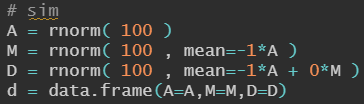
\includegraphics[scale=0.8]{fork1_code.png}
				\caption*{(c) R code}
			\end{figure}
			%
			\textcolor{blue}{Implications},
			%
			\begin{itemize}
				\item \ndsep{M}{D} \\
				\item \dsep{M}{D} \; | A
			\end{itemize}
			%
		\end{column}
		%
		\begin{column}{0.5\textwidth}  
			%
			\begin{equ}
				%
				M = \left\{ \begin{aligned} 
					A \leftarrow & \; f_{A}(U_{A}) \\
					M \leftarrow & \; f_{M}(A,U_{M}) \\
					D \leftarrow & \; f_{D}(A, U_{D}) \\
					U \sim & \; P(\pmb{U})
				\end{aligned} \right
				%
				\caption*{(a) structural model}
				%
			\end{equ}
			%
			\begin{figure}
				%
				\begin{tikzpicture}
					% nodes
					\node[formula] at (-2,0) {$U_{M}$};
					\node[formula] at (-1,-0.3) {$M$};
					\node[formula] at (1,1.5) {$U_{A}$};
					\node[formula] at (0,1) {$A$};
					\node[formula] at (2,0) {$U_{D}$};
					\node[formula] at (1,-0.3) {$D$};
					
					% paths
					\draw [{Circle [open]}-{latex}{Circle}](-1.7,0)--(-0.9,0); % Um->M
					%\draw [-{latex}](-0.9,0)--(0.9,0); % M->D
					\draw [{Circle [open]}-{latex}{Circle}](1.7,0)--(0.9,0); % Ud->D
					\draw [{Circle [color=red]}-{latex}](0.1,0.8)--(-0.9,0.1); % A->M
					\draw [-{latex}](0.1,0.75)--(0.9,0.1); % A->D
					\draw [{Circle [open]}-{latex}](0.9,1.3)--(0.1,0.8); % Ua->A
				\end{tikzpicture}
				%
				\caption*{(b) causal diagram}
				%
			\end{figure}
			%
		\end{column}
		%
	\end{columns}
	%
\end{frame}
%
%
\begin{lhframe}[rhgraphic={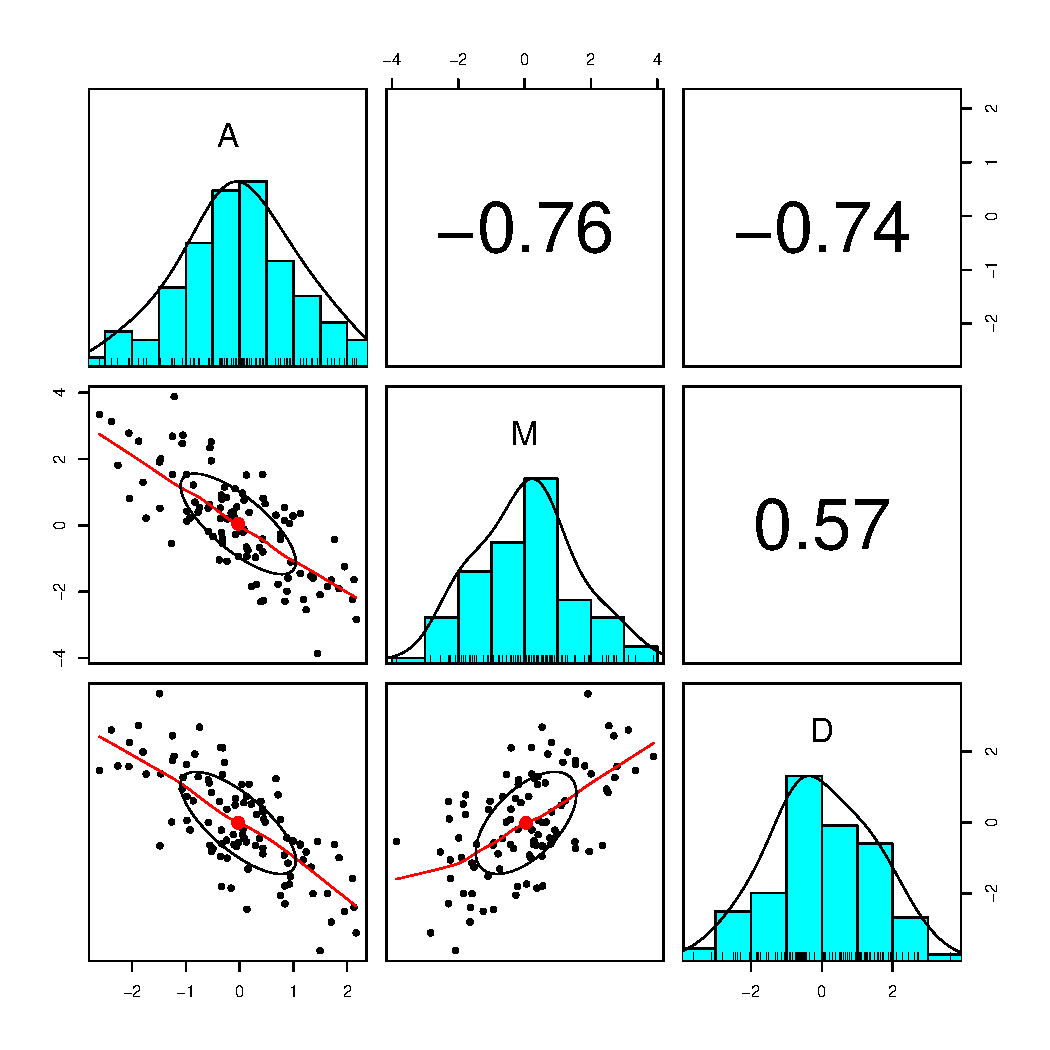
\includegraphics[scale=0.4]{fork1_panel.pdf}}]
	{``Eyeballing" analysis}
	
	based on \textcolor{blue}{correlation analysis},
	%
	\begin{itemize}
		%
		\item $cor(A, D)<0$ and $cor(M, D)>0$ goes in line of our ``rudimentary" understanding of the data.
		%
		\item why there is $cor(M, D)>0$? \\
		{\small (hint: univariate correlation)}
		%
		\item we \textcolor{blue}{include} $M$ as a covariate in our statistical model \\
		{\small (is our research hypothesis)}
		%
	\end{itemize}
	%
\end{lhframe}
%
%
\begin{lhframe}[rhgraphic={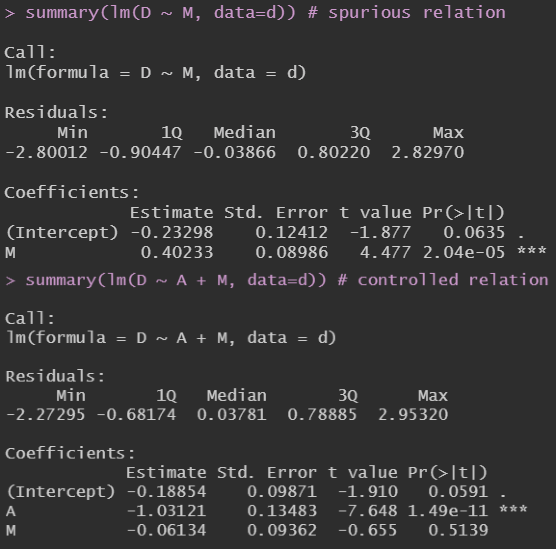
\includegraphics[scale=0.3]{fork1_reg.png}}]
	{Regression, regression!!}
	
	based on \textcolor{blue}{statistical analysis},
	%
	\begin{itemize}
		%
		\item we have two different stories, \\
		{\small (which one is the ``truth"?)}
		%
	\end{itemize}
	%
\end{lhframe}
%
%
\begin{lhframe}[rhgraphic={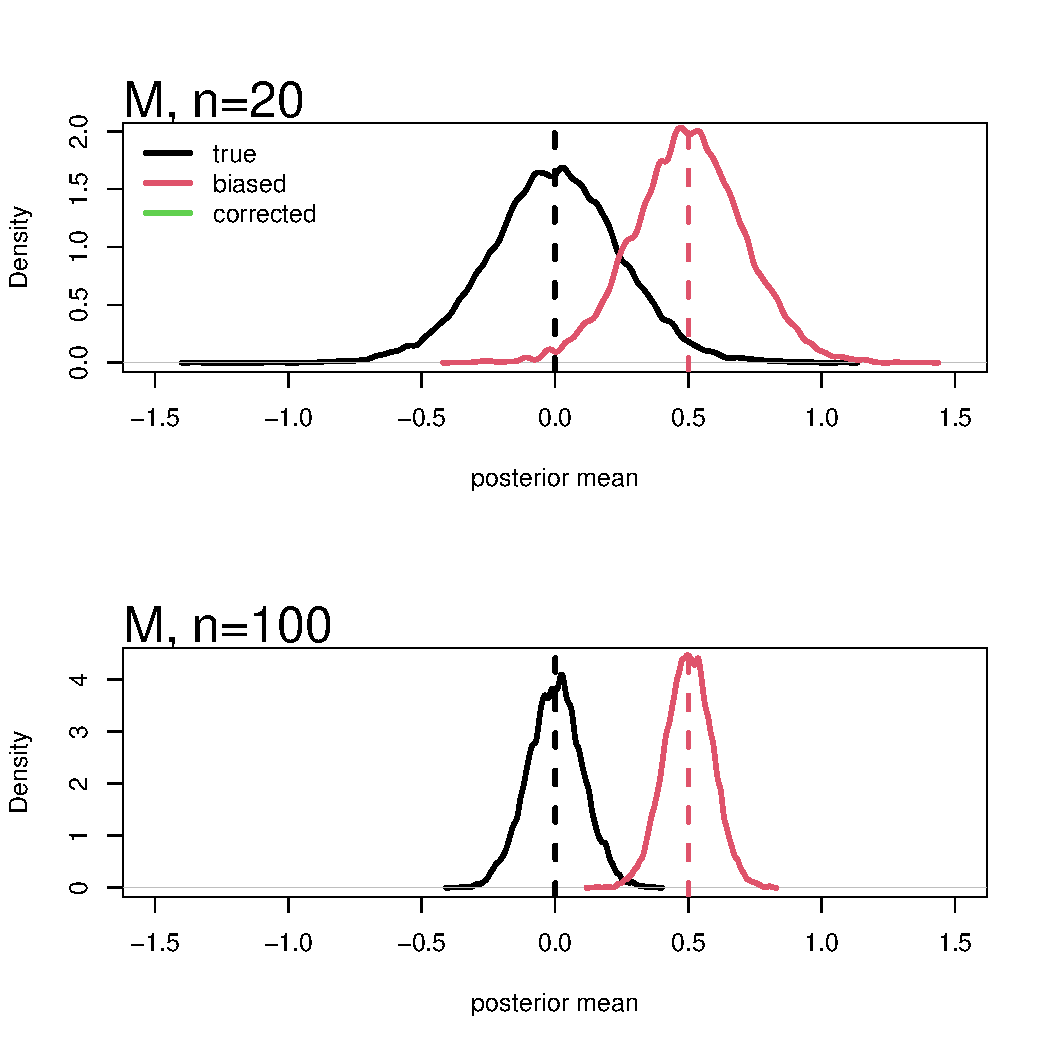
\includegraphics[scale=0.45]{fork1_samplesize.pdf}}]
	{I'll get more data!!}
	
	imagine we can continue sampling,
	%
	\begin{itemize}
		%
		\item top: $10,000$ samples $n=20$
		\item bottom: $10,000$ samples $n=100$
		%
	\end{itemize}

	under the \textcolor{blue}{incorrect model}, \\
	the larger the sample size,
	%
	\begin{itemize}
		%
		\item the more \textcolor{blue}{certain} you are about your \textcolor{blue}{biased} estimates \\
		{\small \alert{(the winner's curse)}}
		%
	\end{itemize}
	%
\end{lhframe}
%
%
\begin{frame}
	{The dream team!!}
	%
	\begin{columns}
		%
		\begin{column}{0.5\textwidth}
			%
			based on \textcolor{blue}{DAG} and \textcolor{blue}{statistical model},
			%
			\begin{itemize}
				%
				\item the 2nd D-separation rule requires you to control any noncollider to block the \textcolor{blue}{backdoor path}, \\
				i.e. \dsep{M}{D} \; | A \\
				%
				\item conditioning on $A$ we can find, \\
				{\small $E[D | do(m)] = E[\; E[D | M=m, A] \;]$} \\
				{\small (law of total expectation)}
				%
				\item then we can find the \\
				{\small $\text{ACE}(m) = E[D | do(m+1)] - E[D | do(m)]$ } \\
				{\small \textcolor{blue}{(Frisch-Waugh-Lovell theorem)} }
				%
			\end{itemize}
			%
		\end{column}
		%
		\begin{column}{0.5\textwidth}  
			%
			\begin{equ}
				%
				M = \left\{ \begin{aligned} 
					A \leftarrow & \; f_{A}(U_{A}) \\
					M \leftarrow & \; f_{M}(A,U_{M}) \\
					D \leftarrow & \; f_{D}(A, M, U_{D}) \\
					U \sim & \; P(\pmb{U})
				\end{aligned} \right
				%
				\caption*{(a) structural model}
				%
			\end{equ}
			%
			\begin{figure}
				%
				\begin{tikzpicture}
					% nodes
					\node[formula] at (-2,0) {$U_{M}$};
					\node[formula] at (-1,-0.3) {$M$};
					\node[formula] at (1,1.5) {$U_{A}$};
					\node[formula] at (0,1) {$A$};
					\node[formula] at (2,0) {$U_{D}$};
					\node[formula] at (1,-0.3) {$D$};
					
					% paths
					\draw [{Circle [open]}-{latex}{Circle}](-1.7,0)--(-0.9,0); % Um->M
					\draw [-{latex}](-0.9,0)--(0.9,0); % M->D
					\draw [{Circle [open]}-{latex}{Circle}](1.7,0)--(0.9,0); % Ud->D
					\draw [{Circle [color=red]}-{latex}](0.1,0.8)--(-0.9,0.1); % A->M
					\draw [-{latex}](0.1,0.75)--(0.9,0.1); % A->D
					\draw [{Circle [open]}-{latex}](0.9,1.3)--(0.1,0.8); % Ua->A
					
					% extra
					\node at (0,-0.25) {$(?)$}; % symbol
				\end{tikzpicture}
				%
				\caption*{(b) causal diagram}
				%
			\end{figure}
			%
		\end{column}
		%
	\end{columns}
	%
\end{frame}
%
%
\begin{lhframe}[rhgraphic={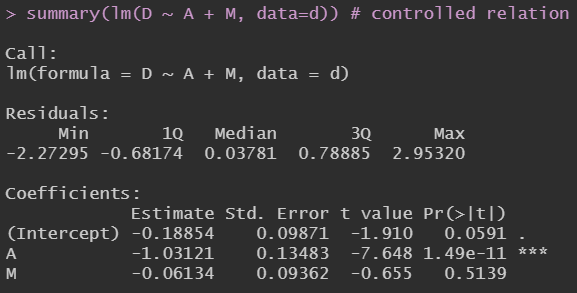
\includegraphics[scale=0.5]{fork1_reg2.png}}]
	{the dream team!!}
	
	based on \textcolor{blue}{DAG} and \textcolor{blue}{statistical analysis},
	%
	\begin{itemize}
		%
		\item the less biased model is the second, \\
		{\small \textcolor{blue}{(assuming our DAG is true)} }
		%
	\end{itemize}
	%
\end{lhframe}
%
%
\begin{frame}
	{So, what is going on?}
	
	\begin{figure*}
		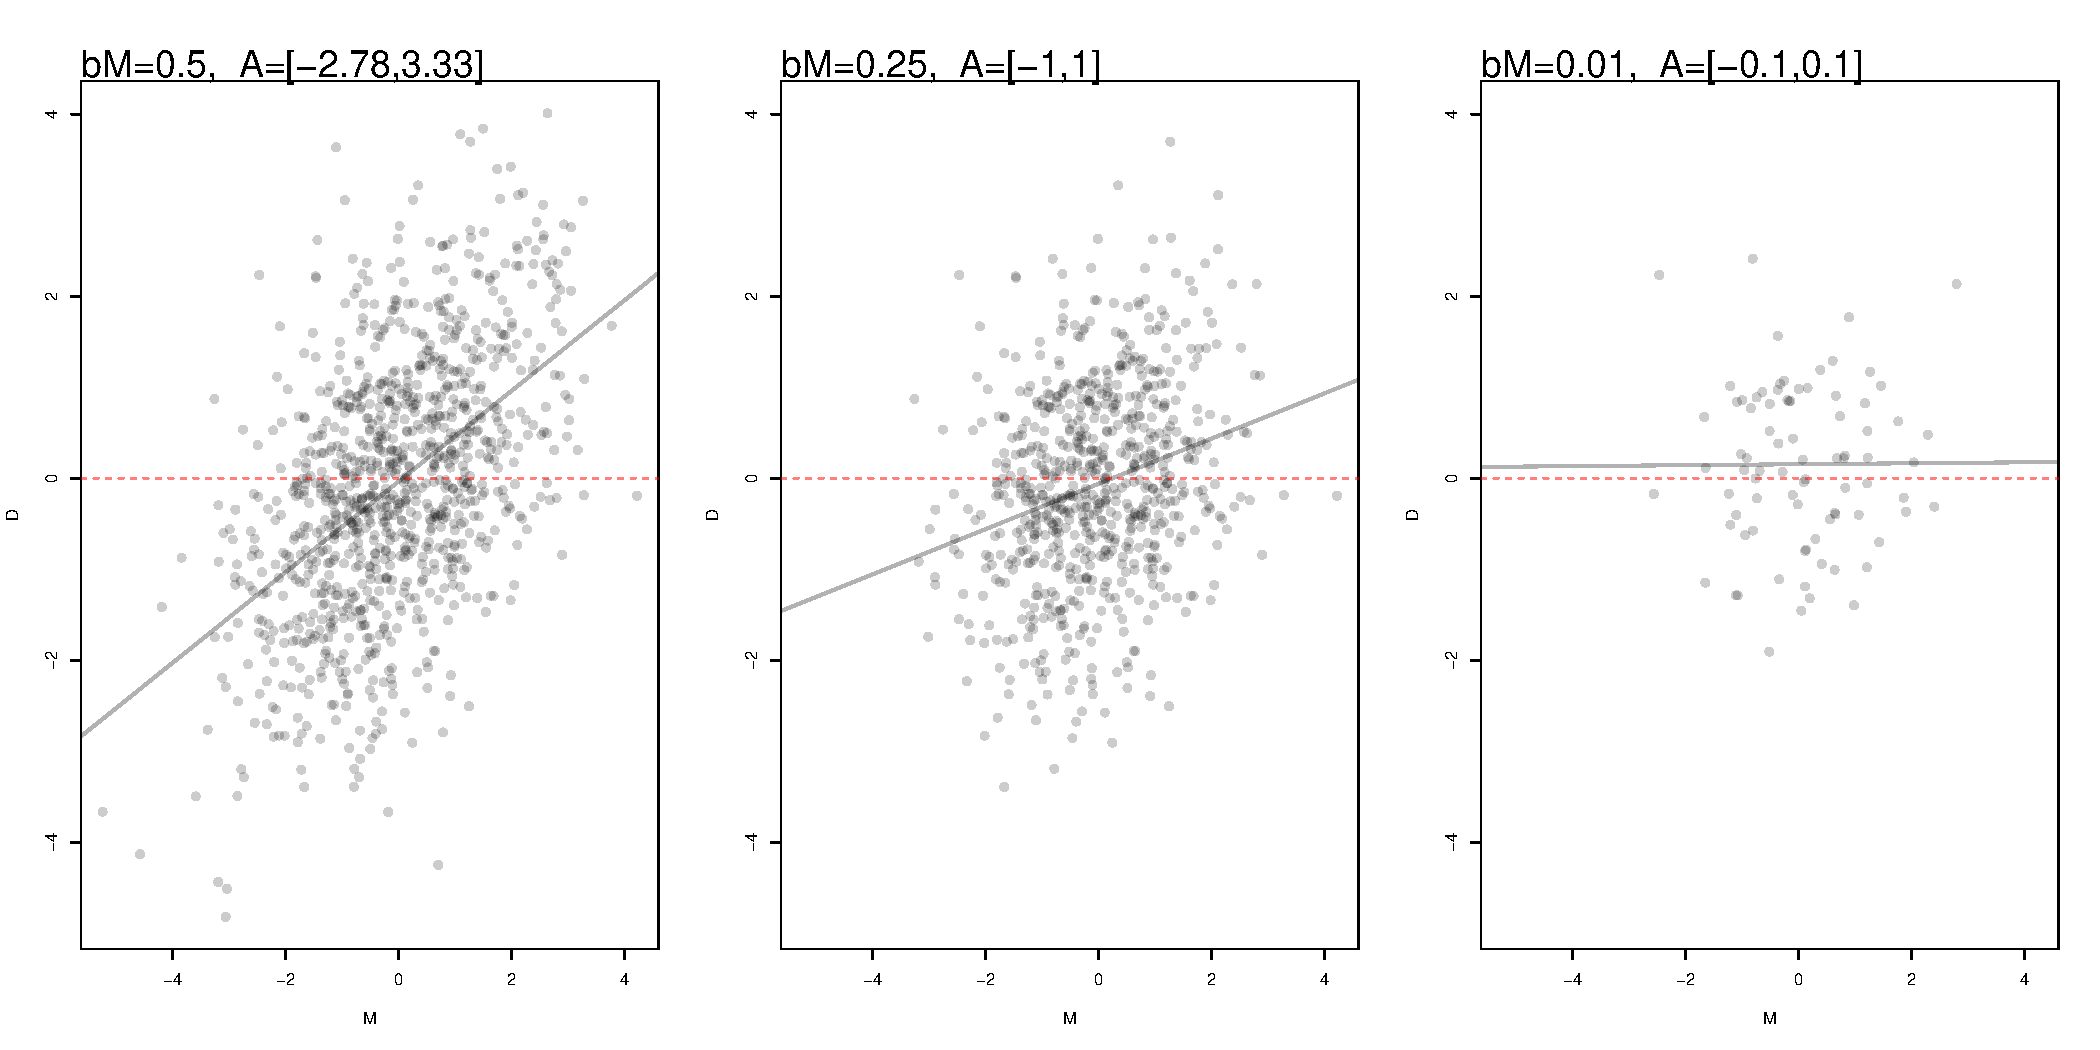
\includegraphics[width=\linewidth]{fork1_triptych.pdf}
	\end{figure*}
	%
\end{frame}
%
%
%%%%%%%%%%%%%%%%%%%%%%%%%%%%%%%%%%%%%%%%%%%%%%%%%%%%%%%%%%%
\subsection{Fork bias: masked relationships (a)}
%%%%%%%%%%%%%%%%%%%%%%%%%%%%%%%%%%%%%%%%%%%%%%%%%%%%%%%%%%%
%
%
\begin{frame}[t, negative]
	\subsectionpage
\end{frame}
%
%
\begin{frame}
	{Masked relationships (a)\footnote{\citet{McElreath_2020}, chapter 05 (p. 144)}}
	%
	\begin{columns}
		%
		\begin{column}{0.5\textwidth}
			%
			also known as,
			%
			\begin{itemize}
				%
				\item omitted variable bias
				\item an instance of \textcolor{blue}{fork bias}
				%
			\end{itemize}
			
			research question, 
			%
			\begin{itemize}
				%
				\item \textcolor{blue}{Does $N$ has a (direct) effect on $K$?}
				%
			\end{itemize}
			
			variables,
			%
			\begin{itemize}
				%
				\item M, mammal mass in kg.
				\item N, ratio neocortex over total brain mass
				\item K, Kcal. per gram of milk
				%
			\end{itemize}
			%
		\end{column}
		%
		\begin{column}{0.5\textwidth}  
			%
			\begin{equ}
				%
				M = \left\{ \begin{aligned} 
					M \leftarrow & \; f_{M}(U_{M}) \\
					N \leftarrow & \; f_{N}(M, U_{N}) \\
					K \leftarrow & \; f_{K}(M, N, U_{K}) \\
					U \sim & \; P(\pmb{U})
				\end{aligned} \right
				%
				\caption*{(a) structural model}
				%
			\end{equ}
			%
			\begin{figure}
				%
				\begin{tikzpicture}
					% nodes
					\node[formula] at (-2,0) {$U_{N}$};
					\node[formula] at (-1,-0.3) {$N$};
					\node[formula] at (1,1.5) {$U_{M}$};
					\node[formula] at (0,1) {$M$};
					\node[formula] at (2,0) {$U_{K}$};
					\node[formula] at (1,-0.3) {$K$};
					
					% paths
					\draw [{Circle [open]}-{latex}{Circle}](-1.7,0)--(-0.9,0); % Un->N
					\draw [-{latex}](-0.9,0)--(0.9,0); % N->K
					\draw [{Circle [open]}-{latex}{Circle}](1.7,0)--(0.9,0); % Uk->K
					\draw [{Circle [color=red]}-{latex}](0.1,0.8)--(-0.9,0.1); % M->N
					\draw [-{latex}](0.1,0.75)--(0.9,0.1); % M->K
					\draw [{Circle [open]}-{latex}](0.9,1.3)--(0.1,0.8); % Um->M
					
					% extra
					\node at (0,-0.25) {$(?)$}; % symbol
				\end{tikzpicture}
				%
				\caption*{(b) causal diagram}
				%
			\end{figure}
			%
		\end{column}
		%
	\end{columns}
	%
\end{frame}
%
%
\begin{frame}
	{Simulation setting}
	%
	\begin{columns}
		%
		\begin{column}{0.5\textwidth}
			%
			\begin{figure}
				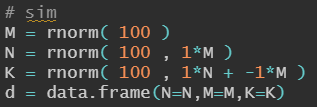
\includegraphics[scale=0.8]{fork2_code.png}
				\caption*{(c) R code}
			\end{figure}
			%
			\textcolor{blue}{Implications},
			%
			\begin{itemize}
				\item \ndsep{N}{K} \\
				\item \ndsep{N}{K} \; | M
			\end{itemize}
			%
		\end{column}
		%
		\begin{column}{0.5\textwidth}  
			%
			\begin{equ}
				%
				M = \left\{ \begin{aligned} 
					M \leftarrow & \; f_{M}(U_{M}) \\
					N \leftarrow & \; f_{N}(M,U_{N}) \\
					K \leftarrow & \; f_{K}(M, N, U_{K}) \\
					U \sim & \; P(\pmb{U})
				\end{aligned} \right
				%
				\caption*{(a) structural model}
				%
			\end{equ}
			%
			\begin{figure}
				%
				\begin{tikzpicture}
					% nodes
					\node[formula] at (-2,0) {$U_{N}$};
					\node[formula] at (-1,-0.3) {$N$};
					\node[formula] at (1,1.5) {$U_{M}$};
					\node[formula] at (0,1) {$M$};
					\node[formula] at (2,0) {$U_{K}$};
					\node[formula] at (1,-0.3) {$K$};
					
					% paths
					\draw [{Circle [open]}-{latex}{Circle}](-1.7,0)--(-0.9,0); % Un->N
					\draw [-{latex}](-0.9,0)--(0.9,0); % N->K
					\draw [{Circle [open]}-{latex}{Circle}](1.7,0)--(0.9,0); % Uk->K
					\draw [{Circle [color=red]}-{latex}](0.1,0.8)--(-0.9,0.1); % M->N
					\draw [-{latex}](0.1,0.75)--(0.9,0.1); % M->K
					\draw [{Circle [open]}-{latex}](0.9,1.3)--(0.1,0.8); % Um->M
				\end{tikzpicture}
				%
				\caption*{(b) causal diagram}
				%
			\end{figure}
			%
		\end{column}
		%
	\end{columns}
	%
\end{frame}
%
%
\begin{lhframe}[rhgraphic={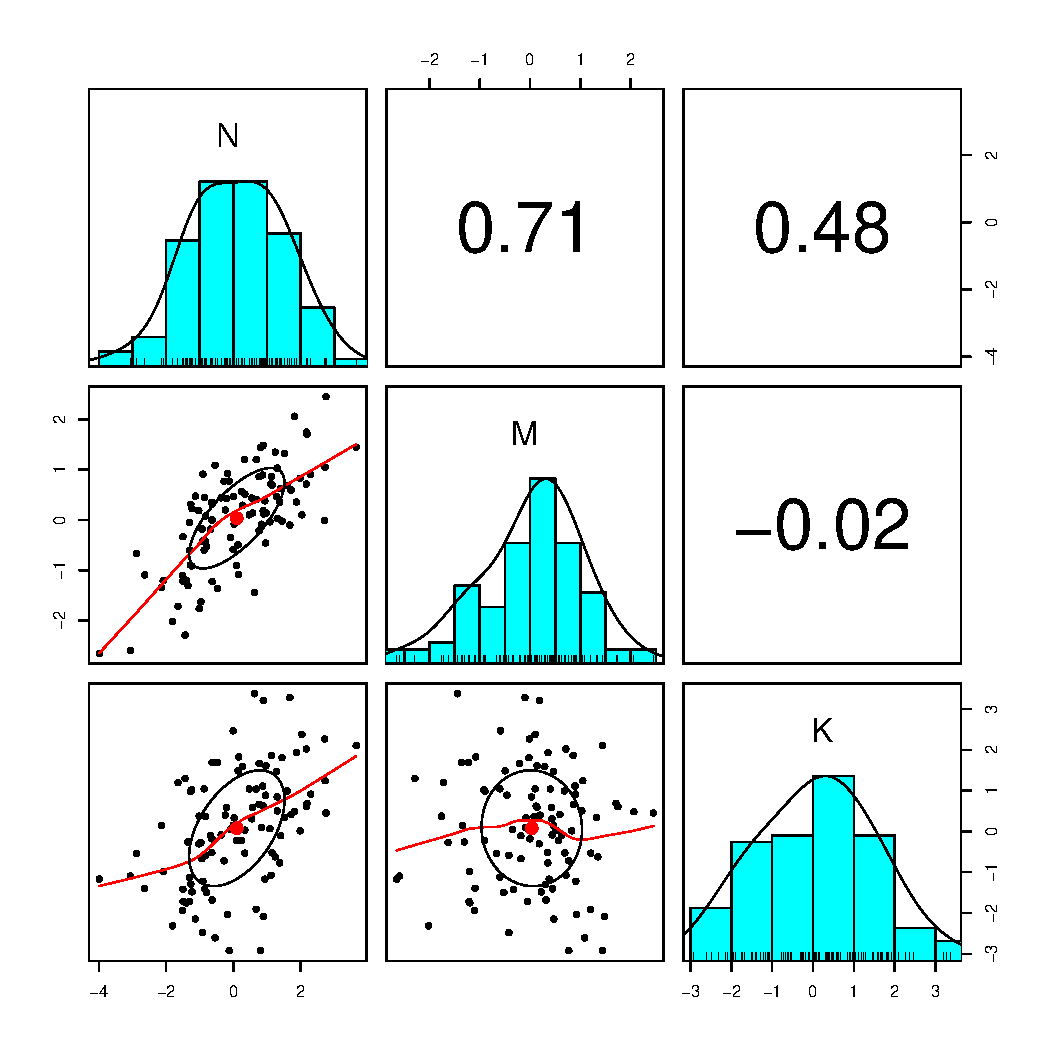
\includegraphics[scale=0.4]{fork2_panel.pdf}}]
	{``Eyeballing" analysis}
	
	based on \textcolor{blue}{correlation analysis},
	%
	\begin{itemize}
		%
		\item $cor(N, K)>0$ goes in line of our ``rudimentary" understanding of the data.
		%
		\item but why there is $cor(M, k) \approx 0$? \\
		{\small (hint: univariate correlation)}
		%
		\item we \textcolor{blue}{might not include} $M$ as a covariate in our statistical model
		%
	\end{itemize}
	%
\end{lhframe}
%
%
\begin{lhframe}[rhgraphic={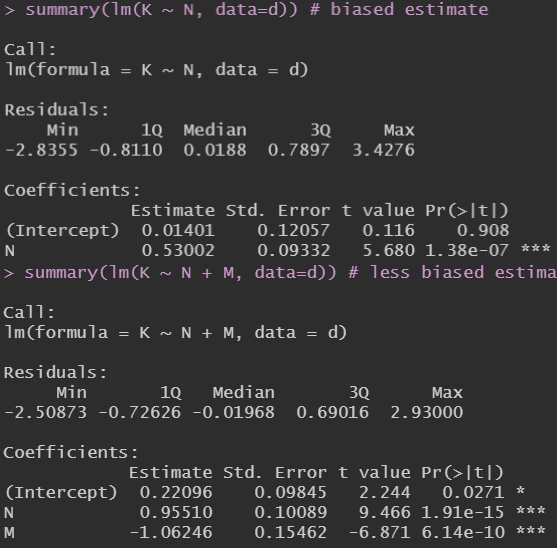
\includegraphics[scale=0.3]{fork2_reg.png}}]
	{Regression, regression!!}
	
	based on \textcolor{blue}{statistical analysis},
	%
	\begin{itemize}
		%
		\item we have two different stories, \\
		{\small (which one is the ``truth"?)}
		%
	\end{itemize}
	%
\end{lhframe}
%
%
\begin{lhframe}[rhgraphic={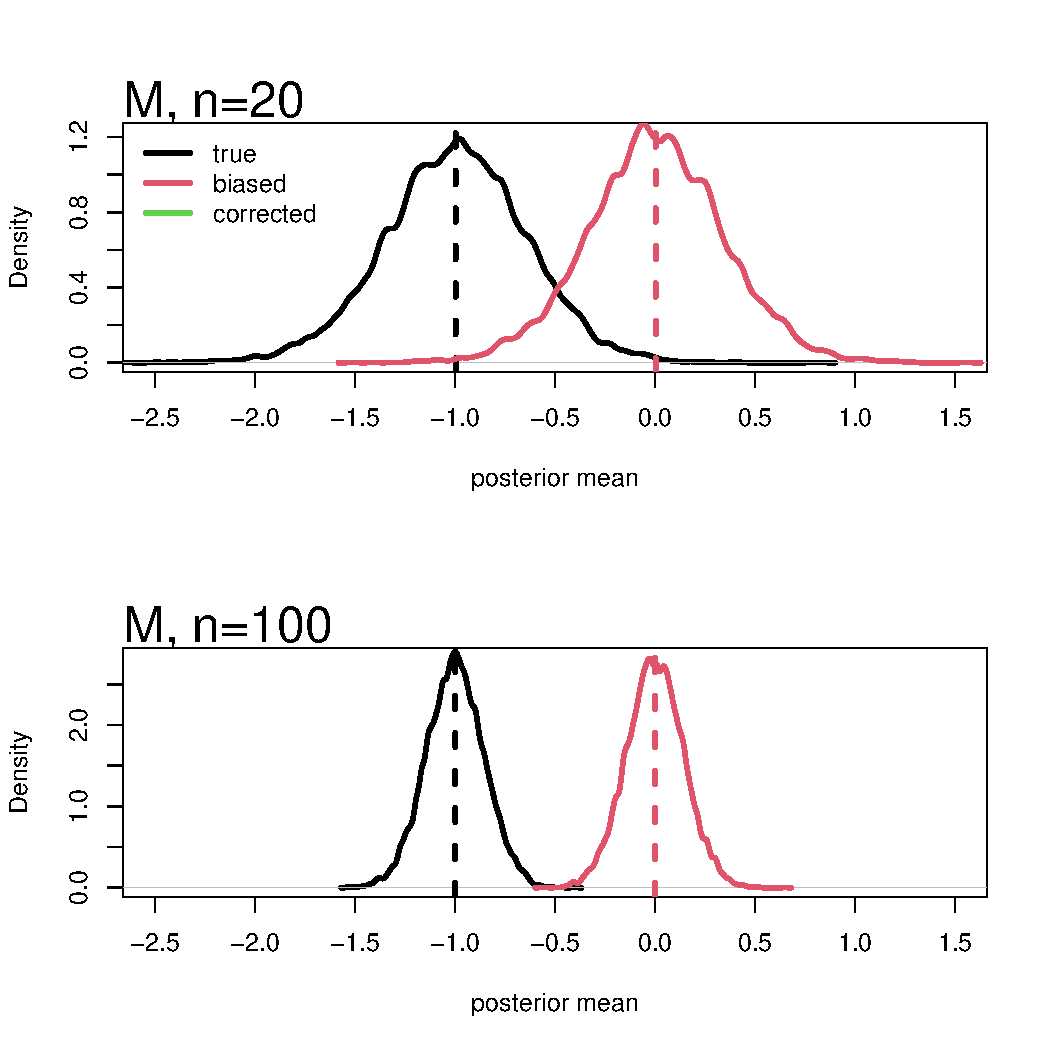
\includegraphics[scale=0.45]{fork2_samplesize.pdf}}]
	{I'll get more data!!}
	
	imagine we can continue sampling,
	%
	\begin{itemize}
		%
		\item top: $10,000$ samples $n=20$
		\item bottom: $10,000$ samples $n=100$
		%
	\end{itemize}
	
	under the \textcolor{blue}{incorrect model}, \\
	the larger the sample size,
	%
	\begin{itemize}
		%
		\item the more \textcolor{blue}{certain} you are about your \textcolor{blue}{biased} estimates
		%
	\end{itemize}
	%
\end{lhframe}
%
%
\begin{frame}
	{The dream team!!}
	%
	\begin{columns}
		%
		\begin{column}{0.5\textwidth}
			%
			based on \textcolor{blue}{DAG} and \textcolor{blue}{statistical model},
			%
			\begin{itemize}
				%
				\item the 2nd D-separation rule requires you to control any noncollider to block the \textcolor{blue}{backdoor path}, \\
				i.e. \ndsep{N}{K} \; | M \\
				%
				\item conditioning on $M$ we can find, \\
				{\small $E[K | do(n)] = E[\; E[K | N=n, M] \;]$} \\
				{\small (law of total expectation)}
				%
				\item then we can find the \\
				{\small $\text{ACE}(n) = E[D | do(n+1)] - E[D | do(n)]$ } \\
				{\small \textcolor{blue}{(Frisch-Waugh-Lovell theorem)} }
				%
			\end{itemize}
			%
		\end{column}
		%
		\begin{column}{0.5\textwidth}  
			%
			\begin{equ}
				%
				M = \left\{ \begin{aligned} 
					M \leftarrow & \; f_{M}(U_{M}) \\
					N \leftarrow & \; f_{N}(M,U_{N}) \\
					K \leftarrow & \; f_{K}(M, N, U_{K}) \\
					U \sim & \; P(\pmb{U})
				\end{aligned} \right
				%
				\caption*{(a) structural model}
				%
			\end{equ}
			%
			\begin{figure}
				%
				\begin{tikzpicture}
					% nodes
					\node[formula] at (-2,0) {$U_{N}$};
					\node[formula] at (-1,-0.3) {$N$};
					\node[formula] at (1,1.5) {$U_{M}$};
					\node[formula] at (0,1) {$M$};
					\node[formula] at (2,0) {$U_{K}$};
					\node[formula] at (1,-0.3) {$K$};
					
					% paths
					\draw [{Circle [open]}-{latex}{Circle}](-1.7,0)--(-0.9,0); % Un->N
					\draw [-{latex}](-0.9,0)--(0.9,0); % N->K
					\draw [{Circle [open]}-{latex}{Circle}](1.7,0)--(0.9,0); % Uk->K
					\draw [{Circle [color=red]}-{latex}](0.1,0.8)--(-0.9,0.1); % M->N
					\draw [-{latex}](0.1,0.75)--(0.9,0.1); % M->K
					\draw [{Circle [open]}-{latex}](0.9,1.3)--(0.1,0.8); % Um->M
					
					% extra
					\node at (0,-0.25) {$(?)$}; % symbol
				\end{tikzpicture}
				%
				\caption*{(b) causal diagram}
				%
			\end{figure}
			%
		\end{column}
		%
	\end{columns}
	%
\end{frame}
%
%
\begin{lhframe}[rhgraphic={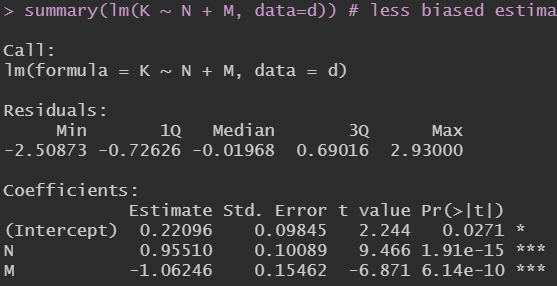
\includegraphics[scale=0.5]{fork2_reg2.png}}]
	{the dream team!!}
	
	based on \textcolor{blue}{DAG} and \textcolor{blue}{statistical analysis},
	%
	\begin{itemize}
		%
		\item the less biased model is the second, \\
		{\small \textcolor{blue}{(assuming our DAG is true)} }
		%
	\end{itemize}
	%
\end{lhframe}
%
%
\begin{frame}
	{So, what is going on?}
	
	\begin{figure*}
		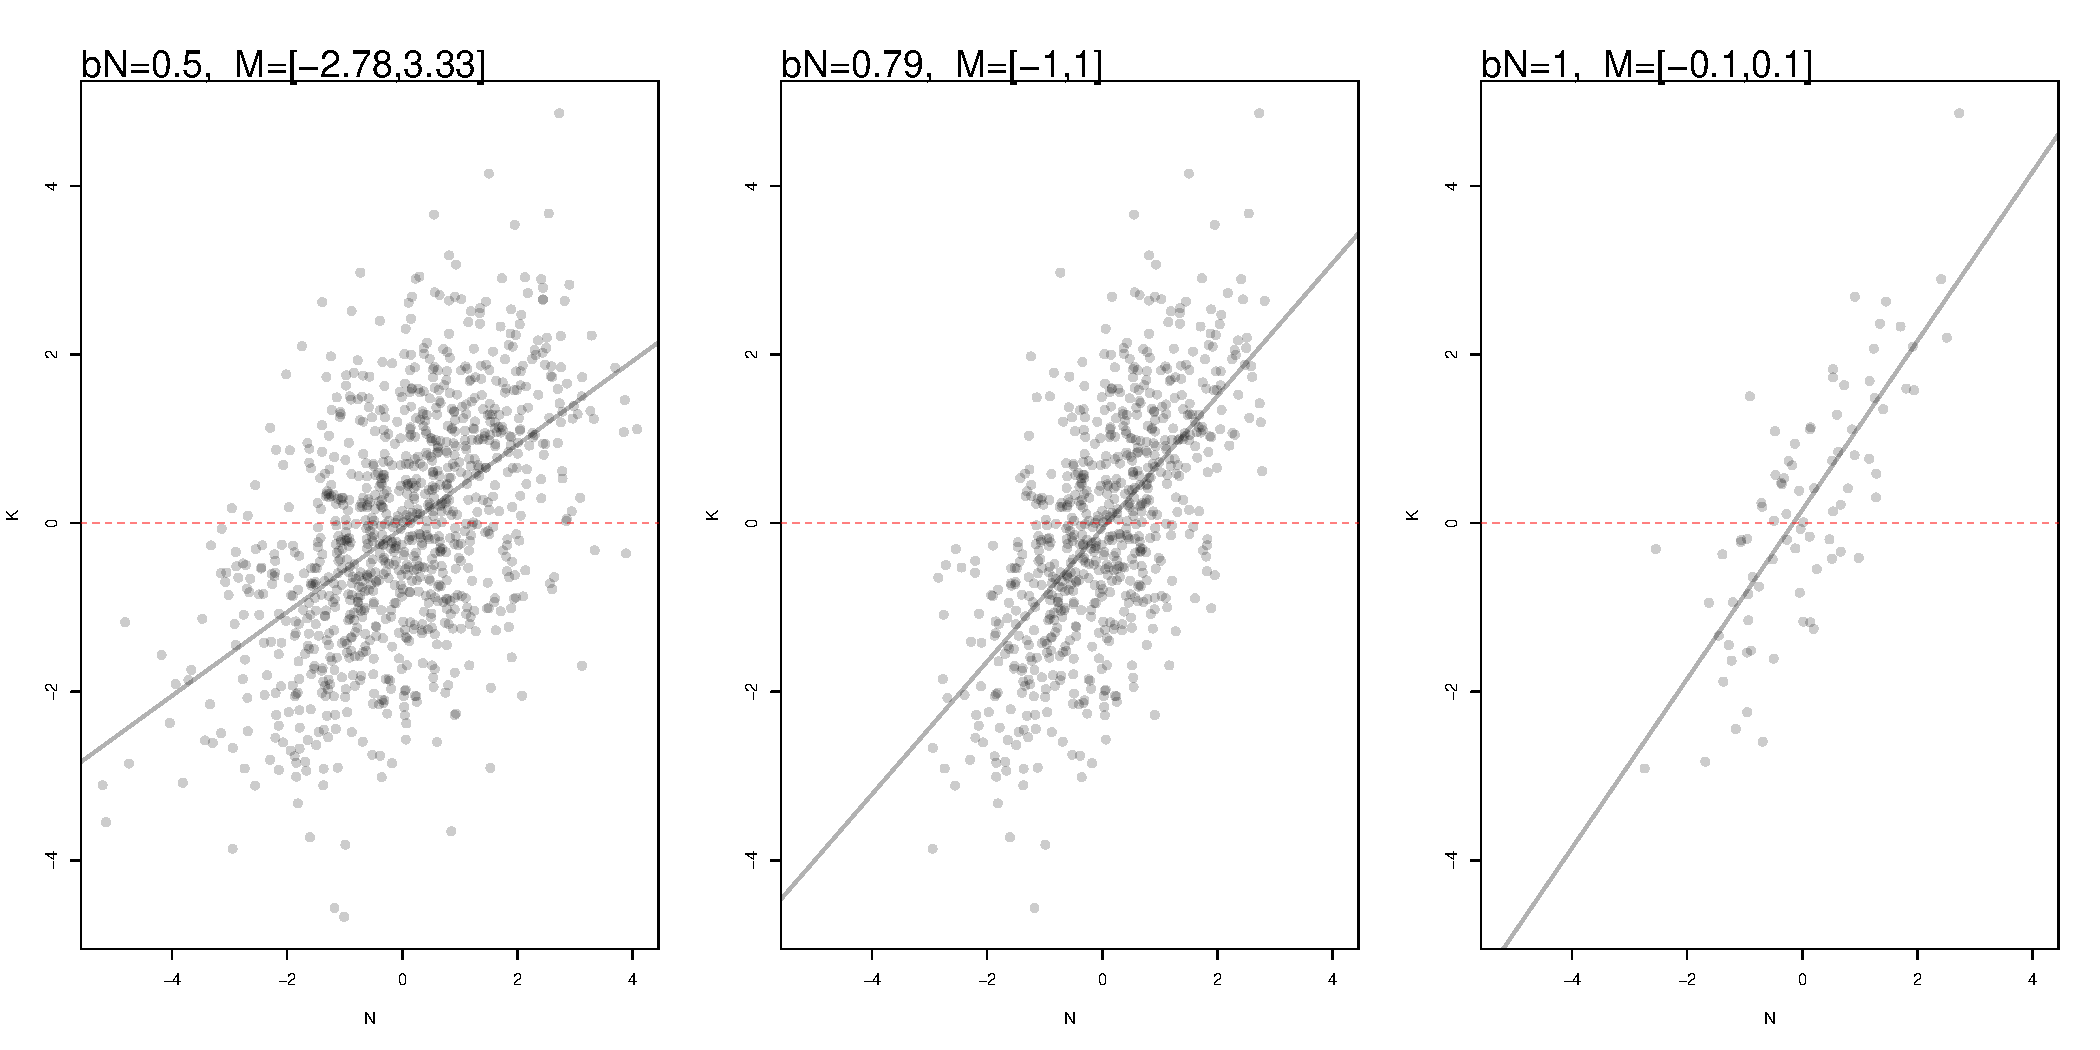
\includegraphics[width=\linewidth]{fork2_triptych.pdf}
	\end{figure*}
	%
\end{frame}
%
%
%%%%%%%%%%%%%%%%%%%%%%%%%%%%%%%%%%%%%%%%%%%%%%%%%%%%%%%%%%%
\subsection{Fork bias: masked relationships (b)}
%%%%%%%%%%%%%%%%%%%%%%%%%%%%%%%%%%%%%%%%%%%%%%%%%%%%%%%%%%%
%
%
\begin{frame}[t, negative]
	\subsectionpage
\end{frame}
%
%
\begin{frame}
	{Masked relationships (b)\footnote{\citet{McElreath_2020}, chapter 05 (p. 144)}}
	%
	\begin{columns}
		%
		\begin{column}{0.5\textwidth}
			%
			also known as,
			%
			\begin{itemize}
				%
				\item (unobserved) omitted variable bias
				\item an instance of \textcolor{blue}{fork bias}
				%
			\end{itemize}
			
			research question, 
			%
			\begin{itemize}
				%
				\item \textcolor{blue}{Does $N$ has a (direct) effect on $K$?}
				%
			\end{itemize}
			
			variables,
			%
			\begin{itemize}
				%
				\item $U_{X}$, unobservable (e.g. genetics)
				\item M, mammal mass in kg.
				\item N, neocortex over total brain mass
				\item K, Kcal. per gram of milk
				%
			\end{itemize}
			%
		\end{column}
		%
		\begin{column}{0.5\textwidth}  
			%
			\begin{equ}
				%
				M = \left\{ \begin{aligned} 
					N \leftarrow & \; f_{N}(U_{N},U_{X}) \\
					M \leftarrow & \; f_{M}(U_{M},U_{X}) \\
					K \leftarrow & \; f_{K}(M, N, U_{K}) \\
					U \sim & \; P(\pmb{U})
				\end{aligned} \right
				%
				\caption*{(a) structural model}
				%
			\end{equ}
			%
			\begin{figure}
				%
				\begin{tikzpicture}
					% nodes
					\node[formula] at (-1,1) {$U_{X}$};
					\node[formula] at (-2,0) {$U_{N}$};
					\node[formula] at (-1,-0.3) {$N$};
					\node[formula] at (1,1.5) {$U_{M}$};
					\node[formula] at (0,1) {$M$};
					\node[formula] at (2,0) {$U_{K}$};
					\node[formula] at (1,-0.3) {$K$};
					
					% paths
					\draw [{Circle [open]}-{latex}](-0.95,0.8)--(-0.95,0.05); % Ux->N
					\draw [-{latex}](-0.9,0.75)--(0,0.75); % Ux->M
					\draw [{Circle [open]}-{latex}{Circle}](-1.7,0)--(-0.9,0); % Un->N
					\draw [-{latex}](-0.9,0)--(0.9,0); % N->K
					\draw [{Circle [open]}-{latex}{Circle}](1.7,0)--(0.9,0); % Uk->K
					%\draw [-{latex}](-0.95,0.05)--(0,0.75); % N->M
					\draw [{Circle [color=red]}-{latex}](0,0.8)--(0.9,0.1); % M->K
					\draw [{Circle [open]}-{latex}](0.9,1.3)--(0.1,0.8); % Um->M
					
					% extra
					\node at (0,-0.25) {$(?)$}; % symbol
				\end{tikzpicture}
				%
				\caption*{(b) causal diagram}
				%
			\end{figure}
			%
		\end{column}
		%
	\end{columns}
	%
\end{frame}
%
%
\begin{frame}
	{Simulation setting}
	%
	\begin{columns}
		%
		\begin{column}{0.5\textwidth}
			%
			\begin{figure}
				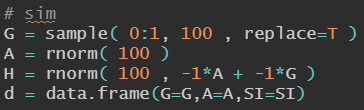
\includegraphics[scale=0.8]{fork3_code.png}
				\caption*{(c) R code}
			\end{figure}
			%
			\textcolor{blue}{Implications},
			%
			\begin{itemize}
				\item \ndsep{N}{K} \\
				\item \ndsep{N}{K} \; | M
			\end{itemize}
			%
		\end{column}
		%
		\begin{column}{0.5\textwidth}  
			%
			\begin{equ}
				%
				M = \left\{ \begin{aligned} 
					N \leftarrow & \; f_{N}(U_{N},U_{X}) \\
					M \leftarrow & \; f_{M}(U_{M},U_{X}) \\
					K \leftarrow & \; f_{K}(M, N, U_{K}) \\
					U \sim & \; P(\pmb{U})
				\end{aligned} \right
				%
				\caption*{(a) structural model}
				%
			\end{equ}
			%
			\begin{figure}
				%
				\begin{tikzpicture}
					% nodes
					\node[formula] at (-1,1) {$U_{X}$};
					\node[formula] at (-2,0) {$U_{N}$};
					\node[formula] at (-1,-0.3) {$N$};
					\node[formula] at (1,1.5) {$U_{M}$};
					\node[formula] at (0,1) {$M$};
					\node[formula] at (2,0) {$U_{K}$};
					\node[formula] at (1,-0.3) {$K$};
					
					% paths
					\draw [{Circle [open]}-{latex}](-0.95,0.8)--(-0.95,0.05); % Ux->N
					\draw [-{latex}](-0.9,0.75)--(0,0.75); % Ux->M
					\draw [{Circle [open]}-{latex}{Circle}](-1.7,0)--(-0.9,0); % Un->N
					\draw [-{latex}](-0.9,0)--(0.9,0); % N->K
					\draw [{Circle [open]}-{latex}{Circle}](1.7,0)--(0.9,0); % Uk->K
					%\draw [-{latex}](-0.95,0.05)--(0,0.75); % N->M
					\draw [{Circle [color=red]}-{latex}](0,0.8)--(0.9,0.1); % M->K
					\draw [{Circle [open]}-{latex}](0.9,1.3)--(0.1,0.8); % Um->M
				\end{tikzpicture}
				%
				\caption*{(b) causal diagram}
				%
			\end{figure}
			%
		\end{column}
		%
	\end{columns}
	%
\end{frame}
%
%
\begin{lhframe}[rhgraphic={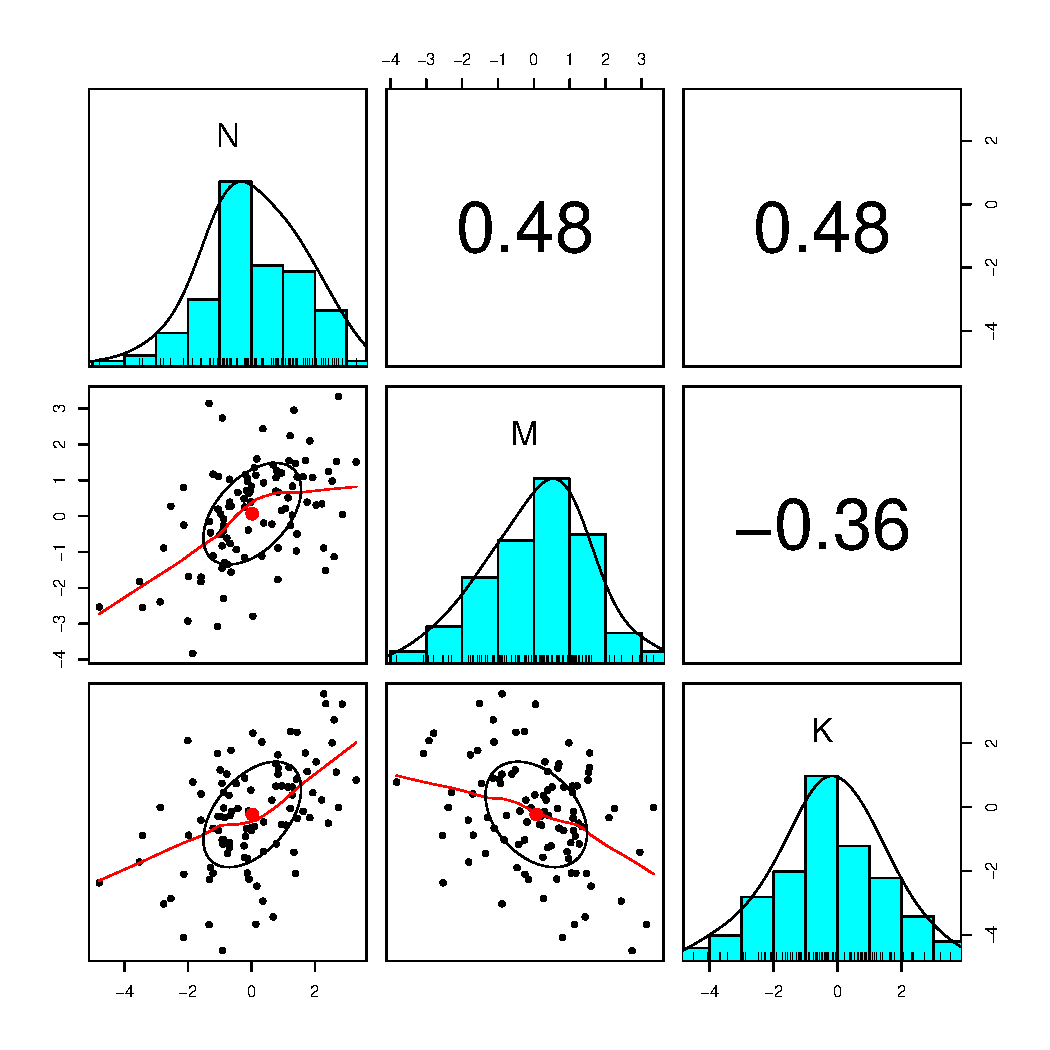
\includegraphics[scale=0.4]{fork3_panel.pdf}}]
	{``Eyeballing" analysis}
	
	based on \textcolor{blue}{correlation analysis},
	%
	\begin{itemize}
		%
		\item $cor(N, K)>0$ goes in line of our ``rudimentary" understanding of the data.
		%
		\item $cor(M, K)<0$ does NOT goes in line of our ``rudimentary" understanding of the data. \\
		{\small (hint: univariate correlation)}
		%
		\item we \textcolor{blue}{include} $M$ as a covariate in our statistical model \\
		{\small (by chance?)}
		%
	\end{itemize}
	%
\end{lhframe}
%
%
\begin{lhframe}[rhgraphic={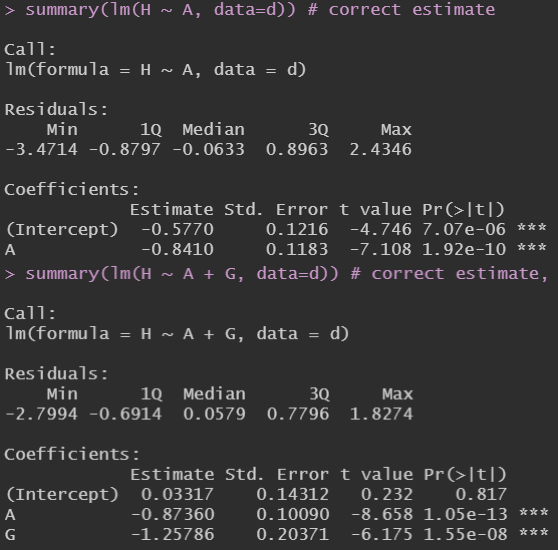
\includegraphics[scale=0.3]{fork3_reg.png}}]
	{Regression, regression!!}
	
	based on \textcolor{blue}{statistical analysis},
	%
	\begin{itemize}
		%
		\item we have two different stories, \\
		{\small (which one is the ``truth"?)}
		%
	\end{itemize}
	%
\end{lhframe}
%
%
\begin{lhframe}[rhgraphic={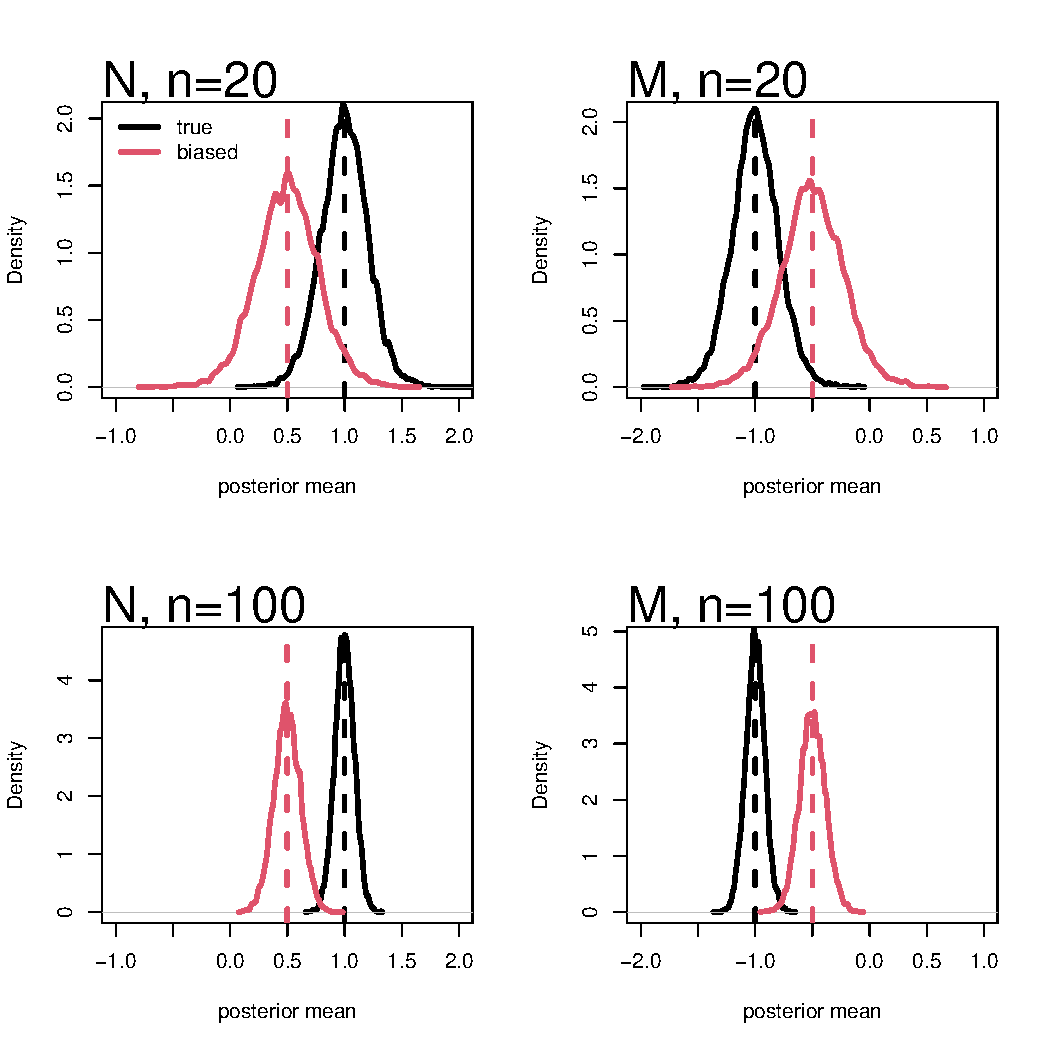
\includegraphics[scale=0.45]{fork3_samplesize.pdf}}]
	{I'll get more data!!}
	
	imagine we can continue sampling,
	%
	\begin{itemize}
		%
		\item top: $10,000$ samples $n=20$
		\item bottom: $10,000$ samples $n=100$
		%
	\end{itemize}
	
	under the \textcolor{blue}{incorrect model}, \\
	the larger the sample size,
	%
	\begin{itemize}
		%
		\item the more \textcolor{blue}{certain} you are about your \textcolor{blue}{biased} estimates
		%
	\end{itemize}
	%
\end{lhframe}
%
%
\begin{frame}
	{The dream team!!}
	%
	\begin{columns}
		%
		\begin{column}{0.5\textwidth}
			%
			based on \textcolor{blue}{DAG} and \textcolor{blue}{statistical model},
			%
			\begin{itemize}
				%
				\item the 2nd D-separation rule requires control on any noncollider to block the \textcolor{blue}{backdoor path}, \\
				i.e. \ndsep{N}{K} \; | $U_{X}$ \\
				{\small (but it is unobservable)}
				%
				\item still we use the 2nd D-separation rule by controlling for $M$, \\
				i.e. \ndsep{N}{K} \; | M \\
				%
				\item conditioning on $M$ we can still find, \\
				{\small $E[K | do(n)] = E[\; E[K | N=n, M] \;]$} \\
				{\small (law of total expectation)}
				%
				\item then we can find the \\
				{\small $\text{ACE}(n) = E[D | do(n+1)] - E[D | do(n)]$ } \\
				{\small \textcolor{blue}{(Frisch-Waugh-Lovell theorem??)} }
				%
			\end{itemize}
			%
		\end{column}
		%
		\begin{column}{0.5\textwidth}  
			%
			\begin{equ}
				%
				M = \left\{ \begin{aligned} 
					N \leftarrow & \; f_{N}(U_{N},U_{X}) \\
					M \leftarrow & \; f_{M}(U_{M},U_{X}) \\
					K \leftarrow & \; f_{K}(M, N, U_{K}) \\
					U \sim & \; P(\pmb{U})
				\end{aligned} \right
				%
				\caption*{(a) structural model}
				%
			\end{equ}
			%
			\begin{figure}
				%
				\begin{tikzpicture}
					% nodes
					\node[formula] at (-1,1) {$U_{X}$};
					\node[formula] at (-2,0) {$U_{N}$};
					\node[formula] at (-1,-0.3) {$N$};
					\node[formula] at (1,1.5) {$U_{M}$};
					\node[formula] at (0,1) {$M$};
					\node[formula] at (2,0) {$U_{K}$};
					\node[formula] at (1,-0.3) {$K$};
					
					% paths
					\draw [{Circle [open]}-{latex}](-0.95,0.8)--(-0.95,0.05); % Ux->N
					\draw [-{latex}](-0.9,0.75)--(0,0.75); % Ux->M
					\draw [{Circle [open]}-{latex}{Circle}](-1.7,0)--(-0.9,0); % Un->N
					\draw [-{latex}](-0.9,0)--(0.9,0); % N->K
					\draw [{Circle [open]}-{latex}{Circle}](1.7,0)--(0.9,0); % Uk->K
					%\draw [-{latex}](-0.95,0.05)--(0,0.75); % N->M
					\draw [{Circle [color=red]}-{latex}](0,0.8)--(0.9,0.1); % M->K
					\draw [{Circle [open]}-{latex}](0.9,1.3)--(0.1,0.8); % Um->M
					
					% extra
					\node at (0,-0.25) {$(?)$}; % symbol
				\end{tikzpicture}
				%
				\caption*{(b) causal diagram}
				%
			\end{figure}
			%
		\end{column}
		%
	\end{columns}
	%
\end{frame}
%
%
\begin{lhframe}[rhgraphic={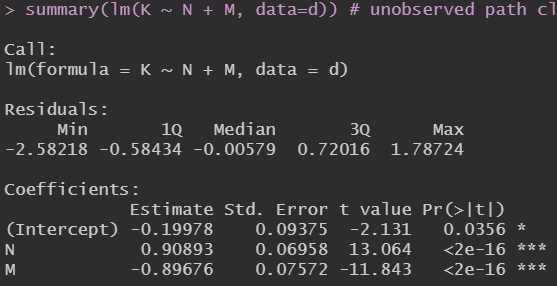
\includegraphics[scale=0.5]{fork3_reg2.png}}]
	{the dream team!!}
	
	based on \textcolor{blue}{DAG} and \textcolor{blue}{statistical analysis},
	%
	\begin{itemize}
		%
		\item the less biased model is the second, \\
		{\small \textcolor{blue}{(assuming our DAG is true)} }
		%
	\end{itemize}
	%
\end{lhframe}
%
%
\begin{frame}
	{So, what is going on?}
	
	\begin{figure*}
		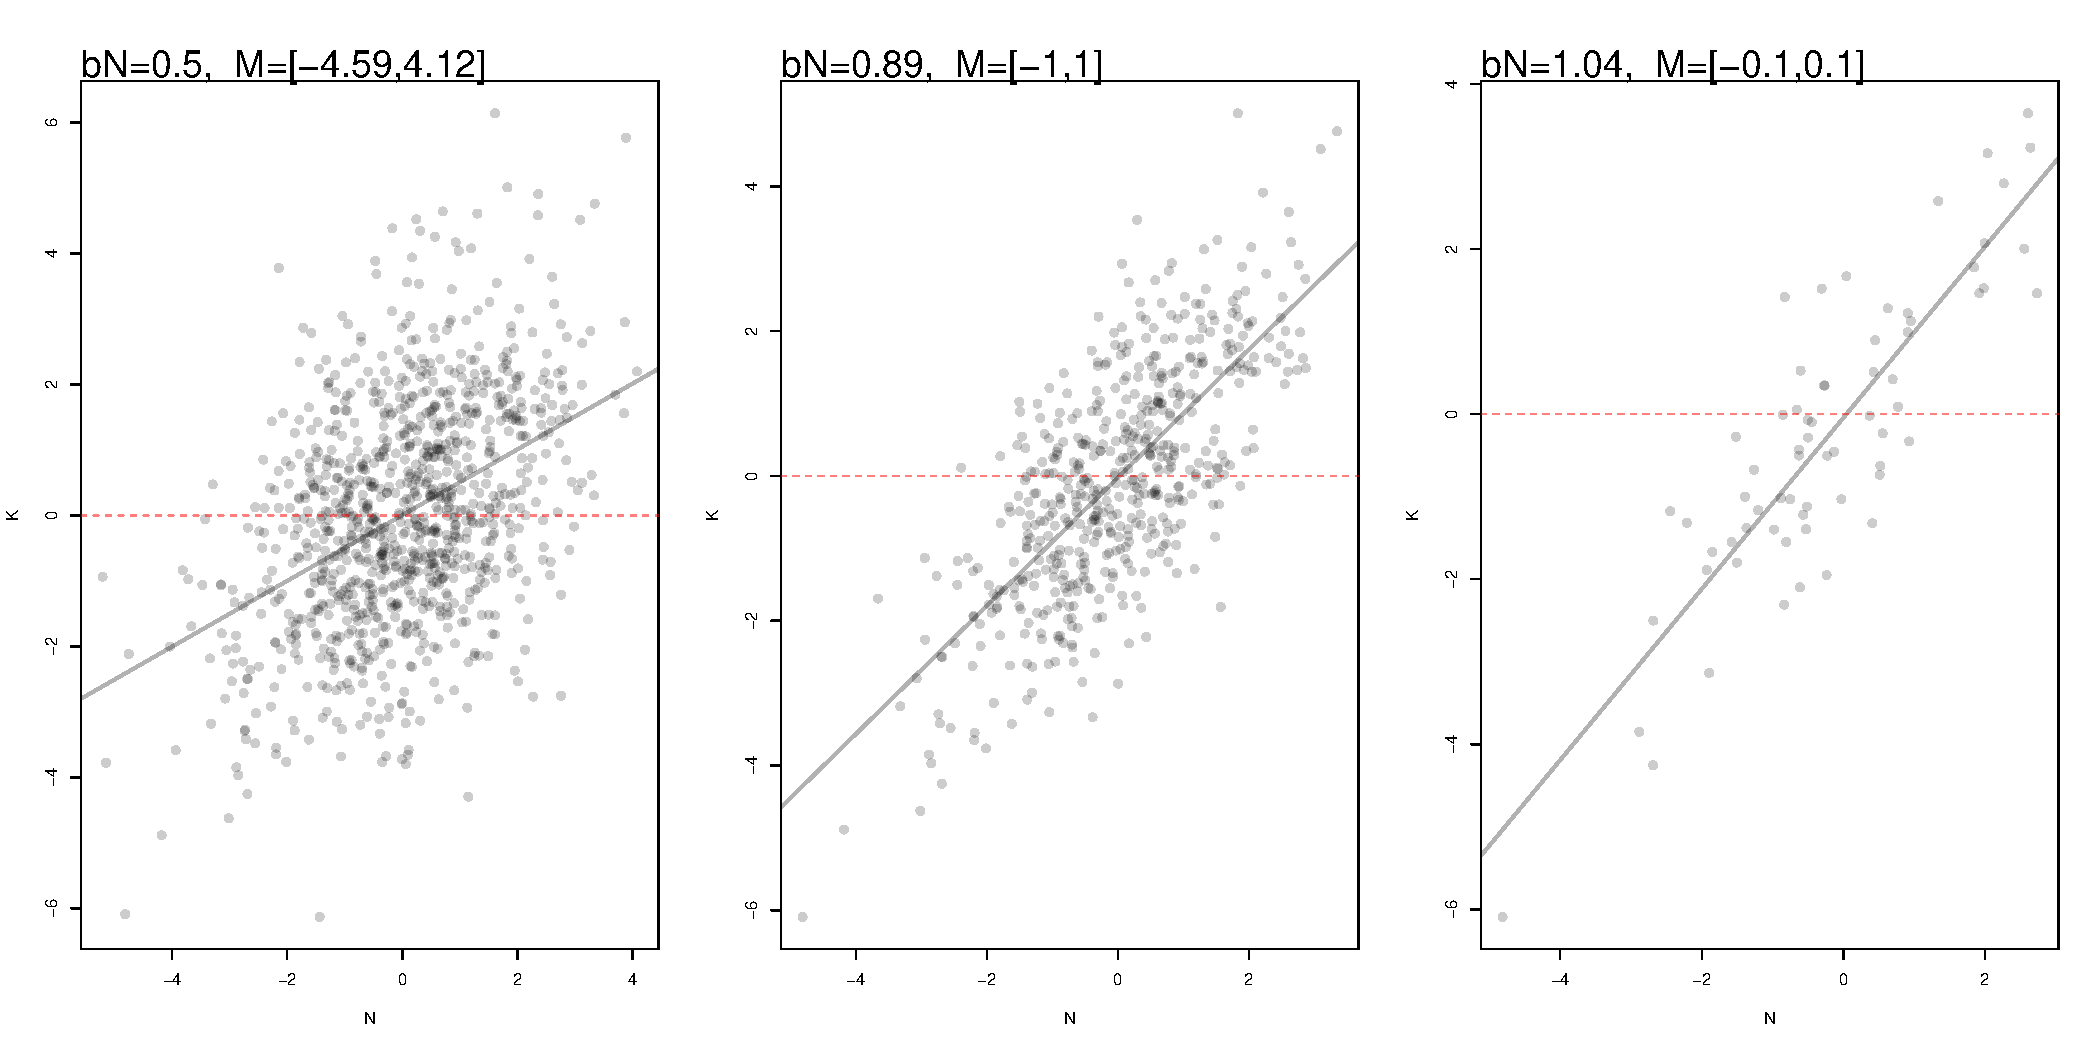
\includegraphics[width=\linewidth]{fork3_triptych.pdf}
	\end{figure*}
	%
\end{frame}
%
%
\begin{frame}
	{Similar scenario, unobserved masked\footnote{\citet{Cinelli_et_al_2021} (p. 3), \citet{McElreath_2022}, lecture 6}}
	%
	\begin{columns}
		%
		\begin{column}{0.5\textwidth}
			%
			research question, 
			%
			\begin{itemize}
				%
				\item \textcolor{blue}{Does $E$ has a (direct) effect on $I$?}
				%
			\end{itemize}
			
			variables,
			%
			\begin{itemize}
				%
				\item $U_{X}$, unobservable \\
				(e.g. family context)
				\item V, personal values
				\item E, education
				\item I, income
				%
			\end{itemize}
			%
			
			then,
			%
			\begin{itemize}
				%
				\item we need to control by $V$ to get an unbiased estimate of $E \rightarrow I$
				%
			\end{itemize}
			%
		\end{column}
		%
		\begin{column}{0.5\textwidth}  
			%
			\begin{equ}
				%
				M = \left\{ \begin{aligned} 
					V \leftarrow & \; f_{M}(U_{V},U_{X}) \\
					E \leftarrow & \; f_{E}(V,U_{E}) \\
					I \leftarrow & \; f_{I}(E, U_{X}, U_{I}) \\
					U \sim & \; P(\pmb{U})
				\end{aligned} \right
				%
				\caption*{(a) structural model}
				%
			\end{equ}
			%
			\begin{figure}
				%
				\begin{tikzpicture}
					% nodes
					\node[formula] at (-2,0.8) {$U_{V}$};
					\node[formula] at (-1,1) {$V$};
					\node[formula] at (-2,0) {$U_{E}$};
					\node[formula] at (-1,-0.3) {$E$};
					\node[formula] at (-0.1,1.05) {$U_{X}$};
					\node[formula] at (2,0) {$U_{I}$};
					\node[formula] at (1,-0.3) {$I$};
					
					% paths
					\draw [{Circle [open]}-{latex}](-1.7,0.75)--(-1,0.75); % Uv->V
					\draw [{Circle[color=red]}-{latex}](-0.95,0.8)--(-0.95,0.05); % V->E
					\draw [-{latex}](0,0.75)--(-0.9,0.75); % Ux->V
					\draw [{Circle [open]}-{latex}{Circle}](-1.7,0)--(-0.9,0); % Ue->E
					\draw [-{latex}](-0.9,0)--(0.9,0); % E->I
					\draw [{Circle [open]}-{latex}{Circle}](1.7,0)--(0.9,0); % Ui->I
					\draw [{Circle [open]}-{latex}](0,0.8)--(0.9,0.1); % Ux->I
					
					% extra
					\node at (0,-0.25) {$(?)$}; % symbol
				\end{tikzpicture}
				%
				\caption*{(b) causal diagram}
				%
			\end{figure}
			%
		\end{column}
		%
	\end{columns}
	%
\end{frame}
%
%
%%%%%%%%%%%%%%%%%%%%%%%%%%%%%%%%%%%%%%%%%%%%%%%%%%%%%%%%%%%
\subsection{Fork bias: multicollinearity}
%%%%%%%%%%%%%%%%%%%%%%%%%%%%%%%%%%%%%%%%%%%%%%%%%%%%%%%%%%%
%
%
\begin{frame}[t, negative]
	\subsectionpage
\end{frame}
%
%
\begin{frame}
	{Multicollinearity\footnote{\citet{McElreath_2020}, chapter 06 (p. 163)}}
	%
	\begin{columns}
		%
		\begin{column}{0.5\textwidth}
			%
			also known as,
			%
			\begin{itemize}
				%
				\item \textcolor{blue}{extreme case} of masked relationships
				\item an instance of \textcolor{blue}{fork bias}
				%
			\end{itemize}
			
			research question, 
			%
			\begin{itemize}
				%
				\item \textcolor{blue}{Should we include $RL$ in our model?}
				%
			\end{itemize}
			
			variables,
			%
			\begin{itemize}
				%
				\item $U_{X}$, unobservable \\
				(e.g. genetics and context)
				\item LL, individual's left leg
				\item RL, individual's right leg
				\item H, individual's height
				%
			\end{itemize}
			%
		\end{column}
		%
		\begin{column}{0.5\textwidth}  
			%
			\begin{equ}
				%
				M = \left\{ \begin{aligned} 
					LL \leftarrow & \; f_{L}(U_{X}) \\
					RL \leftarrow & \; f_{L}(U_{X}) \\
					H \leftarrow & \; f_{K}(RL,LL) \\
					U \sim & \; P(\pmb{U})
				\end{aligned} \right
				%
				\caption*{(a) structural model}
				%
			\end{equ}
			%
			\begin{figure}
				%
				\begin{tikzpicture}
					% nodes
					\node[formula] at (-1,1) {$U_{X}$};
					\node[formula] at (-1,-0.3) {$LL$};
					\node[formula] at (0,1) {$RL$};
					%\node[formula] at (2,0) {$U_{H}$};
					\node[formula] at (1,-0.3) {$H$};
					
					% paths
					\draw [{Circle [open]}-{latex}](-0.95,0.8)--(-0.95,0.05); % Ux->LL
					\draw [-{latex}](-0.9,0.75)--(0,0.75); % Ux->RL
					\draw [{Circle}-{latex}{Circle}](-1,0)--(1,0); % LL->H
					%\draw [{Circle[open]}-{latex}{Circle}](1.7,0)--(0.9,0); % Uh->H
					\draw [{Circle[color=red]}-{latex}](0,0.8)--(0.9,0.05); % RL->H
					
					% extra
					\node at (0,-0.25) {$(?)$}; % symbol
				\end{tikzpicture}
				%
				\caption*{(b) causal diagram}
				%
			\end{figure}
			%
		\end{column}
		%
	\end{columns}
	%
\end{frame}
%
%
\begin{frame}
	{Simulation setting}
	%
	\begin{columns}
		%
		\begin{column}{0.5\textwidth}
			%
			\begin{figure}
				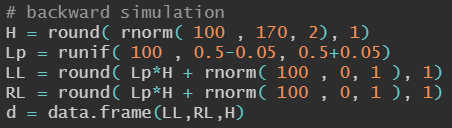
\includegraphics[scale=0.7]{fork4_code.png}
				\caption*{(c) R code}
			\end{figure}
			%
			\textcolor{blue}{Implications},
			%
			\begin{itemize}
				\item \ndsep{LL}{RL} \\
			\end{itemize}
			%
		\end{column}
		%
		\begin{column}{0.5\textwidth}  
			%
			\begin{equ}
				%
				M = \left\{ \begin{aligned} 
					LL \leftarrow & \; f_{L}(U_{X}) \\
					RL \leftarrow & \; f_{L}(U_{X}) \\
					H \leftarrow & \; f_{K}(RL,LL) \\
					U \sim & \; P(\pmb{U})
				\end{aligned} \right
				%
				\caption*{(a) structural model}
				%
			\end{equ}
			%
			\begin{figure}
				%
				\begin{tikzpicture}
					% nodes
					\node[formula] at (-1,1) {$U_{X}$};
					\node[formula] at (-1,-0.3) {$LL$};
					\node[formula] at (0,1) {$RL$};
					%\node[formula] at (2,0) {$U_{H}$};
					\node[formula] at (1,-0.3) {$H$};
					
					% paths
					\draw [{Circle [open]}-{latex}](-0.95,0.8)--(-0.95,0.05); % Ux->LL
					\draw [-{latex}](-0.9,0.75)--(0,0.75); % Ux->RL
					\draw [{Circle}-{latex}{Circle}](-1,0)--(1,0); % LL->H
					%\draw [{Circle[open]}-{latex}{Circle}](1.7,0)--(0.9,0); % Uh->H
					\draw [{Circle[color=red]}-{latex}](0,0.8)--(0.9,0.05); % RL->H
				\end{tikzpicture}
				%
				\caption*{(b) causal diagram}
				%
			\end{figure}
			%
		\end{column}
		%
	\end{columns}
	%
\end{frame}
%
%
\begin{lhframe}[rhgraphic={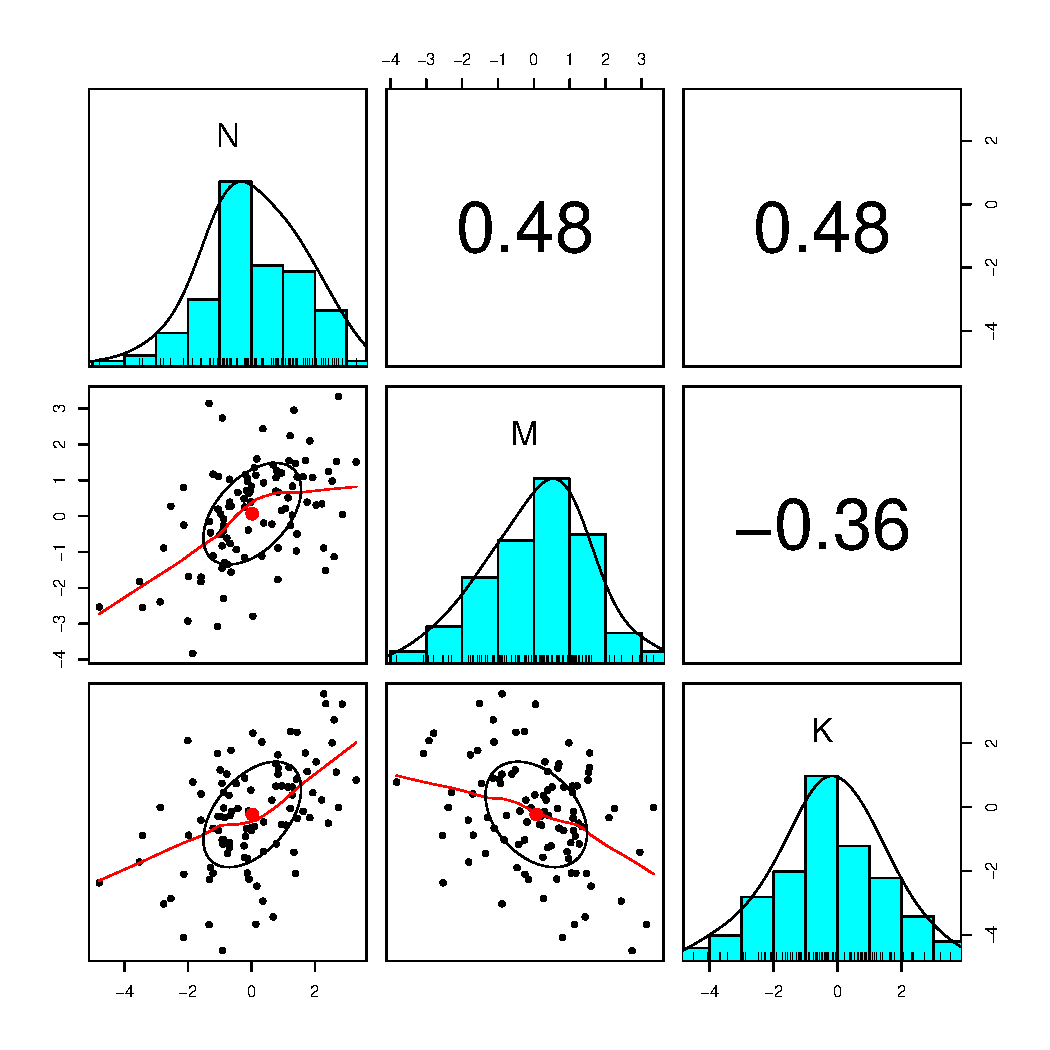
\includegraphics[scale=0.4]{fork4_panel.pdf}}]
	{``Eyeballing" analysis}
	
	based on \textcolor{blue}{correlation analysis},
	%
	\begin{itemize}
		%
		\item $cor(LL, H)>0$, $cor(RL, H)>0$ and $cor(LL, RL)>0$ goes in line of our ``understanding" of the data.
		%
		\item we \textcolor{blue}{might not include} $RL$ as a covariate in our statistical model \\
		{\small (based on \textcolor{blue}{univariate} correlation)} 
		%
	\end{itemize}
	%
\end{lhframe}
%
%
\begin{lhframe}[rhgraphic={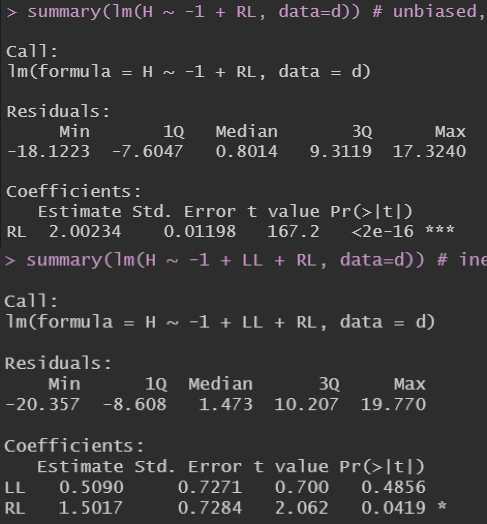
\includegraphics[scale=0.35]{fork4_reg.png}}]
	{Regression, regression!!}
	
	based on \textcolor{blue}{statistical analysis},
	%
	\begin{itemize}
		%
		\item the second regression show a smaller effect of LL,
		\item the second regression show way larger SE values \\
		{\small (not rejecting the null)}
		%
	\end{itemize}
	%
\end{lhframe}
%
%
\begin{lhframe}[rhgraphic={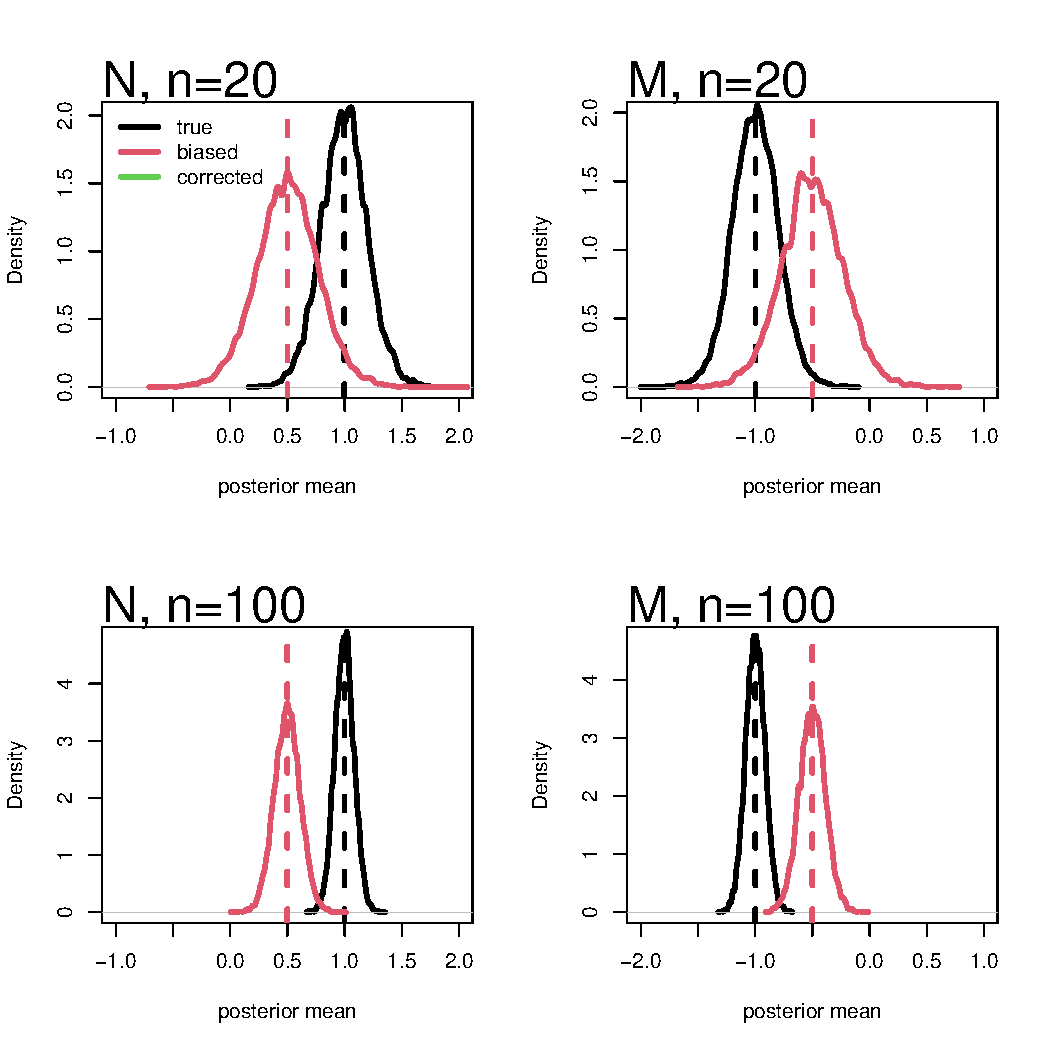
\includegraphics[scale=0.39]{fork4_samplesize.pdf}}]
	{I'm sure data won't help}
	
	imagine we can continue sampling,
	%
	\begin{itemize}
		%
		\item top: $10,000$ samples $n=20$
		\item bottom: $10,000$ samples $n=100$
		%
	\end{itemize}
	
	under the \textcolor{blue}{incorrect model}, \\
	the larger the sample size,
	%
	\begin{itemize}
		%
		\item the less \textcolor{blue}{certain} are your \textcolor{blue}{biased} estimates
		%
	\end{itemize}
	%
\end{lhframe}
%
%
\begin{frame}
	{Not so great now??}
	%
	\begin{columns}
		%
		\begin{column}{0.5\textwidth}
			%
			based on \textcolor{blue}{DAG} and \textcolor{blue}{statistical model},
			%
			\begin{itemize}
				%
				\item the 2nd D-separation rule requires control on any noncollider to block the \textcolor{blue}{backdoor path}, \\
				i.e. \ndsep{LL}{H} \; | $U_{X}$ \\
				{\small (but it is unobservable)}
				%
				\item we still use the 2nd D-separation rule by controlling for $RL$, but still we have \ndsep{LL}{H} \; | RL \\
				%
				\item \textcolor{blue}{issue goes beyond the backdoor path} \\
				the issue is that $RL$ and $LL$ give the same information to the model, \\
				i.e. they form a singular matrix, \\
				{\small (is like having a causal model like b) }
				%
			\end{itemize}
			%
		\end{column}
		%
		\begin{column}{0.5\textwidth}  
			%
			\begin{equ}
				%
				M = \left\{ \begin{aligned} 
					LL = & \; RL \\
					RL \leftarrow & \; f_{L}(U_{X}) \\
					H \leftarrow & \; f_{K}(RL) \\
					U \sim & \; P(\pmb{U})
				\end{aligned} \right
				%
				\caption*{(a) structural model}
				%
			\end{equ}
			%
			\begin{figure}
				%
				\begin{tikzpicture}
					% nodes
					\node[formula] at (-1,1) {$U_{X}$};
					\node[formula] at (-1,-0.3) {$RL$};
					\node[formula] at (0,1) {$RL$};
					%\node[formula] at (2,0) {$U_{H}$};
					\node[formula] at (1,-0.3) {$H$};
					
					% paths
					\draw [{Circle [open]}-{latex}](-0.95,0.8)--(-0.95,0.05); % Ux->LL
					\draw [-{latex}](-0.9,0.75)--(0,0.75); % Ux->RL
					\draw [{Circle}-{latex}{Circle}](-1,0)--(1,0); % LL->H
					%\draw [{Circle[open]}-{latex}{Circle}](1.7,0)--(0.9,0); % Uh->H
					\draw [{Circle[color=red]}-{latex}](0,0.8)--(0.9,0.05); % RL->H
					
					% extra
					\node at (0,-0.25) {$(?)$}; % symbol
				\end{tikzpicture}
				%
				\caption*{(b) causal diagram}
				%
			\end{figure}
			%
		\end{column}
		%
	\end{columns}
	%
\end{frame}
%
%
\begin{lhframe}[rhgraphic={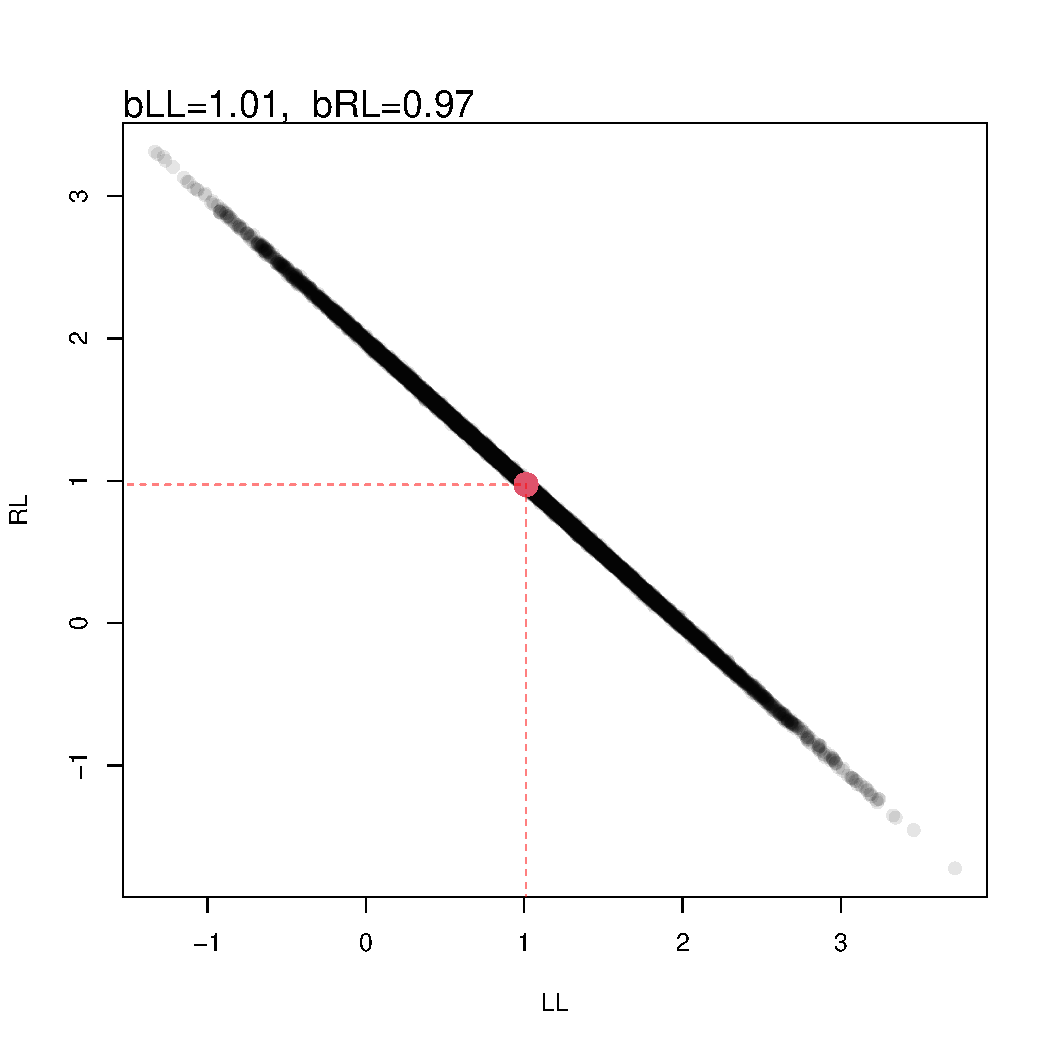
\includegraphics[scale=0.4]{fork4_triptych.pdf}}]
	{So, what is going on then??}
	
	the estimated parameters under the second regression,
	%
	\begin{itemize}
		%
		\item are in a thin ridge \\
		$Cor(bLL, bRL) \approx -1$
		\item statistical model finds not only one solution (\alert{red dot}), the thin ridge implies there are \textcolor{blue}{infinite solutions} for the parameters,\\
		{\small (related to the singular matrix thing)}
		%
	\end{itemize}
	%
\end{lhframe}
%
%
\begin{lhframe}[rhgraphic={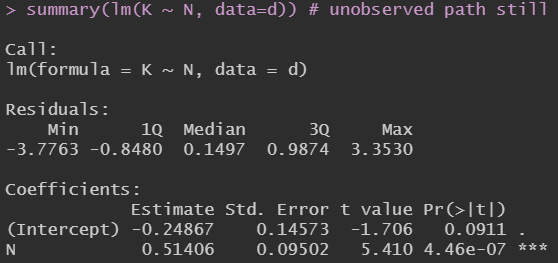
\includegraphics[scale=0.6]{fork4_reg1.png}}]
	{Not so great now??}
	
	based on \textcolor{blue}{DAG} and \textcolor{blue}{statistical analysis},
	%
	\begin{itemize}
		%
		\item the less biased and more precise model is the first, \\
		{\small \textcolor{blue}{(assuming our DAG is true)} }
		%
	\end{itemize}
	%
\end{lhframe}
%
%
%%%%%%%%%%%%%%%%%%%%%%%%%%%%%%%%%%%%%%%%%%%%%%%%%%%%%%%%%%%
\subsection{No more fork bias: neutral control}
%%%%%%%%%%%%%%%%%%%%%%%%%%%%%%%%%%%%%%%%%%%%%%%%%%%%%%%%%%%
%
%
\begin{frame}[t, negative]
	\subsectionpage
\end{frame}
%
%
\begin{frame}
	{Neutral control\footnote{\citet{Cinelli_et_al_2021} (p. 4)}}
	%
	\begin{columns}
		%
		\begin{column}{0.5\textwidth}
			%
			also known as,
			%
			\begin{itemize}
				%
				\item precision ``booster"
				\item similar to \textcolor{blue}{experimental design}
				%
			\end{itemize}
			
			research question, 
			%
			\begin{itemize}
				%
				\item \textcolor{blue}{Should we include $G$ on our model?}
				%
			\end{itemize}
			
			variables,
			%
			\begin{itemize}
				%
				\item A, ``hearing" age
				\item G, gender
				\item $U_{X}$, unobservable (e.g. no idea yet)
				\item H, inverse logit of entropy\\
				{\small (approximate of speech intelligibility)}
				%
			\end{itemize}
			%
		\end{column}
		%
		\begin{column}{0.5\textwidth}  
			%
			\begin{equ}
				%
				M = \left\{ \begin{aligned} 
					G \leftarrow & \; f_{G}(U_{G}, U_{X}) \\
					A \leftarrow & \; f_{A}(U_{A}) \\
					H \leftarrow & \; f_{H}(A, G, U_{H}) \\
					U \sim & \; P(\pmb{U})
				\end{aligned} \right
				%
				\caption*{(a) structural model}
				%
			\end{equ}
			%
			\begin{figure}
				%
				\begin{tikzpicture}
					% nodes
					\node[formula] at (-2,0) {$U_{A}$};
					\node[formula] at (-1,-0.3) {$A$};
					\node[formula] at (-1,1.5) {$U_{X}$};
					\node[formula] at (1,1.5) {$U_{G}$};
					\node[formula] at (0,1.1) {$G$};
					\node[formula] at (2,0) {$U_{H}$};
					\node[formula] at (1,-0.3) {$H$};
					
					% paths
					\draw [{Circle [open]}-{latex}{Circle}](-1.7,0)--(-0.9,0); % Ua->A
					\draw [-{latex}](-0.9,0)--(0.9,0); % A->H
					\draw [{Circle [open]}-{latex}{Circle}](1.7,0)--(0.9,0); % Uh->H
					%\draw [-{latex}](-0.95,0.05)--(0,0.75);
					\draw [{Circle [color=red]}-{latex}](0,0.8)--(0.9,0.1); % G->H
					\draw [{Circle [open]}-{latex}](0.9,1.3)--(0.1,0.8); % Ug->G
					\draw [{Circle [open]}-{latex}](-1,1.25)--(0,0.8); % Ux->G
					
					% extra
					\node at (0,-0.25) {$(?)$}; % symbol
				\end{tikzpicture}
				%
				\caption*{(b) causal diagram}
				%
			\end{figure}
			%
		\end{column}
		%
	\end{columns}
	%
\end{frame}
%
%
\begin{frame}
	{Simulation setting}
	%
	\begin{columns}
		%
		\begin{column}{0.5\textwidth}
			%
			\begin{figure}
				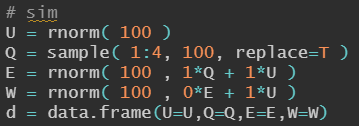
\includegraphics[scale=0.8]{fork5_code.png}
				\caption*{(c) R code}
			\end{figure}
			%
			\textcolor{blue}{Implications},
			%
			\begin{itemize}
				\item \dsep{A}{G} \\
				\item \ndsep{A}{H} \\
				\item \ndsep{G}{H} \\
			\end{itemize}
			%
		\end{column}
		%
		\begin{column}{0.5\textwidth}  
			%
			\begin{equ}
				%
				M = \left\{ \begin{aligned} 
					G \leftarrow & \; f_{G}(U_{G}) \\
					A \leftarrow & \; f_{A}(U_{A}) \\
					H \leftarrow & \; f_{H}(A, G, U_{H}) \\
					U \sim & \; P(\pmb{U})
				\end{aligned} \right
				%
				\caption*{(a) structural model}
				%
			\end{equ}
			%
			\begin{figure}
				%
				\begin{tikzpicture}
					% nodes
					\node[formula] at (-2,0) {$U_{A}$};
					\node[formula] at (-1,-0.3) {$A$};
					%\node[formula] at (-1,1.5) {$U_{X}$};
					\node[formula] at (1,1.5) {$U_{G}$};
					\node[formula] at (0,1.1) {$G$};
					\node[formula] at (2,0) {$U_{H}$};
					\node[formula] at (1,-0.3) {$H$};
					
					% paths
					\draw [{Circle [open]}-{latex}{Circle}](-1.7,0)--(-0.9,0); % Ua->A
					\draw [-{latex}](-0.9,0)--(0.9,0); % A->H
					\draw [{Circle [open]}-{latex}{Circle}](1.7,0)--(0.9,0); % Uh->H
					%\draw [-{latex}](-0.95,0.05)--(0,0.75);
					\draw [{Circle [color=red]}-{latex}](0,0.8)--(0.9,0.1); % G->H
					\draw [{Circle [open]}-{latex}](0.9,1.3)--(0.1,0.8); % Ug->G
					%\draw [{Circle [open]}-{latex}](-1,1.25)--(0,0.8); % Ux->G
				\end{tikzpicture}
				%
				\caption*{(b) causal diagram}
				%
			\end{figure}
			%
		\end{column}
		%
	\end{columns}
	%
\end{frame}
%
%
\begin{lhframe}[rhgraphic={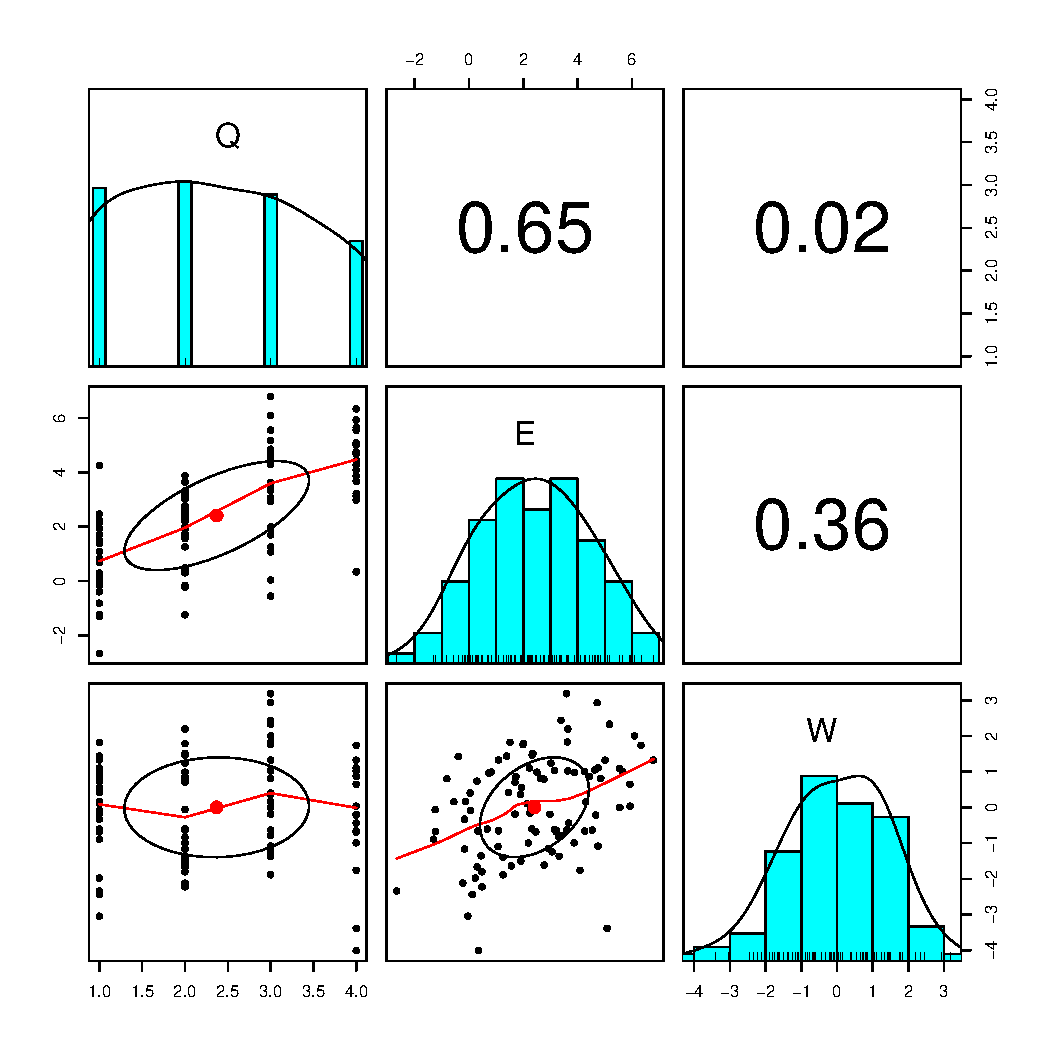
\includegraphics[scale=0.4]{fork5_panel.pdf}}]
	{``Eyeballing" analysis}
	
	based on \textcolor{blue}{correlation analysis},
	%
	\begin{itemize}
		%
		\item $cor(G, H)<0$, $cor(G, A) \approx 0$ and $cor(A, H) < 0$ goes in line of our ``rudimentary" understanding of the data.
		%
		\item we \textcolor{blue}{include both} as a covariate in our statistical model
		%
	\end{itemize}
	%
\end{lhframe}
%
%
\begin{lhframe}[rhgraphic={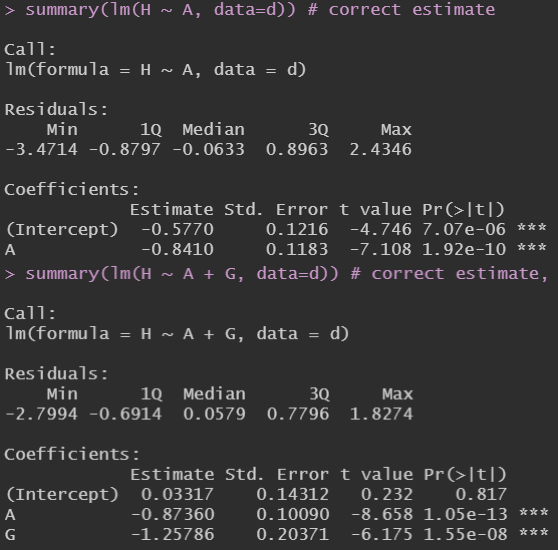
\includegraphics[scale=0.3]{fork5_reg.png}}]
	{Regression, regression!!}
	
	based on \textcolor{blue}{statistical analysis},
	%
	\begin{itemize}
		%
		\item almost no change on our estimates,
		\item lower standard errors for $A$ when $G$ is included \\
		{\small (because we have explained some variability in $H$, not related to $A$)}
		%
	\end{itemize}
	%
\end{lhframe}
%
%
\begin{lhframe}[rhgraphic={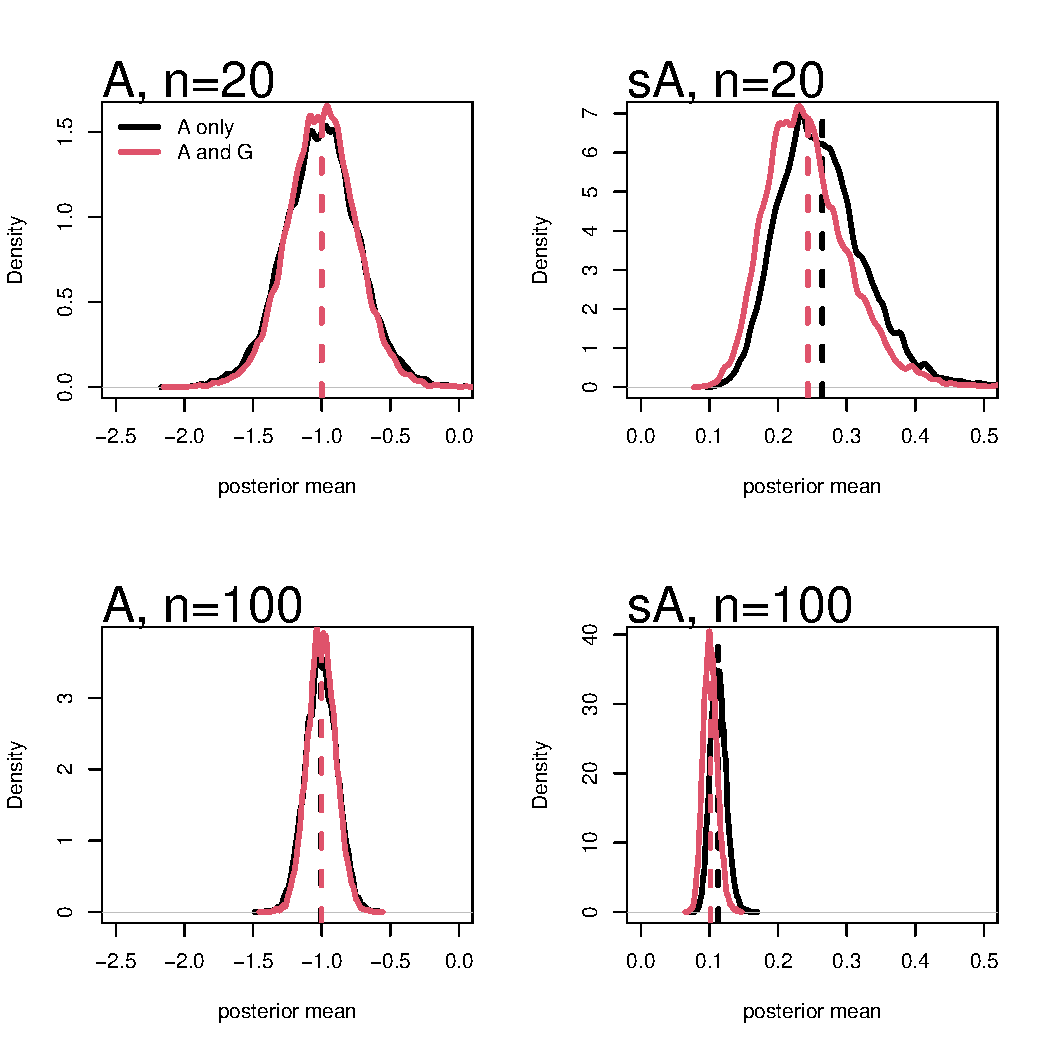
\includegraphics[scale=0.45]{fork5_samplesize.pdf}}]
	{I'll get more data!!}
	
	imagine we can continue sampling,
	%
	\begin{itemize}
		%
		\item top: $10,000$ samples $n=20$
		\item bottom: $10,000$ samples $n=100$
		%
	\end{itemize}
	
	under the \textcolor{blue}{second model}, \\
	the larger the sample size,
	%
	\begin{itemize}
		%
		\item the more \textcolor{blue}{certain} you are about your \textcolor{blue}{non-biased} estimates \\
		{\small (under the any model)}
		%
	\end{itemize}
	%
\end{lhframe}
%
%
%%%%%%%%%%%%%%%%%%%%%%%%%%%%%%%%%%%%%%%%%%%%%%%%%%%%%%%%%%%
\subsection{Pipe bias: precision parasite}
%%%%%%%%%%%%%%%%%%%%%%%%%%%%%%%%%%%%%%%%%%%%%%%%%%%%%%%%%%%
%
%
\begin{frame}[t, negative]
	\subsectionpage
\end{frame}
%
%
\begin{frame}
	{Precision parasite\footnote{\citet{McElreath_2022}, lecture 6; \citet{Cinelli_et_al_2021} (p. 5)}}
	%
	\begin{columns}
		%
		\begin{column}{0.5\textwidth}
			%
			research question, 
			%
			\begin{itemize}
				%
				\item \textcolor{blue}{What is the effect of $X$ on $Y$?}
				\item Should we include $Z$ in the model?
				%
			\end{itemize}
			
			variables,
			%
			\begin{itemize}
				%
				\item Z, ``parent" of X
				\item X, exposure
				\item Y, outcome
				%
			\end{itemize}
			%
		\end{column}
		%
		\begin{column}{0.5\textwidth}  
			%
			\begin{equ}
				%
				M = \left\{ \begin{aligned} 
					Z \leftarrow & \; f_{Z}(U_{Z}) \\
					X \leftarrow & \; f_{X}(Z, U_{X}) \\
					Y \leftarrow & \; f_{Y}(X, U_{Y}) \\
					U \sim & \; P(\pmb{U})
				\end{aligned} \right
				%
				\caption*{(a) structural model}
				%
			\end{equ}
			%
			\begin{figure}
				%
				\begin{tikzpicture}
					% nodes
					\node[formula] at (-2,0.8) {$U_{Z}$};
					\node[formula] at (-1,1) {$Z$};
					\node[formula] at (-2,0) {$U_{X}$};
					\node[formula] at (-1,-0.3) {$X$};
					\node[formula] at (1,-0.3) {$Y$};
					\node[formula] at (2,0) {$U_{Y}$};
					
					% paths
					\draw [{Circle [open]}-{latex}](-1.7,0.75)--(-1,0.75); % Uz->Z
					\draw [{Circle[color=red]}-{latex}](-0.95,0.8)--(-0.95,0.05); % Z->X
					\draw [{Circle [open]}-{latex}{Circle}](-1.7,0)--(-0.9,0); % Ux->X
					\draw [-{latex}](-0.9,0)--(0.9,0); % X->Y
					\draw [{Circle [open]}-{latex}{Circle}](1.7,0)--(0.9,0); % Uy->Y
					
					% extra
					\node at (0,-0.25) {$(?)$}; % symbol
				\end{tikzpicture}
				%
				\caption*{(b) causal diagram}
				%
			\end{figure}
			%
		\end{column}
		%
	\end{columns}
	%
\end{frame}
%
%
\begin{frame}
	{Simulation setting}
	%
	\begin{columns}
		%
		\begin{column}{0.5\textwidth}
			%
			\begin{figure}
				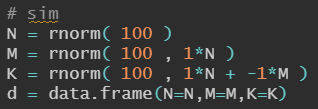
\includegraphics[scale=0.8]{pipe1_code.png}
				\caption*{(c) R code}
			\end{figure}
			%
			\textcolor{blue}{Implications},
			%
			\begin{itemize}
				\item \ndsep{X}{Y} \\
				\item \ndsep{Z}{Y} \; | X
			\end{itemize}
			%
		\end{column}
		%
		\begin{column}{0.5\textwidth}  
			%
			\begin{equ}
				%
				M = \left\{ \begin{aligned} 
					Z \leftarrow & \; f_{Z}(U_{Z}) \\
					X \leftarrow & \; f_{X}(Z, U_{X}) \\
					Y \leftarrow & \; f_{Y}(X, U_{Y}) \\
					U \sim & \; P(\pmb{U})
				\end{aligned} \right
				%
				\caption*{(a) structural model}
				%
			\end{equ}
			%
			\begin{figure}
				%
				\begin{tikzpicture}
					% nodes
					\node[formula] at (-2,0.8) {$U_{Z}$};
					\node[formula] at (-1,1) {$Z$};
					\node[formula] at (-2,0) {$U_{X}$};
					\node[formula] at (-1,-0.3) {$X$};
					\node[formula] at (1,-0.3) {$Y$};
					\node[formula] at (2,0) {$U_{Y}$};
					
					% paths
					\draw [{Circle [open]}-{latex}](-1.7,0.75)--(-1,0.75); % Uz->Z
					\draw [{Circle[color=red]}-{latex}](-0.95,0.8)--(-0.95,0.05); % Z->X
					\draw [{Circle [open]}-{latex}{Circle}](-1.7,0)--(-0.9,0); % Ux->X
					\draw [-{latex}](-0.9,0)--(0.9,0); % X->Y
					\draw [{Circle [open]}-{latex}{Circle}](1.7,0)--(0.9,0); % Uy->Y
				\end{tikzpicture}
				%
				\caption*{(b) causal diagram}
				%
			\end{figure}
			%
		\end{column}
		%
	\end{columns}
	%
\end{frame}
%
%
\begin{lhframe}[rhgraphic={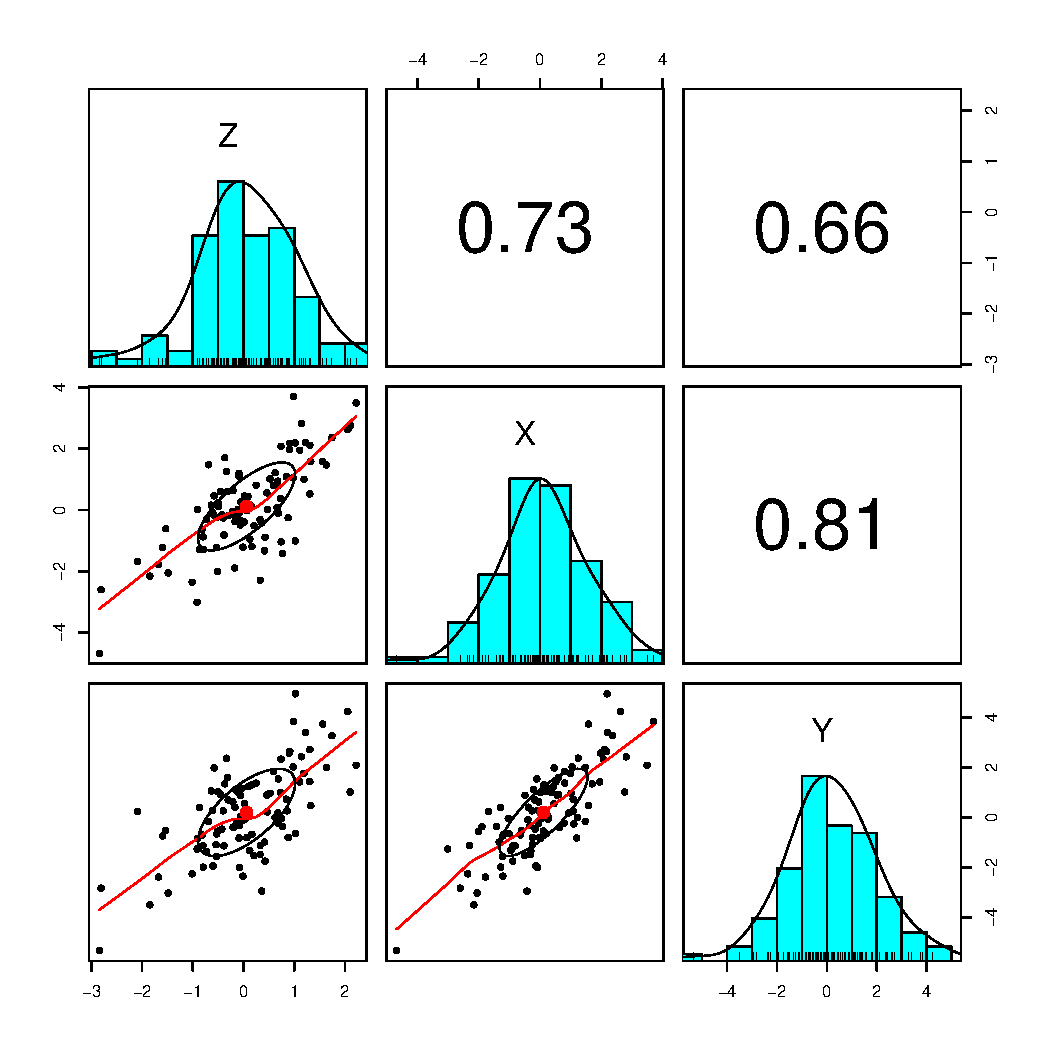
\includegraphics[scale=0.4]{pipe1_panel.pdf}}]
	{``Eyeballing" analysis}
	
	based on \textcolor{blue}{correlation analysis},
	%
	\begin{itemize}
		%
		\item $cor(Z, X)>0$ is not large enough to discard it as multicollinearity.
		%
		\item $cor(Z, Y)>0$ and $cor(X, Y)>0$ indicate \textcolor{blue}{both should be} in our model \\
		{\small (it might be our research hypothesis)}
		%
	\end{itemize}
	%
\end{lhframe}
%
%
\begin{lhframe}[rhgraphic={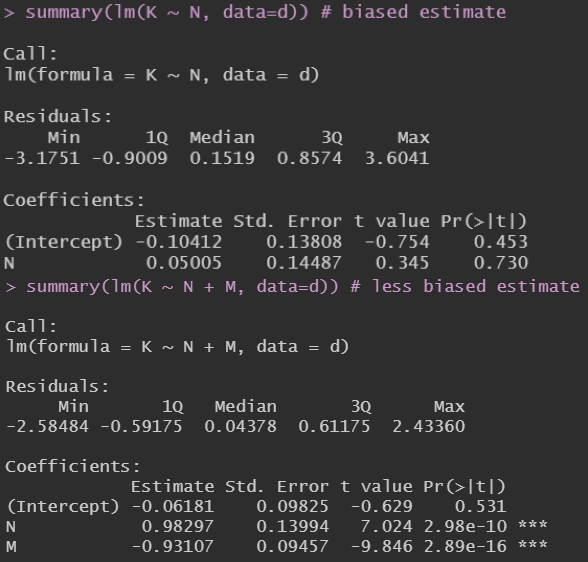
\includegraphics[scale=0.3]{pipe1_reg.png}}]
	{Regression, regression!!}
	
	based on \textcolor{blue}{statistical analysis},
	%
	\begin{itemize}
		%
		\item no bias in parameter if $Z$ is in,
		\item but we loose precision on $X$
		%
	\end{itemize}
	%
\end{lhframe}
%
%


\begin{lhframe}[rhgraphic={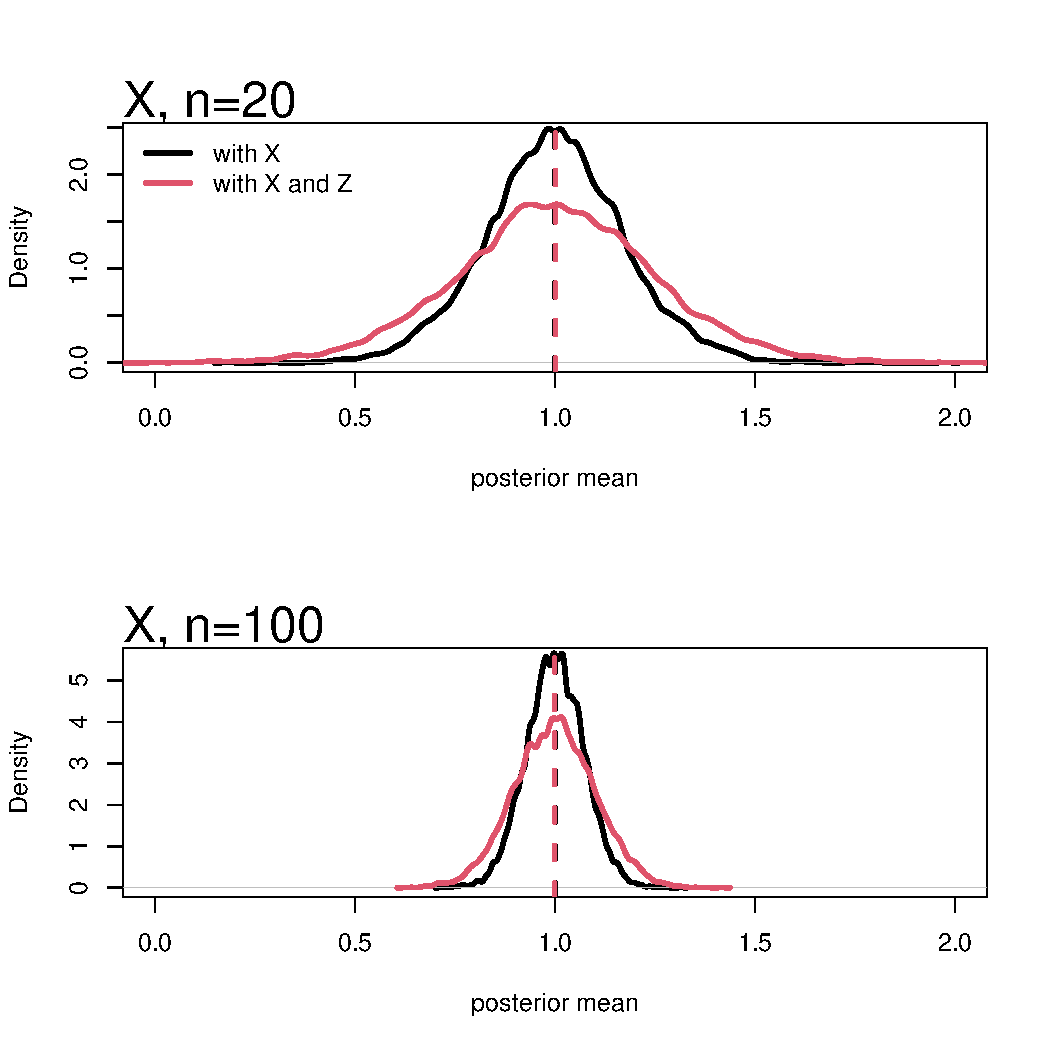
\includegraphics[scale=0.45]{pipe1_samplesize.pdf}}]
	{With more data??}
	
	imagine we can continue sampling,
	%
	\begin{itemize}
		%
		\item top: $10,000$ samples $n=20$
		\item bottom: $10,000$ samples $n=100$
		%
	\end{itemize}
	
	under the \textcolor{blue}{second model}, \\
	the larger the sample size,
	%
	\begin{itemize}
		%
		\item still \textcolor{blue}{less precise} estimates
		\item more \textcolor{blue}{difficult} to test hypothesis
		%
	\end{itemize}
	%
\end{lhframe}
%
%


\begin{frame}
	{Now, what is going on here??}
	%
	\begin{columns}
		%
		\begin{column}{0.5\textwidth}
			%
			based on \textcolor{blue}{DAG} and \textcolor{blue}{statistical model},
			%
			\begin{itemize}
				%
				\item conditioning on $Z$ reduces variation on $X$, leaving less variability that can explain outcome $Y$
				%
			\end{itemize}
			%
		\end{column}
		%
		\begin{column}{0.5\textwidth}  
			%
			\begin{equ}
				%
				M = \left\{ \begin{aligned} 
					Z \leftarrow & \; f_{Z}(U_{Z}) \\
					X \leftarrow & \; f_{X}(Z, U_{X}) \\
					Y \leftarrow & \; f_{Y}(X, U_{Y}) \\
					U \sim & \; P(\pmb{U})
				\end{aligned} \right
				%
				\caption*{(a) structural model}
				%
			\end{equ}
			%
			\begin{figure}
				%
				\begin{tikzpicture}
					% nodes
					\node[formula] at (-2,0.8) {$U_{Z}$};
					\node[formula] at (-1,1) {$Z$};
					\node[formula] at (-2,0) {$U_{X}$};
					\node[formula] at (-1,-0.3) {$X$};
					\node[formula] at (1,-0.3) {$Y$};
					\node[formula] at (2,0) {$U_{Y}$};
					
					% paths
					\draw [{Circle [open]}-{latex}](-1.7,0.75)--(-1,0.75); % Uz->Z
					\draw [{Circle[color=red]}-{latex}](-0.95,0.8)--(-0.95,0.05); % Z->X
					\draw [{Circle [open]}-{latex}{Circle}](-1.7,0)--(-0.9,0); % Ux->X
					\draw [-{latex}](-0.9,0)--(0.9,0); % X->Y
					\draw [{Circle [open]}-{latex}{Circle}](1.7,0)--(0.9,0); % Uy->Y
					
					% extra
					\node at (0,-0.25) {$(?)$}; % symbol
				\end{tikzpicture}
				%
				\caption*{(b) causal diagram}
				%
			\end{figure}
			%
		\end{column}
		%
	\end{columns}
	%
\end{frame}
%
%
\begin{lhframe}[rhgraphic={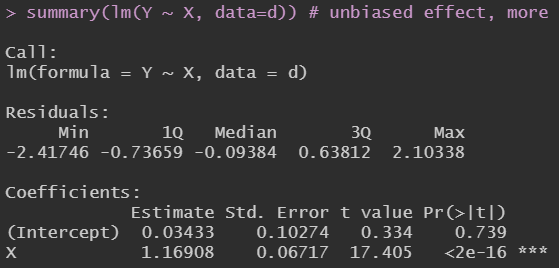
\includegraphics[scale=0.5]{pipe1_reg1.png}}]
	{Now, what is going on here??}
	
	based on \textcolor{blue}{DAG} and \textcolor{blue}{statistical analysis},
	%
	\begin{itemize}
		%
		\item the more appropriate model (for inference) is the first, \\
		{\small \textcolor{blue}{(assuming our DAG is true)} }
		%
	\end{itemize}
	%
\end{lhframe}
%
%
%%%%%%%%%%%%%%%%%%%%%%%%%%%%%%%%%%%%%%%%%%%%%%%%%%%%%%%%%%%
\subsection{Pipe bias: post-treatment}
%%%%%%%%%%%%%%%%%%%%%%%%%%%%%%%%%%%%%%%%%%%%%%%%%%%%%%%%%%%
%
%
\begin{frame}[t, negative]
	\subsectionpage
\end{frame}
%
%
\begin{frame}
	{Post-treatment bias\footnote{\citet{McElreath_2020}, chapter 6 (p. 170)}}
	%
	\begin{columns}
		%
		\begin{column}{0.5\textwidth}
			%
			case of,
			%
			\begin{itemize}
				%
				\item full mediation
				%
			\end{itemize}
			
			research question, 
			%
			\begin{itemize}
				%
				\item \textcolor{blue}{Does the treatment $T$ works?}
				%
			\end{itemize}
			
			variables,
			%
			\begin{itemize}
				%
				\item $H_{0}$, height of plant at $t=0$
				\item T, antifungal treatment
				\item F, presence of fungus
				\item $H_{1}$, height of plant at $t=1$ 
				%
			\end{itemize}
			%
		\end{column}
		%
		\begin{column}{0.5\textwidth}  
			%
			\begin{equ}
				%
				M = \left\{ \begin{aligned} 
					H_{0} \leftarrow & \; f_{H}(U_{H}) \\
					T \leftarrow & \; f_{T}(t) \\
					F \leftarrow & \; f_{F}(T, U_{F}) \\
					H_{1} \leftarrow & \; f_{H}(F,H_{0},U_{H}) \\
					U \sim & \; P(\pmb{U})
				\end{aligned} \right
				%
				\caption*{(a) structural model}
				%
			\end{equ}
			%
			\begin{figure}
				%
				\begin{tikzpicture}
					% nodes
					\node[formula] at (-2,0.8) {$t$};
					\node[formula] at (-1,1) {$T$};
					\node[formula] at (-2,0) {$U_{H}$};
					\node[formula] at (-1,-0.3) {$H_{0}$};
					\node[formula] at (1,1) {$U_{F}$};
					\node[formula] at (-0.1,1.05) {$F$};
					\node[formula] at (2,0) {$U_{H}$};
					\node[formula] at (1,-0.3) {$H_{1}$};
					
					% paths
					\draw [{Circle}-{latex}](-1.7,0.75)--(-1,0.75); % t->T
					\draw [{Circle}-{latex}](-1,0.75)--(0,0.75); % T->F
					\draw [{Circle [open]}-{latex}{Circle}](-1.7,0)--(-0.9,0); % Uh->Ho
					\draw [-{latex}](-0.9,0)--(0.9,0); % Ho->H1
					\draw [{Circle [open]}-{latex}{Circle}](1.7,0)--(0.9,0); % Uh->H1
					\draw [{Circle [open]}-{latex}](0.9,0.75)--(0.1,0.75); % Uf->F
					\draw [{Circle[color=red]}-{latex}](0,0.8)--(0.9,0.1); % F->H1
					
					% extra
					\node at (0,-0.25) {$(?)$}; % symbol
				\end{tikzpicture}
				%
				\caption*{(b) causal diagram}
				%
			\end{figure}
			%
		\end{column}
		%
	\end{columns}
	%
\end{frame}
%
%
\begin{frame}
	{Simulation setting}
	%
	\begin{columns}
		%
		\begin{column}{0.5\textwidth}
			%
			\begin{figure}
				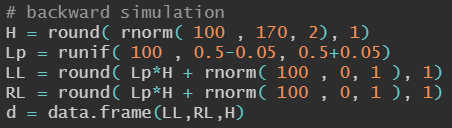
\includegraphics[scale=0.8]{pipe2_code.png}
				\caption*{(c) R code}
			\end{figure}
			%
			\textcolor{blue}{Implications},
			%
			\begin{itemize}
				\item \dsep{T}{$H_0$} \\
				\item \ndsep{T}{$H_1$} \\
				\item \ndsep{T}{$H_1$} \; | F
			\end{itemize}
			%
		\end{column}
		%
		\begin{column}{0.5\textwidth}  
			%
			\begin{equ}
				%
				M = \left\{ \begin{aligned} 
					H_{0} \leftarrow & \; f_{H}(U_{H}) \\
					T \leftarrow & \; f_{T}(t) \\
					F \leftarrow & \; f_{F}(T, U_{F}) \\
					H_{1} \leftarrow & \; f_{H}(F,H_{0},U_{H}) \\
					U \sim & \; P(\pmb{U})
				\end{aligned} \right
				%
				\caption*{(a) structural model}
				%
			\end{equ}
			%
			\begin{figure}
				%
				\begin{tikzpicture}
					% nodes
					\node[formula] at (-2,0.8) {$t$};
					\node[formula] at (-1,1) {$T$};
					\node[formula] at (-2,0) {$U_{H}$};
					\node[formula] at (-1,-0.3) {$H_{0}$};
					\node[formula] at (1,1) {$U_{F}$};
					\node[formula] at (-0.1,1.05) {$F$};
					\node[formula] at (2,0) {$U_{H}$};
					\node[formula] at (1,-0.3) {$H_{1}$};
					
					% paths
					\draw [{Circle}-{latex}](-1.7,0.75)--(-1,0.75); % t->T
					\draw [{Circle}-{latex}](-1,0.75)--(0,0.75); % T->F
					\draw [{Circle [open]}-{latex}{Circle}](-1.7,0)--(-0.9,0); % Uh->Ho
					\draw [-{latex}](-0.9,0)--(0.9,0); % Ho->H1
					\draw [{Circle [open]}-{latex}{Circle}](1.7,0)--(0.9,0); % Uh->H1
					\draw [{Circle [open]}-{latex}](0.9,0.75)--(0.1,0.75); % Uf->F
					\draw [{Circle[color=red]}-{latex}](0,0.8)--(0.9,0.1); % F->H1
				\end{tikzpicture}
				%
				\caption*{(b) causal diagram}
				%
			\end{figure}
			%
		\end{column}
		%
	\end{columns}
	%
\end{frame}
%
%
\begin{lhframe}[rhgraphic={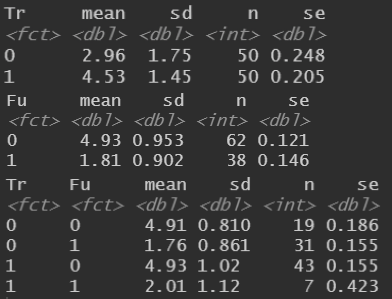
\includegraphics[scale=0.45]{pipe2_stat.png}}]
	{Descriptive analysis}
	
	based on \textcolor{blue}{descriptive analysis},
	%
	\begin{itemize}
		%
		\item \textcolor{blue}{positive change in height} with treatment.
		%
		\item \textcolor{blue}{negative change in height} with fungus.
		%
		\item \textcolor{blue}{diluted relationship} for $T$ when both are in the model \\
		{\small (hint: blocking path of information)}
		%
	\end{itemize}
	%
\end{lhframe}
%
%
\begin{lhframe}[rhgraphic={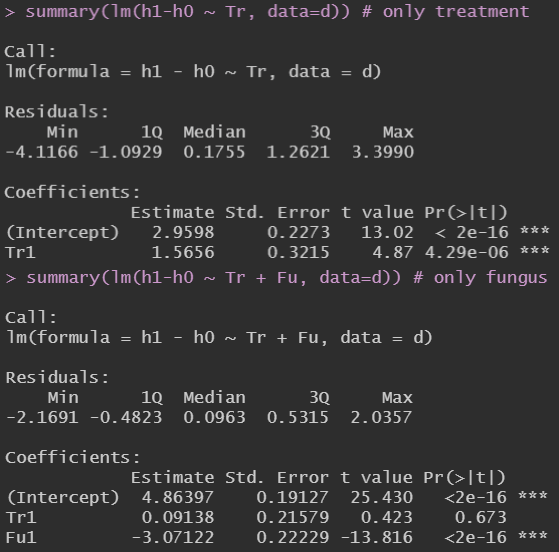
\includegraphics[scale=0.3]{pipe2_reg.png}}]
	{Again regression!!}
	
	based on \textcolor{blue}{statistical analysis} we have two different stories (but not quite),
	%
	\begin{itemize}
		%
		\item treatment has a \textcolor{blue}{significant effect},
		\item but gets completely diluted when fungus is considered in the model
		%
	\end{itemize}
	%
\end{lhframe}
%
%
\begin{lhframe}[rhgraphic={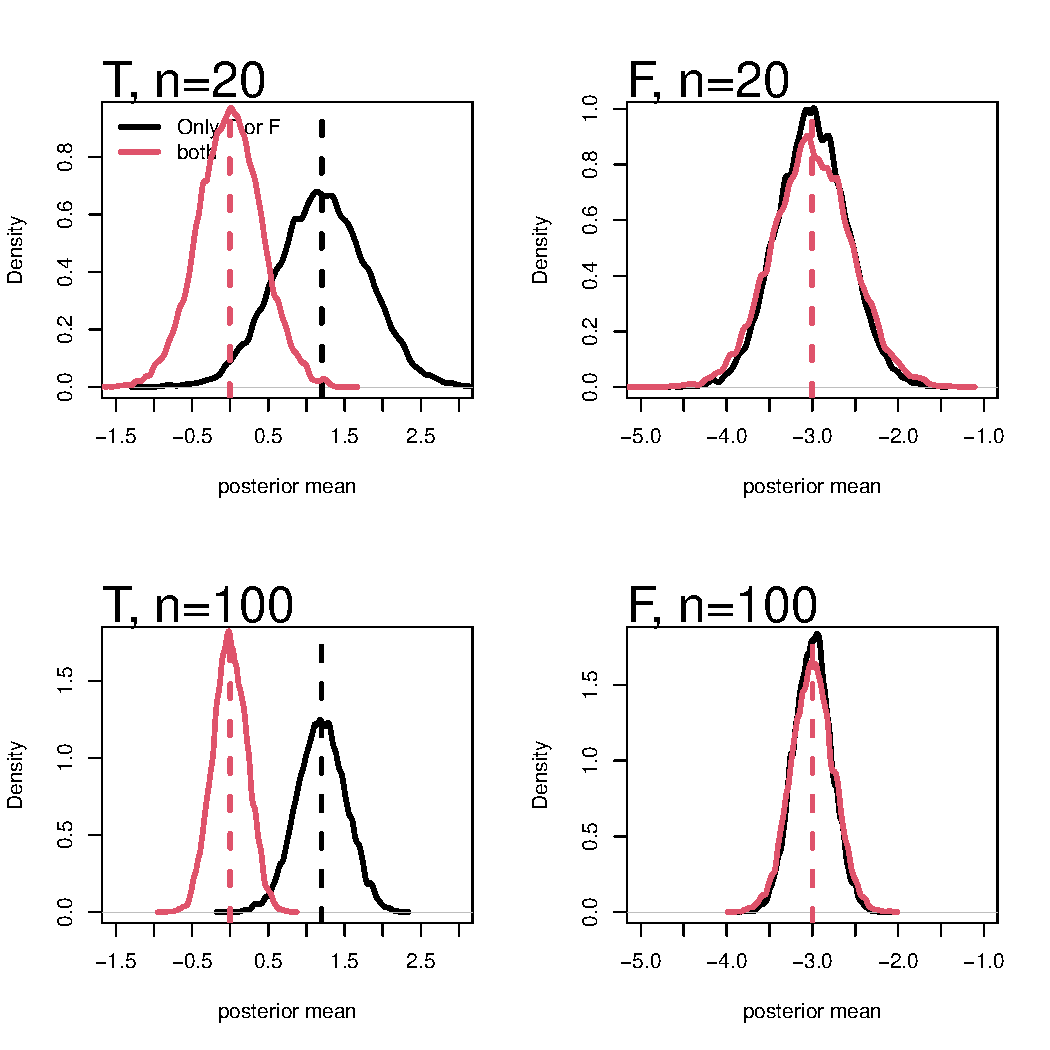
\includegraphics[scale=0.45]{pipe2_samplesize.pdf}}]
	{I can guess what happens with more data!!}
	
	imagine we can continue sampling,
	%
	\begin{itemize}
		%
		\item top: $10,000$ samples $n=20$
		\item bottom: $10,000$ samples $n=100$
		%
	\end{itemize}
	
	under the \textcolor{blue}{``incorrect" model}, \\
	the larger the sample size,
	%
	\begin{itemize}
		%
		\item the more \textcolor{blue}{certain} you are about your \textcolor{blue}{biased} $T$ estimates (not $F$)\\
		{\small (this result is not wrong!)}
		%
	\end{itemize}
	%
\end{lhframe}
%
%
\begin{frame}
	{The dream team!!}
	%
	\begin{columns}
		%
		\begin{column}{0.5\textwidth}
			%
			based on \textcolor{blue}{DAG} and \textcolor{blue}{statistical model},
			%
			\begin{itemize}
				%
				\item the 2nd D-separation states that if you to control any noncollider you block the \textcolor{blue}{backdoor path}, \\
				i.e. \dsep{T}{$H_1$} \; | F \\
				%
				\item therefore if we want to find if $T=1$ works, we \textcolor{blue}{should not} stratify by $F$
				%
			\end{itemize}
			%
		\end{column}
		%
		\begin{column}{0.5\textwidth}  
			%
			\begin{equ}
				%
				M = \left\{ \begin{aligned} 
					H_{0} \leftarrow & \; f_{H}(U_{H}) \\
					T \leftarrow & \; f_{T}(t) \\
					F \leftarrow & \; f_{F}(T, U_{F}) \\
					H_{1} \leftarrow & \; f_{H}(F,H_{0},U_{H}) \\
					U \sim & \; P(\pmb{U})
				\end{aligned} \right
				%
				\caption*{(a) structural model}
				%
			\end{equ}
			%
			\begin{figure}
				%
				\begin{tikzpicture}
					% nodes
					\node[formula] at (-2,0.8) {$t$};
					\node[formula] at (-1,1) {$T$};
					\node[formula] at (-2,0) {$U_{H}$};
					\node[formula] at (-1,-0.3) {$H_{0}$};
					\node[formula] at (1,1) {$U_{F}$};
					\node[formula] at (-0.1,1.05) {$F$};
					\node[formula] at (2,0) {$U_{H}$};
					\node[formula] at (1,-0.3) {$H_{1}$};
					
					% paths
					\draw [{Circle}-{latex}](-1.7,0.75)--(-1,0.75); % t->T
					\draw [{Circle}-{latex}](-1,0.75)--(0,0.75); % T->F
					\draw [{Circle [open]}-{latex}{Circle}](-1.7,0)--(-0.9,0); % Uh->Ho
					\draw [-{latex}](-0.9,0)--(0.9,0); % Ho->H1
					\draw [{Circle [open]}-{latex}{Circle}](1.7,0)--(0.9,0); % Uh->H1
					\draw [{Circle [open]}-{latex}](0.9,0.75)--(0.1,0.75); % Uf->F
					\draw [{Circle[color=red]}-{latex}](0,0.8)--(0.9,0.1); % F->H1
					
					% extra
					\node at (0,-0.25) {$(?)$}; % symbol
				\end{tikzpicture}
				%
				\caption*{(b) causal diagram}
				%
			\end{figure}
			%
		\end{column}
		%
	\end{columns}
	%
\end{frame}
%
%
\begin{lhframe}[rhgraphic={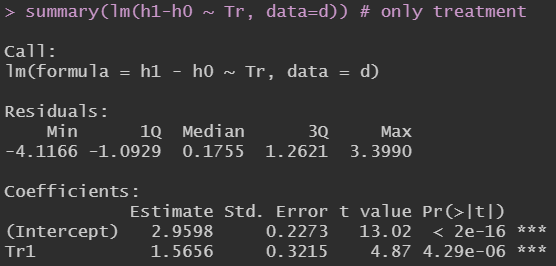
\includegraphics[scale=0.5]{pipe2_reg1.png}}]
	{the dream team!!}
	
	based on \textcolor{blue}{DAG} and \textcolor{blue}{statistical analysis},
	%
	\begin{itemize}
		%
		\item the model that answers our research question is the first one, \\
		{\small \textcolor{blue}{(assuming our DAG is true)} }
		%
	\end{itemize}
	%
\end{lhframe}
%
%
%%%%%%%%%%%%%%%%%%%%%%%%%%%%%%%%%%%%%%%%%%%%%%%%%%%%%%%%%%%
\subsection{Pipe bias: Simpson's paradox}
%%%%%%%%%%%%%%%%%%%%%%%%%%%%%%%%%%%%%%%%%%%%%%%%%%%%%%%%%%%
%
%
\begin{frame}[t, negative]
	\subsectionpage
\end{frame}
%
%
\begin{frame}
	{Masked relationships\footnote{\citet{McElreath_2020}, chapter 06 (p. 170)}}
	%
	\begin{columns}
		%
		\begin{column}{0.5\textwidth}
			%
			also known as,
			%
			\begin{itemize}
				%
				\item mediation
				\item masked relationships
				\item an instance of \textcolor{blue}{pipe bias}
				%
			\end{itemize}
			
			research question, 
			%
			\begin{itemize}
				%
				\item \textcolor{blue}{Does $N$ has a (direct) effect on $K$?}
				%
			\end{itemize}
			
			variables,
			%
			\begin{itemize}
				%
				\item M, mammal mass in kg.
				\item N, neocortex over total brain mass
				\item K, Kcal. per gram of milk
				%
			\end{itemize}
			%
		\end{column}
		%
		\begin{column}{0.5\textwidth}  
			%
			\begin{equ}
				%
				M = \left\{ \begin{aligned} 
					N \leftarrow & \; f_{N}(U_{N}) \\
					M \leftarrow & \; f_{M}(N,U_{M}) \\
					K \leftarrow & \; f_{K}(M, N, U_{K}) \\
					U \sim & \; P(\pmb{U})
				\end{aligned} \right
				%
				\caption*{(a) structural model}
				%
			\end{equ}
			%
			\begin{figure}
				%
				\begin{tikzpicture}
					% nodes
					\node[formula] at (-2,0) {$U_{N}$};
					\node[formula] at (-1,-0.3) {$N$};
					\node[formula] at (1,1.5) {$U_{M}$};
					\node[formula] at (0,1) {$M$};
					\node[formula] at (2,0) {$U_{K}$};
					\node[formula] at (1,-0.3) {$K$};
					
					% paths
					\draw [{Circle [open]}-{latex}{Circle}](-1.7,0)--(-0.9,0); % Un->N
					\draw [-{latex}](-0.9,0)--(0.9,0); % N->K
					\draw [{Circle [open]}-{latex}{Circle}](1.7,0)--(0.9,0); % Uk->K
					\draw [-{latex}](-0.95,0.05)--(0,0.75); % N->M
					\draw [{Circle [color=red]}-{latex}](0,0.8)--(0.9,0.1); % M->K
					\draw [{Circle [open]}-{latex}](0.9,1.3)--(0.1,0.8); % Um->M
					
					% extra
					\node at (0,-0.25) {$(?)$}; % symbol
				\end{tikzpicture}
				%
				\caption*{(b) causal diagram}
				%
			\end{figure}
			%
		\end{column}
		%
	\end{columns}
	%
\end{frame}
%
%
\begin{frame}
	{Simulation setting}
	%
	\begin{columns}
		%
		\begin{column}{0.5\textwidth}
			%
			\begin{figure}
				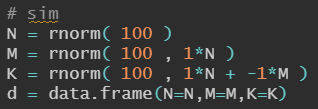
\includegraphics[scale=0.8]{pipe3_code.png}
				\caption*{(c) R code}
			\end{figure}
			%
			\textcolor{blue}{Implications},
			%
			\begin{itemize}
				\item \ndsep{N}{K} \\
				\item \ndsep{N}{K} \; | M
			\end{itemize}
			%
		\end{column}
		%
		\begin{column}{0.5\textwidth}  
			%
			\begin{equ}
				%
				M = \left\{ \begin{aligned} 
					N \leftarrow & \; f_{N}(U_{N}) \\
					M \leftarrow & \; f_{M}(M,U_{M}) \\
					K \leftarrow & \; f_{K}(M, N, U_{K}) \\
					U \sim & \; P(\pmb{U})
				\end{aligned} \right
				%
				\caption*{(a) structural model}
				%
			\end{equ}
			%
			\begin{figure}
				%
				\begin{tikzpicture}
					% nodes
					\node[formula] at (-2,0) {$U_{N}$};
					\node[formula] at (-1,-0.3) {$N$};
					\node[formula] at (1,1.5) {$U_{M}$};
					\node[formula] at (0,1) {$M$};
					\node[formula] at (2,0) {$U_{K}$};
					\node[formula] at (1,-0.3) {$K$};
					
					% paths
					\draw [{Circle [open]}-{latex}{Circle}](-1.7,0)--(-0.9,0); % Un->N
					\draw [-{latex}](-0.9,0)--(0.9,0); % N->K
					\draw [{Circle [open]}-{latex}{Circle}](1.7,0)--(0.9,0); % Uk->K
					\draw [-{latex}](-0.95,0.05)--(0,0.75); % N->M
					\draw [{Circle [color=red]}-{latex}](0,0.8)--(0.9,0.1); % M->K
					\draw [{Circle [open]}-{latex}](0.9,1.3)--(0.1,0.8); % Um->M
				\end{tikzpicture}
				%
				\caption*{(b) causal diagram}
				%
			\end{figure}
			%
		\end{column}
		%
	\end{columns}
	%
\end{frame}
%
%
\begin{lhframe}[rhgraphic={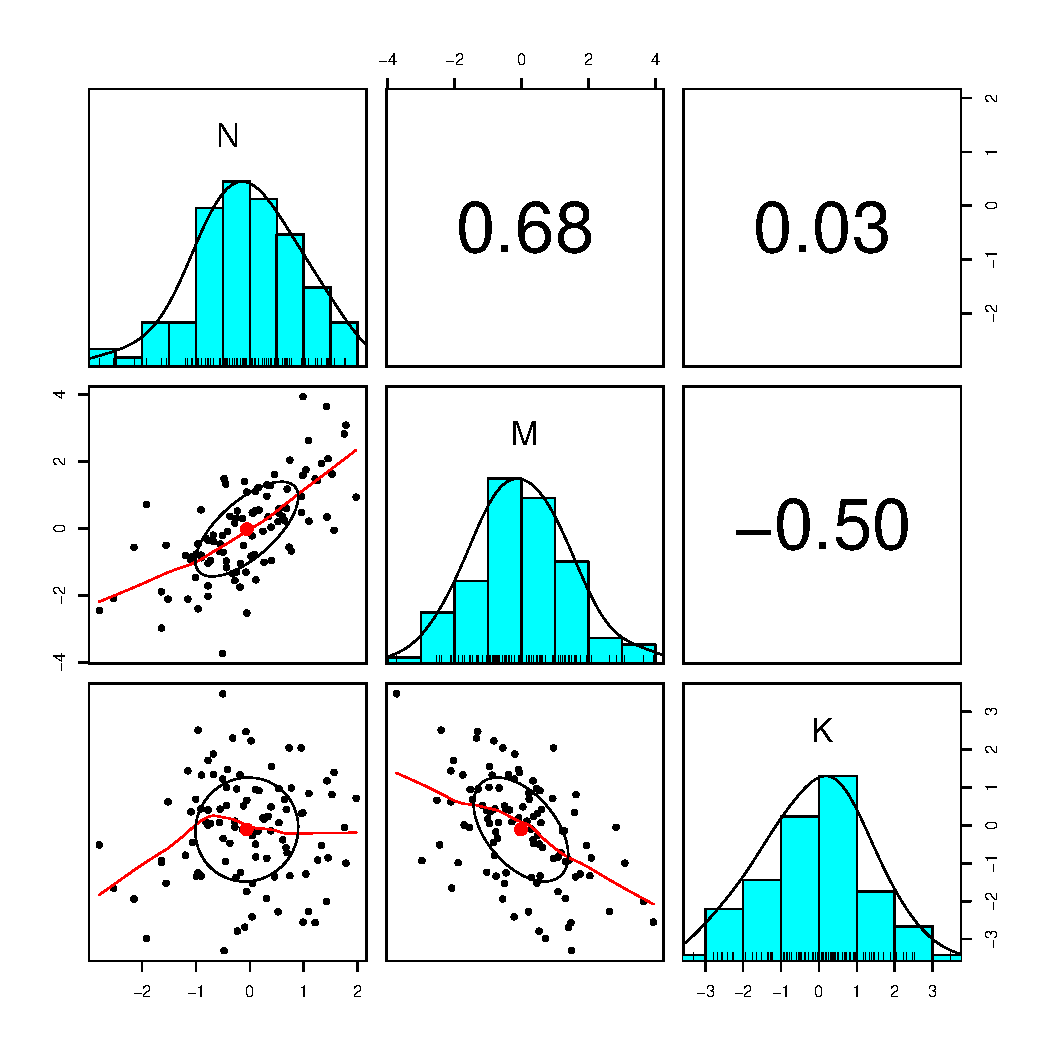
\includegraphics[scale=0.4]{pipe3_panel.pdf}}]
	{``Eyeballing" analysis}
	
	based on \textcolor{blue}{correlation analysis},
	%
	\begin{itemize}
		%
		\item $cor(M, K)<0$ does NOT goes in line of our ``rudimentary" understanding of the data.
		%
		\item and why there is $cor(N, K) \approx 0$? \\
		{\small (hint: univariate correlation)}
		%
		\item we \textcolor{blue}{include} $N$ as a covariate in our statistical model \\
		{\small (is our research hypothesis)}
		%
	\end{itemize}
	%
\end{lhframe}
%
%
\begin{lhframe}[rhgraphic={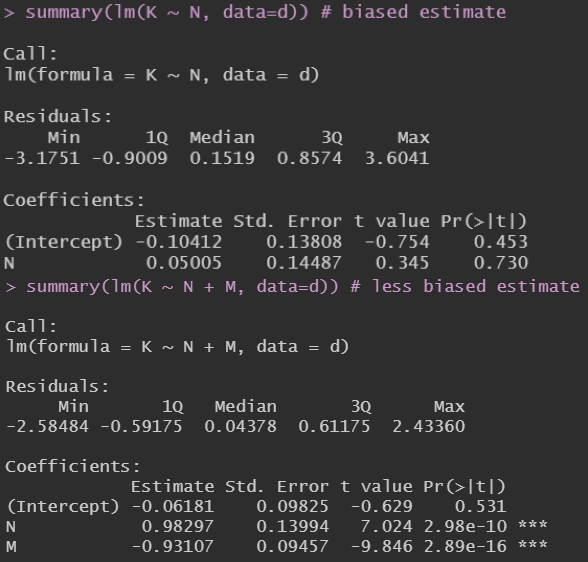
\includegraphics[scale=0.3]{pipe3_reg.png}}]
	{Regression, regression!!}
	
	based on \textcolor{blue}{statistical analysis},
	%
	\begin{itemize}
		%
		\item two regressions with two different results, which model is the ``true"?
		%
	\end{itemize}
	%
\end{lhframe}
%
%
\begin{lhframe}[rhgraphic={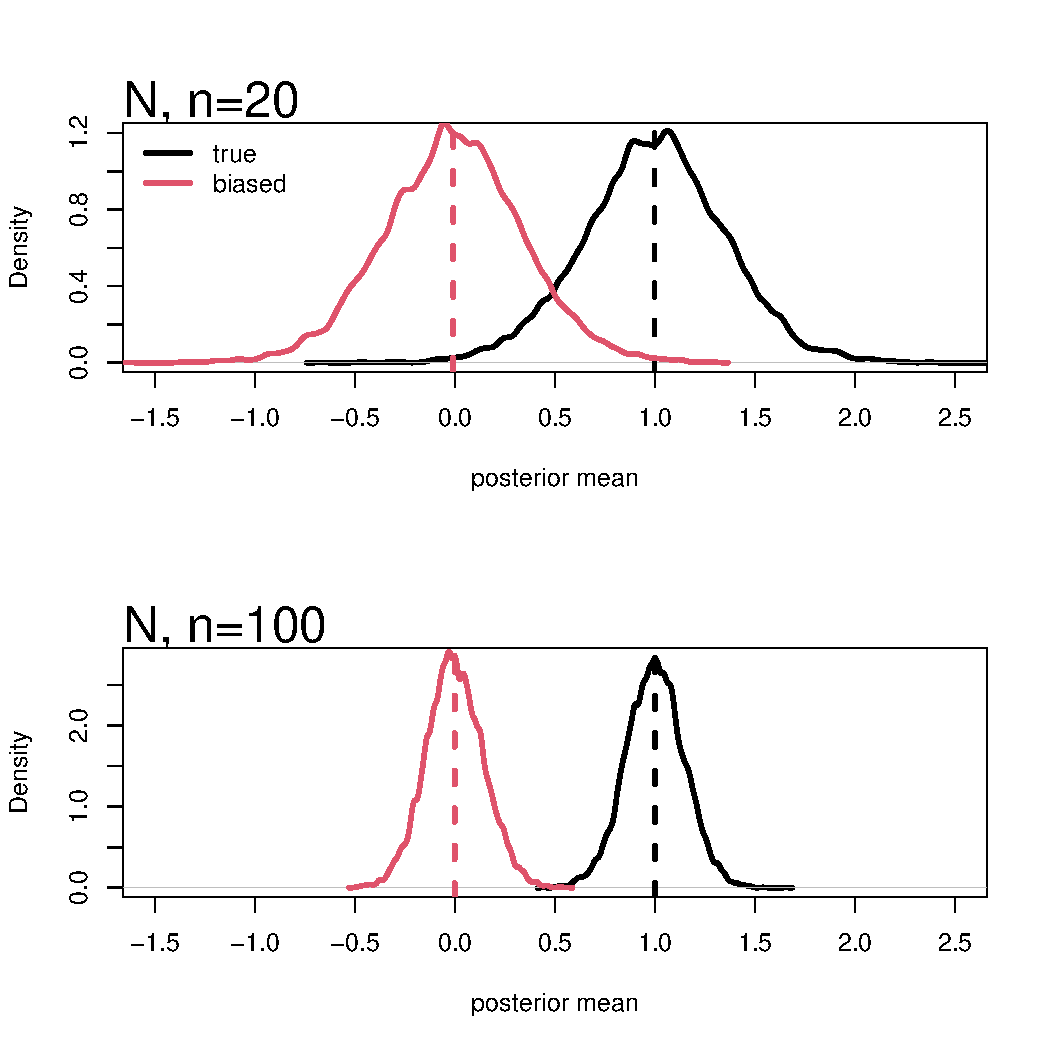
\includegraphics[scale=0.45]{pipe3_samplesize.pdf}}]
	{I'll get more data!!}
	
	imagine we can continue sampling,
	%
	\begin{itemize}
		%
		\item top: $10,000$ samples $n=20$
		\item bottom: $10,000$ samples $n=100$
		%
	\end{itemize}
	
	the larger the sample size,
	%
	\begin{itemize}
		%
		\item the more \textcolor{blue}{certain} you are about your estimates
		\item the more \textcolor{blue}{mistaken} you are about your research question \\
		{\small (under the ``incorrect" model)}
		%
	\end{itemize}
	%
\end{lhframe}
%
%
\begin{frame}
	{The dream team!!}
	%
	\begin{columns}
		%
		\begin{column}{0.5\textwidth}
			%
			based on \textcolor{blue}{DAG} and \textcolor{blue}{statistical model},
			%
			\begin{itemize}
				%
				\item the 2nd D-separation rule requires you to control any noncollider to block the \textcolor{blue}{backdoor path}, \\
				i.e. \ndsep{N}{K} \; | M \\
				%
				\item conditioning on $M$ we can find, \\
				{\small $E[K | do(n)] = E[\; E[K | N=n, M] \;]$} \\
				{\small (law of total expectation)}
				%
				\item then we can find the \\
				{\small $\text{ACE}(n) = E[D | do(n+1)] - E[D | do(n)]$ } \\
				{\small \textcolor{blue}{(Frisch-Waugh-Lovell theorem)} }
				%
			\end{itemize}
			%
		\end{column}
		%
		\begin{column}{0.5\textwidth}  
			%
			\begin{equ}
				%
				M = \left\{ \begin{aligned} 
					N \leftarrow & \; f_{N}(U_{N}) \\
					M \leftarrow & \; f_{M}(M,U_{M}) \\
					K \leftarrow & \; f_{K}(M, N, U_{K}) \\
					U \sim & \; P(\pmb{U})
				\end{aligned} \right
				%
				\caption*{(a) structural model}
				%
			\end{equ}
			%
			\begin{figure}
				%
				\begin{tikzpicture}
					% nodes
					\node[formula] at (-2,0) {$U_{N}$};
					\node[formula] at (-1,-0.3) {$N$};
					\node[formula] at (1,1.5) {$U_{M}$};
					\node[formula] at (0,1) {$M$};
					\node[formula] at (2,0) {$U_{K}$};
					\node[formula] at (1,-0.3) {$K$};
					
					% paths
					\draw [{Circle [open]}-{latex}{Circle}](-1.7,0)--(-0.9,0); % Un->N
					\draw [-{latex}](-0.9,0)--(0.9,0); % N->K
					\draw [{Circle [open]}-{latex}{Circle}](1.7,0)--(0.9,0); % Uk->K
					\draw [-{latex}](-0.95,0.05)--(0,0.75); % N->M
					\draw [{Circle [color=red]}-{latex}](0,0.8)--(0.9,0.1); % M->K
					\draw [{Circle [open]}-{latex}](0.9,1.3)--(0.1,0.8); % Um->M
					
					% extra
					\node at (0,-0.25) {$(?)$}; % symbol
				\end{tikzpicture}
				%
				\caption*{(b) causal diagram}
				%
			\end{figure}
			%
		\end{column}
		%
	\end{columns}
	%
\end{frame}
%
%
\begin{lhframe}[rhgraphic={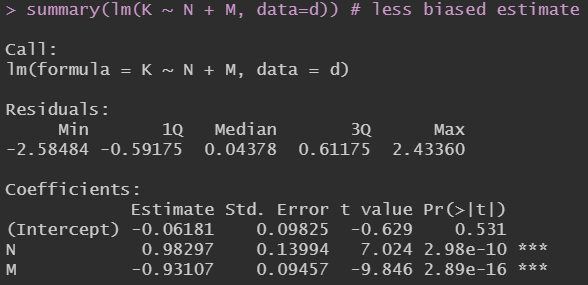
\includegraphics[scale=0.5]{pipe3_reg2.png}}]
	{the dream team!!}
	
	based on \textcolor{blue}{DAG} and \textcolor{blue}{statistical analysis},
	%
	\begin{itemize}
		%
		\item the less biased model is the second, \\
		{\small \textcolor{blue}{(assuming our DAG is true)} }
		%
	\end{itemize}
	%
\end{lhframe}
%
%
\begin{frame}
	{So, what is going on?}
	
	\begin{figure*}
		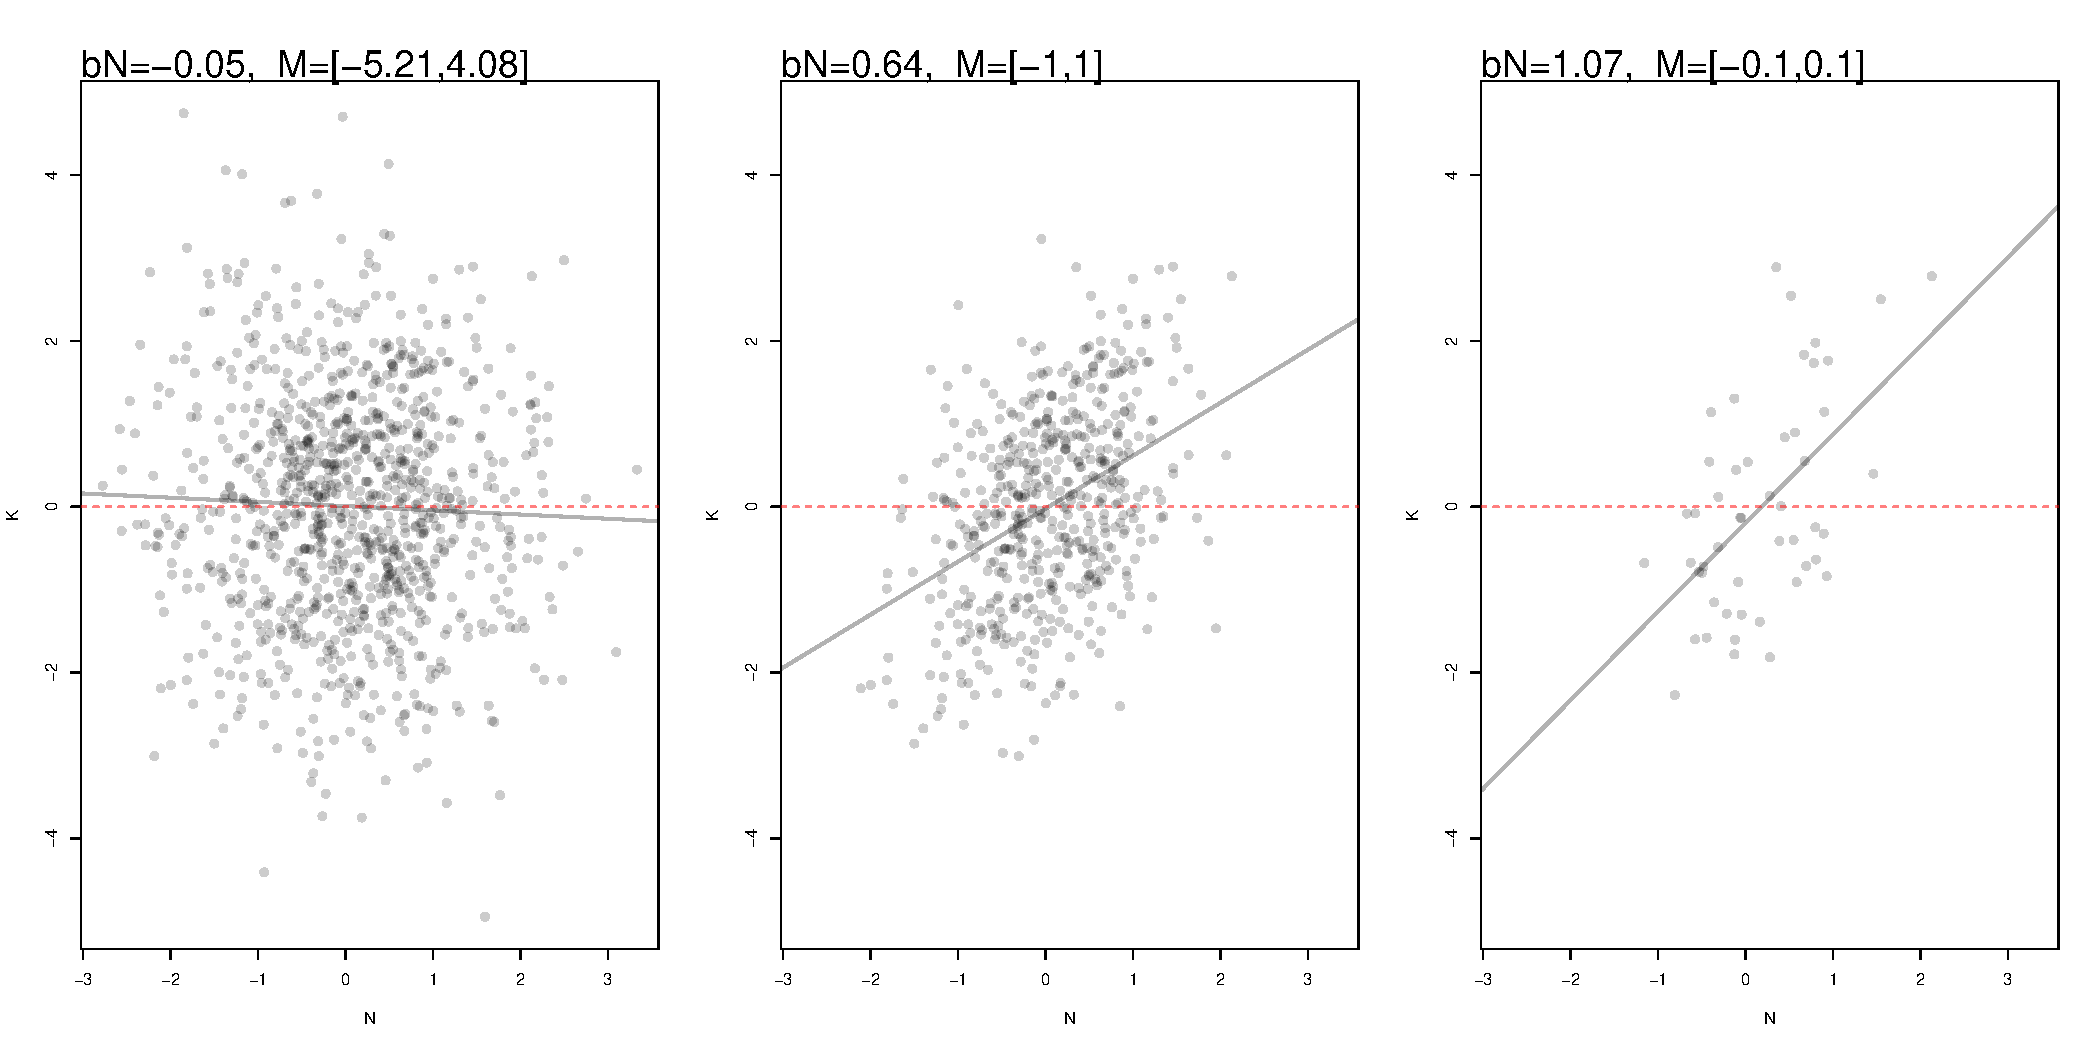
\includegraphics[width=\linewidth]{pipe3_triptych.pdf}
	\end{figure*}
	%
\end{frame}
%
%
\begin{frame}
	{Similar case, gender discrimination\footnote{\citet{McElreath_2020}, chapter 11 (p. 340)}}
	%
	\begin{columns}
		%
		\begin{column}{0.5\textwidth}
			%
			research question, 
			%
			\begin{itemize}
				%
				\item \textcolor{blue}{Do females are discriminated in school admissions, i.e. does $G \rightarrow A$?}
				%
			\end{itemize}
			
			variables,
			%
			\begin{itemize}
				%
				\item G, gender
				\item D, department of application
				\item A, admission
				%
			\end{itemize}
			%
			
			then,
			%
			\begin{itemize}
				%
				\item stratification by $D$ close mediation path (backdoor path on $A$)
				\item not stratifying by $D$ finds the \textcolor{blue}{total effect} of $G$ on $A$ (all paths) \\
				{\small (e.g. ``structural" discrimination)}
				%
			\end{itemize}
			%
		\end{column}
		%
		\begin{column}{0.5\textwidth}  
			%
			\begin{equ}
				%
				M = \left\{ \begin{aligned} 
					G \leftarrow & \; f_{G}(U_{G}) \\
					D \leftarrow & \; f_{D}(G,U_{D}) \\
					A \leftarrow & \; f_{A}(D, G, U_{A}) \\
					U \sim & \; P(\pmb{U})
				\end{aligned} \right
				%
				\caption*{(a) structural model}
				%
			\end{equ}
			%
			\begin{figure}
				%
				\begin{tikzpicture}
					% nodes
					\node[formula] at (-2,0) {$U_{G}$};
					\node[formula] at (-1,-0.3) {$G$};
					\node[formula] at (1,1.5) {$U_{D}$};
					\node[formula] at (0,1) {$D$};
					\node[formula] at (2,0) {$U_{A}$};
					\node[formula] at (1,-0.3) {$A$};
					
					% paths
					\draw [{Circle [open]}-{latex}{Circle}](-1.7,0)--(-0.9,0); % Ug->G
					\draw [-{latex}](-0.9,0)--(0.9,0); % G->A
					\draw [{Circle [open]}-{latex}{Circle}](1.7,0)--(0.9,0); % Ua->A
					\draw [-{latex}](-0.95,0.05)--(0,0.75); % G->D
					\draw [{Circle [color=red]}-{latex}](0,0.8)--(0.9,0.1); % D->A
					\draw [{Circle [open]}-{latex}](0.9,1.3)--(0.1,0.8); % Ud->D
					
					% extra
					\node at (0,-0.25) {$(?)$}; % symbol
				\end{tikzpicture}
				%
				\caption*{(b) causal diagram}
				%
			\end{figure}
			%
		\end{column}
		%
	\end{columns}
	%
\end{frame}
%
%
%%%%%%%%%%%%%%%%%%%%%%%%%%%%%%%%%%%%%%%%%%%%%%%%%%%%%%%%%%%
\subsection{No pipe/fork bias: good controls}
%%%%%%%%%%%%%%%%%%%%%%%%%%%%%%%%%%%%%%%%%%%%%%%%%%%%%%%%%%%
%
%
\begin{frame}[t, negative]
	\subsectionpage
\end{frame}
%
%
\begin{frame}
	{Pipe/fork good controls\footnote{\citet{Cinelli_et_al_2021} (p. 3)}}
	%
	\begin{columns}
		%
		\begin{column}{0.5\textwidth}
			%
			research question, 
			%
			\begin{itemize}
				%
				\item \textcolor{blue}{What is the (total) effect of $X$ on $Y$?} \\
				{\small (all directional paths from $X$ to $Y$)} \\
				{\small (i.e. no mediators)}
				%
			\end{itemize}
			
			variables,
			%
			\begin{itemize}
				%
				\item Z, confounder
				\item X, exposure
				\item M, mediator
				\item Y, outcome
				%
			\end{itemize}
			%
		\end{column}
		%
		\begin{column}{0.5\textwidth}  
			%
			\begin{equ}
				%
				M = \left\{ \begin{aligned} 
					Z \leftarrow & \; f_{Z}(U_{Z}) \\
					X \leftarrow & \; f_{X}(Z, U_{X}) \\
					M \leftarrow & \; f_{M}(X, Z, U_{M}) \\
					Y \leftarrow & \; f_{Y}(M, U_{Y}) \\
					U \sim & \; P(\pmb{U})
				\end{aligned} \right
				%
				\caption*{(a) structural model}
				%
			\end{equ}
			%
			\begin{figure}
				%
				\begin{tikzpicture}
					% nodes
					\node[formula] at (-2,0.8) {$U_{Z}$};
					\node[formula] at (-1,1) {$Z$};
					\node[formula] at (-2,0) {$U_{X}$};
					\node[formula] at (-1,-0.3) {$X$};
					\node[formula] at (1,1) {$U_{M}$};
					\node[formula] at (0,-0.3) {$M$};
					\node[formula] at (1,-0.3) {$Y$};
					\node[formula] at (2,0) {$U_{Y}$};
					
					% paths
					\draw [{Circle [open]}-{latex}](-1.7,0.75)--(-1,0.75); % Uz->Z
					\draw [{Circle[color=red]}-{latex}](-0.95,0.8)--(-0.95,0.05); % Z->X
					\draw [-{latex}](-0.90,0.75)--(-0.05,0.05); % Z->M
					\draw [{Circle [open]}-{latex}](-1.7,0)--(-1,0); % Ux->X
					\draw [{Circle}-{latex}](-1,0)--(-0.05,0); % X->M
					\draw [{Circle[open]}-{latex}](1,0.8)--(0,0.05); % Um->M
					\draw [{Circle}-{latex}](-0.05,0)--(0.9,0); % M->Y
					\draw [{Circle [open]}-{latex}{Circle}](1.7,0)--(0.9,0); % Uy->Y
					
					% extra
					\node at (-0.5,-0.25) {$(?)$}; % symbol
					\node at (0.5,-0.25) {$(?)$}; % symbol
				\end{tikzpicture}
				%
				\caption*{(b) causal diagram}
				%
			\end{figure}
			%
		\end{column}
		%
	\end{columns}
	%
\end{frame}
%
%
\begin{frame}
	{Simulation setting}
	%
	\begin{columns}
		%
		\begin{column}{0.5\textwidth}
			%
			\begin{figure}
				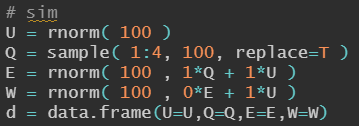
\includegraphics[scale=0.8]{pipefork1_code.png}
				\caption*{(c) R code}
			\end{figure}
			%
			\textcolor{blue}{Implications},
			%
			\begin{itemize}
				\item \ndsep{X}{M} \; | Z \\
				%
				\item \dsep{Z}{Y} \\
				%
			\end{itemize}
			%
		\end{column}
		%
		\begin{column}{0.5\textwidth}  
			%
			\begin{equ}
				%
				M = \left\{ \begin{aligned} 
					Z \leftarrow & \; f_{Z}(U_{Z}) \\
					X \leftarrow & \; f_{X}(Z, U_{X}) \\
					M \leftarrow & \; f_{M}(X, Z, U_{M}) \\
					Y \leftarrow & \; f_{Y}(M, U_{Y}) \\
					U \sim & \; P(\pmb{U})
				\end{aligned} \right
				%
				\caption*{(a) structural model}
				%
			\end{equ}
			%
			\begin{figure}
				%
				\begin{tikzpicture}
					% nodes
					\node[formula] at (-2,0.8) {$U_{Z}$};
					\node[formula] at (-1,1) {$Z$};
					\node[formula] at (-2,0) {$U_{X}$};
					\node[formula] at (-1,-0.3) {$X$};
					\node[formula] at (1,1) {$U_{M}$};
					\node[formula] at (0,-0.3) {$M$};
					\node[formula] at (1,-0.3) {$Y$};
					\node[formula] at (2,0) {$U_{Y}$};
					
					% paths
					\draw [{Circle [open]}-{latex}](-1.7,0.75)--(-1,0.75); % Uz->Z
					\draw [{Circle[color=red]}-{latex}](-0.95,0.8)--(-0.95,0.05); % Z->X
					\draw [-{latex}](-0.90,0.75)--(-0.05,0.05); % Z->M
					\draw [{Circle [open]}-{latex}{Circle}](-1.7,0)--(-0.9,0); % Ux->X
					%\draw [{Circle}-{latex}](-1,0)--(-0.05,0); % X->M
					\draw [{Circle[open]}-{latex}](1,0.8)--(0,0.05); % Um->M
					\draw [{Circle}-{latex}](-0.05,0)--(0.9,0); % M->Y
					\draw [{Circle [open]}-{latex}{Circle}](1.7,0)--(0.9,0); % Uy->Y
				\end{tikzpicture}
				%
				\caption*{(b) causal diagram}
				%
			\end{figure}
			%
		\end{column}
		%
	\end{columns}
	%
\end{frame}
%
%
\begin{lhframe}[rhgraphic={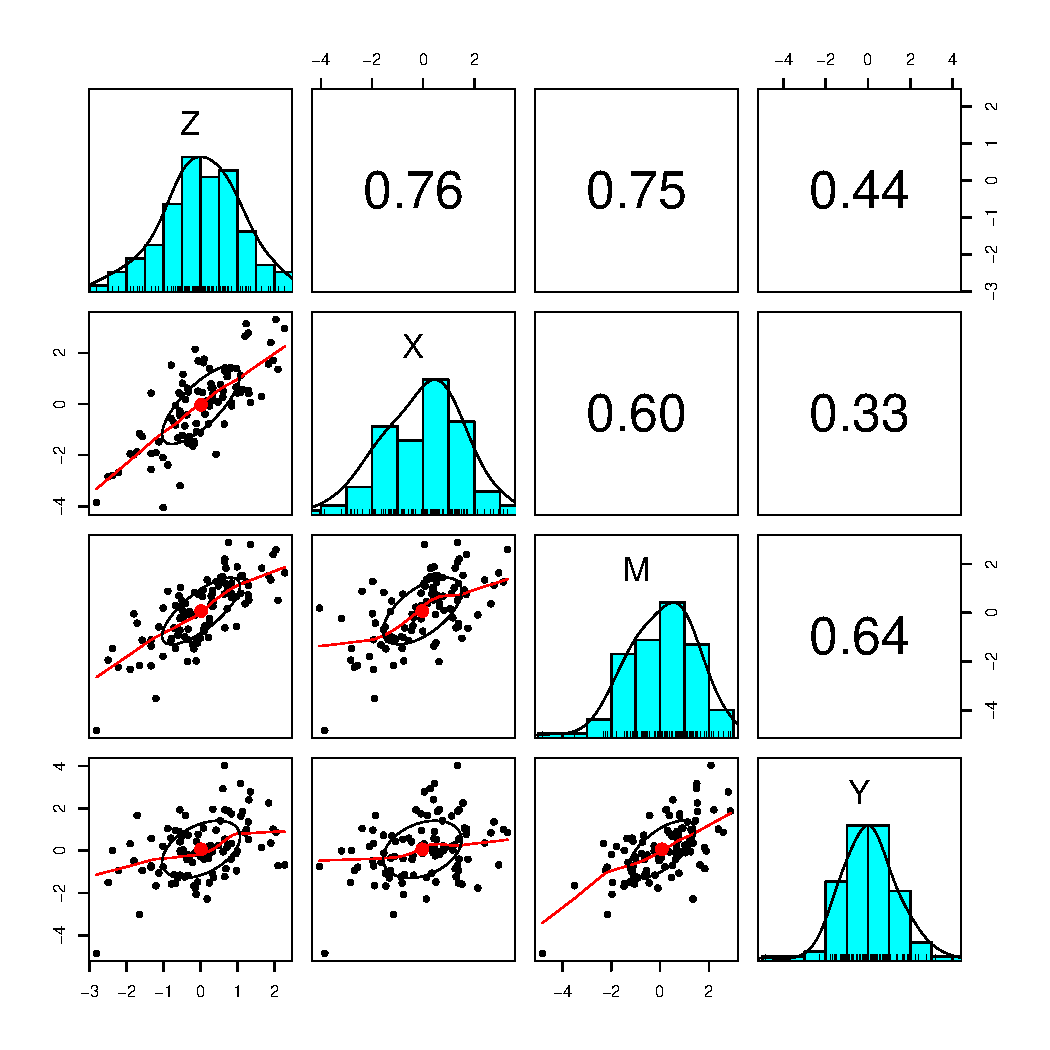
\includegraphics[scale=0.4]{pipefork1_panel.pdf}}]
	{``Eyeballing" analysis}
	
	based on \textcolor{blue}{correlation analysis},
	%
	\begin{itemize}
		%
		\item $X$ and $M$ should be in your model,\\
		{\small (but we know a full mediator closes the backdoor path, and \textcolor{blue}{we do not want that}: not our research question)}
		%
		\item while $cor(Z, M)\approx 0.8$ prevents from using $Z$ as a covariate \\
		{\small (possibly a multicollinearity problem)}
		%
		\item since we will not include $M$, now $Z$ can be included
		%
	\end{itemize}
	%
\end{lhframe}
%
%
\begin{lhframe}[rhgraphic={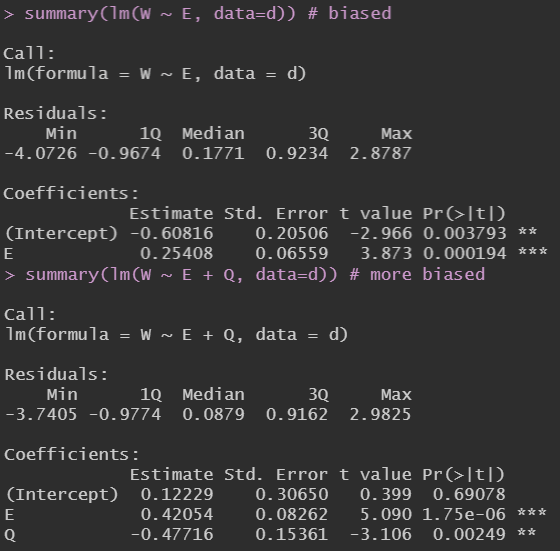
\includegraphics[scale=0.3]{pipefork1_reg.png}}]
	{Regression, regression!!}
	
	based on \textcolor{blue}{statistical analysis},
	%
	\begin{itemize}
		%
		\item two different stories
		\item in one $X$ has small but significant effect
		\item which model is the ``truth"?
		%
	\end{itemize}
	%
\end{lhframe}
%
%
\begin{lhframe}[rhgraphic={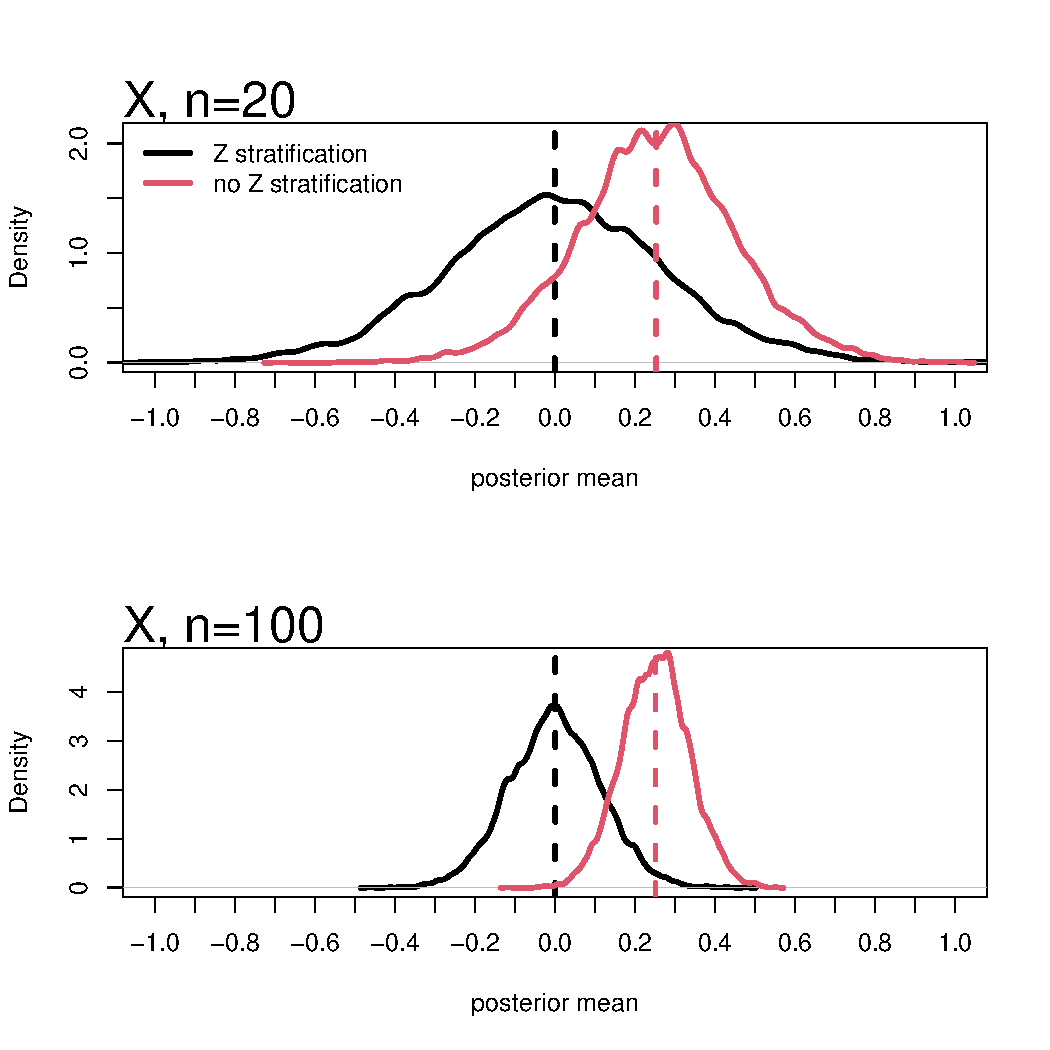
\includegraphics[scale=0.45]{pipefork1_samplesize.pdf}}]
	{the telled tell of more data!!}
	
	imagine we can continue sampling,
	%
	\begin{itemize}
		%
		\item top: $10,000$ samples $n=20$
		\item bottom: $10,000$ samples $n=100$
		%
	\end{itemize}
	
	under the \textcolor{blue}{incorrect model}, \\
	the larger the sample size,
	%
	\begin{itemize}
		%
		\item the more \textcolor{blue}{certain} you are about your \textcolor{blue}{biased} estimates
		%
	\end{itemize}
	%
\end{lhframe}
%
%
\begin{frame}
	{Yo, what is going on??}
	%
	\begin{columns}
		%
		\begin{column}{0.5\textwidth}
			%
			based on \textcolor{blue}{DAG} and \textcolor{blue}{statistical model},
			%
			\begin{itemize}
				%
				\item there are two paths from $X$ to $Y$\\
				$X \rightarrow M \rightarrow Y$ \\
				$X \rightarrow Z \rightarrow M \rightarrow Y$
				%
				\item stratifying by $Z$ closes the second, \\
				{\small (a confounder path)}
				%
				\item estimate $bZ$ corresponds to the \textcolor{blue}{total effect} of $Z$ on $Y$, \\
				i.e. $Z \rightarrow M \rightarrow Y$ \\
				{\small (but this is not our main research interest)}
				%
			\end{itemize}
			%
		\end{column}
		%
		\begin{column}{0.5\textwidth}  
			%
			\begin{equ}
				%
				M = \left\{ \begin{aligned} 
					Z \leftarrow & \; f_{Z}(U_{Z}) \\
					X \leftarrow & \; f_{X}(Z, U_{X}) \\
					M \leftarrow & \; f_{M}(X, Z, U_{M}) \\
					Y \leftarrow & \; f_{Y}(M, U_{Y}) \\
					U \sim & \; P(\pmb{U})
				\end{aligned} \right
				%
				\caption*{(a) structural model}
				%
			\end{equ}
			%
			\begin{figure}
				%
				\begin{tikzpicture}
					% nodes
					\node[formula] at (-2,0.8) {$U_{Z}$};
					\node[formula] at (-1,1) {$Z$};
					\node[formula] at (-2,0) {$U_{X}$};
					\node[formula] at (-1,-0.3) {$X$};
					\node[formula] at (1,1) {$U_{M}$};
					\node[formula] at (0,-0.3) {$M$};
					\node[formula] at (1,-0.3) {$Y$};
					\node[formula] at (2,0) {$U_{Y}$};
					
					% paths
					\draw [{Circle [open]}-{latex}](-1.7,0.75)--(-1,0.75); % Uz->Z
					\draw [{Circle[color=red]}-{latex}](-0.95,0.8)--(-0.95,0.05); % Z->X
					\draw [-{latex}](-0.90,0.75)--(-0.05,0.05); % Z->M
					\draw [{Circle [open]}-{latex}](-1.7,0)--(-1,0); % Ux->X
					\draw [{Circle}-{latex}](-1,0)--(-0.05,0); % X->M
					\draw [{Circle[open]}-{latex}](1,0.8)--(0,0.05); % Um->M
					\draw [{Circle}-{latex}](-0.05,0)--(0.9,0); % M->Y
					\draw [{Circle [open]}-{latex}{Circle}](1.7,0)--(0.9,0); % Uy->Y
					
					% extra
					\node at (-0.5,-0.25) {$(?)$}; % symbol
					\node at (0.5,-0.25) {$(?)$}; % symbol
				\end{tikzpicture}
				%
				\caption*{(b) causal diagram}
				%
			\end{figure}
			%
		\end{column}
		%
	\end{columns}
	%
\end{frame}
%
%
\begin{frame}
	{Similar cases\footnote{\citet{Cinelli_et_al_2021} (p. 3)}}
	%
	\begin{columns}
		%
		\begin{column}{0.5\textwidth}
			%
			research question, 
			%
			\begin{itemize}
				%
				\item \textcolor{blue}{What is the (total) effect of $X$ on $Y$?} \\
				{\small (all directional paths from $X$ to $Y$)} \\
				{\small (i.e. no mediators)}
				%
			\end{itemize}
			
			then,
			%
			\begin{itemize}
				%
				\item stratifying by $Z$ is still a good idea \\
				{\small ($U_{Z}$ is not draw out of convenience)}
				%
			\end{itemize}
			%
		\end{column}
		%
		\begin{column}{0.5\textwidth}  
			%
			\begin{figure}
				%
				\begin{tikzpicture}
					% nodes
					%\node[formula] at (-2,0.8) {$U_{Z}$};
					\node[formula] at (-1,1) {$Z$};
					\node[formula] at (-2,0) {$U_{X}$};
					\node[formula] at (-1,-0.3) {$X$};
					\node[formula] at (0,1) {$U_{K}$};
					\node[formula] at (1,1) {$U_{M}$};
					\node[formula] at (0,-0.3) {$M$};
					\node[formula] at (1,-0.3) {$Y$};
					\node[formula] at (2,0) {$U_{Y}$};
					
					% paths
					%\draw [{Circle [open]}-{latex}](-1.7,0.75)--(-1,0.75); % Uz->Z
					\draw [{Circle[color=red]}-{latex}](-0.95,0.8)--(-0.95,0.05); % Z->X
					\draw [{Circle [open]}-{latex}](-1.7,0)--(-1,0); % Ux->X
					\draw [{Circle}-{latex}](-1,0)--(-0.05,0); % X->M
					\draw [{Circle[open]}-{latex}](0.05,0.75)--(-0.9,0.75); % Uk->Z
					\draw [-{latex}](0,0.70)--(0,0.05); % Uk->M
					\draw [{Circle[open]}-{latex}](1,0.8)--(0,0.05); % Um->M
					\draw [{Circle}-{latex}](-0.05,0)--(0.9,0); % M->Y
					\draw [{Circle [open]}-{latex}{Circle}](1.7,0)--(0.9,0); % Uy->Y
					
					% extra
					\node at (-0.5,-0.25) {$(?)$}; % symbol
					\node at (0.5,-0.25) {$(?)$}; % symbol
				\end{tikzpicture}
				%
				\caption*{(b) causal diagram}
				%
			\end{figure}
			%
			%
			\begin{figure}
				%
				\begin{tikzpicture}
					% nodes
					%\node[formula] at (-2,0.8) {$U_{Z}$};
					\node[formula] at (-1,1) {$U_{K}$};
					\node[formula] at (-2,0) {$U_{X}$};
					\node[formula] at (-1,-0.3) {$X$};
					\node[formula] at (0,1) {$Z$};
					\node[formula] at (1,1) {$U_{M}$};
					\node[formula] at (0,-0.3) {$M$};
					\node[formula] at (1,-0.3) {$Y$};
					\node[formula] at (2,0) {$U_{Y}$};
					
					% paths
					%\draw [{Circle [open]}-{latex}](-1.7,0.75)--(-1,0.75); % Uz->Z
					\draw [{Circle[open]}-{latex}](-0.95,0.8)--(-0.95,0.05); % Uk->X
					\draw [{Circle [open]}-{latex}](-1.7,0)--(-1,0); % Ux->X
					\draw [{Circle}-{latex}](-1,0)--(-0.05,0); % X->M
					\draw [-{latex}](-0.9,0.75)--(-0.05,0.75); % Uk->Z
					\draw [{Circle[color=red]}-{latex}](0,0.8)--(0,0.05); % Z->M
					\draw [{Circle[open]}-{latex}](1,0.8)--(0,0.05); % Um->M
					\draw [{Circle}-{latex}](-0.05,0)--(0.9,0); % M->Y
					\draw [{Circle [open]}-{latex}{Circle}](1.7,0)--(0.9,0); % Uy->Y
					
					% extra
					\node at (-0.5,-0.25) {$(?)$}; % symbol
					\node at (0.5,-0.25) {$(?)$}; % symbol
				\end{tikzpicture}
				%
				\caption*{(b) causal diagram}
				%
			\end{figure}
			%
		\end{column}
		%
	\end{columns}
	%
\end{frame}
%
%
\begin{frame}
	{Careful what you control for (though)}
	%
	\begin{columns}
		%
		\begin{column}{0.5\textwidth}
			%
			\begin{figure}
				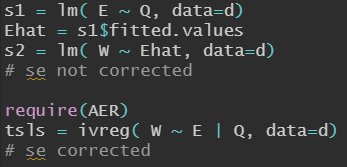
\includegraphics[scale=0.8]{pipefork1_code2.png}
				\caption*{(c) R code}
			\end{figure}
			%
			\textcolor{blue}{Implications},
			%
			\begin{itemize}
				\item \dsep{X}{Y} \\
				\item \dsep{Z}{Y} \\
				\item \ndsep{X}{M} \; | Z 
			\end{itemize}
			%
		\end{column}
		%
		\begin{column}{0.5\textwidth}  
			%
			\begin{equ}
				%
				M = \left\{ \begin{aligned} 
					Z \leftarrow & \; f_{Z}(U_{Z}) \\
					X \leftarrow & \; f_{X}(Z, U_{X}) \\
					M \leftarrow & \; f_{M}(X, Z, U_{M}) \\
					Y \leftarrow & \; f_{Y}(U_{Y}) \\
					U \sim & \; P(\pmb{U})
				\end{aligned} \right
				%
				\caption*{(a) structural model}
				%
			\end{equ}
			%
			\begin{figure}
				%
				\begin{tikzpicture}
					% nodes
					\node[formula] at (-2,0.8) {$U_{Z}$};
					\node[formula] at (-1,1) {$Z$};
					\node[formula] at (-2,0) {$U_{X}$};
					\node[formula] at (-1,-0.3) {$X$};
					\node[formula] at (1,1) {$U_{M}$};
					\node[formula] at (0,-0.3) {$M$};
					\node[formula] at (1,-0.3) {$Y$};
					\node[formula] at (2,0) {$U_{Y}$};
					
					% paths
					\draw [{Circle [open]}-{latex}](-1.7,0.75)--(-1,0.75); % Uz->Z
					\draw [{Circle[color=red]}-{latex}](-0.95,0.8)--(-0.95,0.05); % Z->X
					\draw [-{latex}](-0.90,0.75)--(-0.05,0.05); % Z->M
					\draw [{Circle [open]}-{latex}](-1.7,0)--(-1,0); % Ux->X
					\draw [{Circle}-{latex}](-1,0)--(-0.05,0); % X->M
					\draw [{Circle[open]}-{latex}{Circle}](1,0.8)--(0,0); % Um->M
					%\draw [{Circle}-{latex}](-0.05,0)--(0.9,0); % M->Y
					\draw [{Circle [open]}-{latex}{Circle}](1.7,0)--(0.9,0); % Uy->Y
				\end{tikzpicture}
				%
				\caption*{(b) causal diagram}
				%
			\end{figure}
			%
		\end{column}
		%
	\end{columns}
	%
\end{frame}
%
%
\begin{lhframe}[rhgraphic={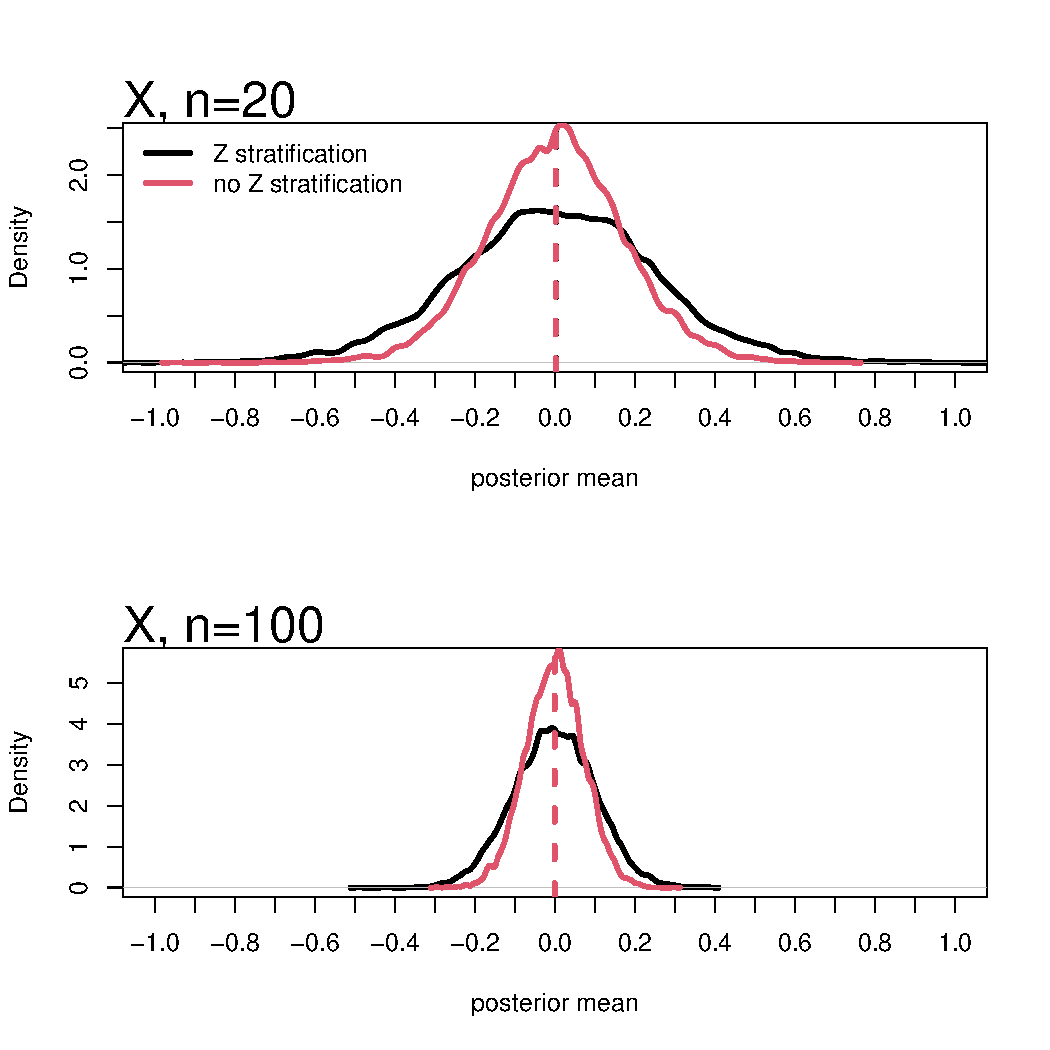
\includegraphics[scale=0.45]{pipefork1_samplesize2.pdf}}]
	{Careful what you control for (though)}
	
	under the \textcolor{blue}{NO stratification model}, \\
	the larger the sample size,
	%
	\begin{itemize}
		%
		\item the more \textcolor{blue}{certain} you are about your \alert{correct} estimates
		%
		\item $Z$ now works as a \textcolor{blue}{precision parasite} \\
		{\small i.e. conditioning on $Z$ reduces variation on $X$, leaving less variability that can explain outcome $Y$}
		%
	\end{itemize}
	%
\end{lhframe}
%
%
\begin{frame}
	{Not all is bad (though)}
	%
	\begin{columns}
		%
		\begin{column}{0.5\textwidth}
			%
			\begin{figure}
				\includegraphics[scale=0.8]{pipefork1_code3.png}
				\caption*{(c) R code}
			\end{figure}
			%
			\textcolor{blue}{Implications},
			%
			\begin{itemize}
				\item \ndsep{X}{Y} \\
				\item \dsep{X}{Y} \\
				\item \dsep{Z}{Y} \\
			\end{itemize}
			%
		\end{column}
		%
		\begin{column}{0.5\textwidth}  
			%
			\begin{equ}
				%
				M = \left\{ \begin{aligned} 
					Z \leftarrow & \; f_{Z}(U_{Z}) \\
					X \leftarrow & \; f_{X}(U_{X}) \\
					M \leftarrow & \; f_{M}(X, Z, U_{M}) \\
					Y \leftarrow & \; f_{Y}(M, U_{Y}) \\
					U \sim & \; P(\pmb{U})
				\end{aligned} \right
				%
				\caption*{(a) structural model}
				%
			\end{equ}
			%
			\begin{figure}
				%
				\begin{tikzpicture}
					% nodes
					\node[formula] at (-2,0.8) {$U_{Z}$};
					\node[formula] at (-1,1) {$Z$};
					\node[formula] at (-2,0) {$U_{X}$};
					\node[formula] at (-1,-0.3) {$X$};
					\node[formula] at (1,1) {$U_{M}$};
					\node[formula] at (0,-0.3) {$M$};
					\node[formula] at (1,-0.3) {$Y$};
					\node[formula] at (2,0) {$U_{Y}$};
					
					% paths
					\draw [{Circle [open]}-{latex}](-1.7,0.75)--(-1,0.75); % Uz->Z
					%\draw [{Circle[color=red]}-{latex}](-0.95,0.8)--(-0.95,0.05); % Z->X
					\draw [{Circle[color=red]}-{latex}](-1,0.75)--(-0.05,0.05); % Z->M
					\draw [{Circle [open]}-{latex}](-1.7,0)--(-1,0); % Ux->X
					\draw [{Circle}-{latex}](-1,0)--(-0.05,0); % X->M
					\draw [{Circle[open]}-{latex}](1,0.8)--(0,0.05); % Um->M
					\draw [{Circle}-{latex}](-0.05,0)--(0.9,0); % M->Y
					\draw [{Circle [open]}-{latex}{Circle}](1.7,0)--(0.9,0); % Uy->Y
				\end{tikzpicture}
				%
				\caption*{(b) causal diagram}
				%
			\end{figure}
			%
		\end{column}
		%
	\end{columns}
	%
\end{frame}
%
%
\begin{lhframe}[rhgraphic={\includegraphics[scale=0.45]{pipefork1_samplesize3.pdf}}]
	{Not all is bad (though)}
	
	under the \textcolor{blue}{stratification model}, \\
	the larger the sample size,
	%
	\begin{itemize}
		%
		\item the more \textcolor{blue}{certain} you are about your \alert{correct} estimates
		%
		\item $Z$ now works as a \textcolor{blue}{precision booster} \\
		{\small i.e. conditioning on $Z$ reduces variation on $Y$ (as $Z$ is a cause of $M$, and $M$ of $Y$), leaving less variability to be explained by $X$}
		%
	\end{itemize}
	%
\end{lhframe}
%
%
%%%%%%%%%%%%%%%%%%%%%%%%%%%%%%%%%%%%%%%%%%%%%%%%%%%%%%%%%%%
\subsection{Pipe/Fork bias: bias amplification}
%%%%%%%%%%%%%%%%%%%%%%%%%%%%%%%%%%%%%%%%%%%%%%%%%%%%%%%%%%%
%
%
\begin{frame}[t, negative]
	\subsectionpage
\end{frame}
%
%
\begin{frame}
	{Bias amplification\footnote{\citet{McElreath_2020}, chapter 14 (p. 455), \citet{Cinelli_et_al_2021} (p. 5)}}
	%
	\begin{columns}
		%
		\begin{column}{0.5\textwidth}
			%
			also known as,
			%
			\begin{itemize}
				%
				\item (unobserved) omitted variable bias
				\item related to \textcolor{blue}{instrumental variables}
				\item an instance of \textcolor{blue}{fork bias}
				%
			\end{itemize}
			
			research question, 
			%
			\begin{itemize}
				%
				\item \textcolor{blue}{Do $E$ has a (direct) effect on $W$?}
				%
			\end{itemize}
			
			variables,
			%
			\begin{itemize}
				%
				\item Q, instrumental variable \\
				(e.g. quarter of the year)
				\item E, educational level
				\item $U_{X}$, unobservables (e.g. ability)
				\item W, future wages
				%
			\end{itemize}
			%
		\end{column}
		%
		\begin{column}{0.5\textwidth}  
			%
			\begin{equ}
				%
				M = \left\{ \begin{aligned} 
					Q \leftarrow & \; f_{Q}(U_{Q}) \\
					E \leftarrow & \; f_{E}(Q, U_{X}, U_{E}) \\
					W \leftarrow & \; f_{W}(E, U_{X}, U_{W}) \\
					U \sim & \; P(\pmb{U})
				\end{aligned} \right
				%
				\caption*{(a) structural model}
				%
			\end{equ}
			%
			\begin{figure}
				%
				\begin{tikzpicture}
					% nodes
					\node[formula] at (-2,0.8) {$U_{Q}$};
					\node[formula] at (-1,1) {$Q$};
					\node[formula] at (-2,0) {$U_{E}$};
					\node[formula] at (-1,-0.3) {$E$};
					\node[formula] at (0,1) {$U_{X}$};
					\node[formula] at (1,-0.3) {$W$};
					\node[formula] at (2,0) {$U_{W}$};
					
					% paths
					\draw [{Circle [open]}-{latex}](-1.7,0.75)--(-1,0.75); % Uq->Q
					\draw [{Circle[color=red]}-{latex}](-0.95,0.8)--(-0.95,0.05); % Q->E
					\draw [{Circle [open]}-{latex}{Circle}](-1.7,0)--(-0.9,0); % Ue->E
					\draw [-{latex}](-0.9,0)--(0.9,0); % E->W
					\draw [{Circle [open]}-{latex}{Circle}](1.7,0)--(0.9,0); % Uw->W
					\draw [-{latex}](0,0.75)--(-0.95,0.05); % Ux->E
					\draw [{Circle [open]}-{latex}](0,0.8)--(0.9,0.1); % Ux->W
					
					% extra
					\node at (0,-0.25) {$(?)$}; % symbol
				\end{tikzpicture}
				%
				\caption*{(b) causal diagram}
				%
			\end{figure}
			%
		\end{column}
		%
	\end{columns}
	%
\end{frame}
%
%
\begin{frame}
	{Simulation setting}
	%
	\begin{columns}
		%
		\begin{column}{0.5\textwidth}
			%
			\begin{figure}
				\includegraphics[scale=0.8]{pipefork2_code.png}
				\caption*{(c) R code}
			\end{figure}
			%
			\textcolor{blue}{Implications},
			%
			\begin{itemize}
				\item \ndsep{E}{W} \\
				%
				\item \dsep{E}{W} \; | $U_{X}$ {\small (impossible) }
				%
				\item \dsep{Q}{$U_{X}$} \\ {\small (cannot be tested) } \\
				%
				\item \ndsep{Q}{E} \\
				%
				\item \dsep{Q}{W} \; | E {\small (cannot be tested) } \\
				{\small \textcolor{blue}{(exclusion restriction)} }\\
			\end{itemize}
			%
		\end{column}
		%
		\begin{column}{0.5\textwidth}  
			%
			\begin{equ}
				%
				M = \left\{ \begin{aligned} 
					Q \leftarrow & \; f_{Q}(U_{Q}) \\
					E \leftarrow & \; f_{E}(Q, U_{X}, U_{E}) \\
					W \leftarrow & \; f_{W}(U_{X}, U_{W}) \\
					U \sim & \; P(\pmb{U})
				\end{aligned} \right
				%
				\caption*{(a) structural model}
				%
			\end{equ}
			%
			\begin{figure}
				%
				\begin{tikzpicture}
					% nodes
					\node[formula] at (-2,0.8) {$U_{Q}$};
					\node[formula] at (-1,1) {$Q$};
					\node[formula] at (-2,0) {$U_{E}$};
					\node[formula] at (-1,-0.3) {$E$};
					\node[formula] at (0,1) {$U_{X}$};
					\node[formula] at (1,-0.3) {$W$};
					\node[formula] at (2,0) {$U_{W}$};
					
					% paths
					\draw [{Circle [open]}-{latex}](-1.7,0.75)--(-1,0.75); % Uq->Q
					\draw [{Circle [color=red]}-{latex}](-0.95,0.8)--(-0.95,0.05); % Q->E
					\draw [{Circle [open]}-{latex}{Circle}](-1.7,0)--(-0.9,0); % Ue->E
					%\draw [-{latex}](-0.9,0)--(0.9,0); % E->W
					\draw [{Circle [open]}-{latex}{Circle}](1.7,0)--(0.9,0); % Uw->W
					\draw [-{latex}](0,0.75)--(-0.95,0.05); % Ux->E
					\draw [{Circle [open]}-{latex}](0,0.8)--(0.9,0.1); % Ux->W
				\end{tikzpicture}
				%
				\caption*{(b) causal diagram}
				%
			\end{figure}
			%
		\end{column}
		%
	\end{columns}
	%
\end{frame}
%
%
\begin{lhframe}[rhgraphic={\includegraphics[scale=0.4]{pipefork2_panel.pdf}}]
	{``Eyeballing" analysis}
	
	based on \textcolor{blue}{correlation analysis},
	%
	\begin{itemize}
		%
		\item $cor(Q, E)>0$ and $cor(E, W)>0$ goes in line of our ``rudimentary" understanding of the data.
		%
		\item $cor(Q, W)>0$ tells you about the \textcolor{blue}{exclusion restriction}? \\
		{\small (hint: No)}
		%
		\item we \textcolor{blue}{might NOT include} $Q$ as a covariate in our statistical model \\
		{\small (but is the instrumental variable!!!)}
		%
	\end{itemize}
	%
\end{lhframe}
%
%
\begin{lhframe}[rhgraphic={\includegraphics[scale=0.3]{pipefork2_reg.png}}]
	{Regression, regression!!}
	
	based on \textcolor{blue}{statistical analysis},
	%
	\begin{itemize}
		%
		\item two different stories \\
		{\small (which model is the ``truth"?) }
		\item one is ``worse"/``better" than the other?
		\item are both wrong?
		%
	\end{itemize}
	%
\end{lhframe}
%
%
\begin{lhframe}[rhgraphic={\includegraphics[scale=0.45]{pipefork2_samplesize.pdf}}]
	{I'll get more data!!}
	
	imagine we can continue sampling,
	%
	\begin{itemize}
		%
		\item top: $10,000$ samples $n=20$
		\item bottom: $10,000$ samples $n=100$
		%
	\end{itemize}
	
	under the \textcolor{blue}{incorrect model}, \\
	the larger the sample size,
	%
	\begin{itemize}
		%
		\item the more \textcolor{blue}{certain} you are about your \textcolor{blue}{biased} estimates \\
		{\small (under the any model!!)}
		%
	\end{itemize}
	%
\end{lhframe}
%
%
\begin{frame}
	{Yo, what is going on??}
	%
	\begin{columns}
		%
		\begin{column}{0.5\textwidth}
			%
			based on \textcolor{blue}{DAG} and \textcolor{blue}{statistical model},
			%
			\begin{itemize}
				%
				\item the 2nd D-separation rule requires control on any noncollider to block the \textcolor{blue}{backdoor path}, \\
				i.e. \dsep{E}{W} \; | $U_{X}$ \\
				{\small (but $U_{X}$  is unobservable)}
				%
				\item if we use $Q$ in the model, the 3rd D-separation rule kicks in: \\
				\textcolor{blue}{``A collider that has been conditioned on does not block a path."}\\
				i.e. \ndsep{Q}{$U_{X}$} \; | E \\
				{(e.g. switch, electricity, and light bulb)}
				%
			\end{itemize}
			%
		\end{column}
		%
		\begin{column}{0.5\textwidth}  
			%
			\begin{equ}
				%
				M = \left\{ \begin{aligned} 
					Q \leftarrow & \; f_{Q}(U_{Q}) \\
					E \leftarrow & \; f_{E}(Q, U_{X}, U_{E}) \\
					W \leftarrow & \; f_{W}(E, U_{X}, U_{W}) \\
					U \sim & \; P(\pmb{U})
				\end{aligned} \right
				%
				\caption*{(a) structural model}
				%
			\end{equ}
			%
			\begin{figure}
				%
				\begin{tikzpicture}
					% nodes
					\node[formula] at (-2,0.8) {$U_{Q}$};
					\node[formula] at (-1,1) {$Q$};
					\node[formula] at (-2,0) {$U_{E}$};
					\node[formula] at (-1,-0.3) {$E$};
					\node[formula] at (0,1) {$U_{X}$};
					\node[formula] at (1,-0.3) {$W$};
					\node[formula] at (2,0) {$U_{W}$};
					
					% paths
					\draw [{Circle [open]}-{latex}](-1.7,0.75)--(-1,0.75); % Uq->Q
					\draw [{Circle[color=red]}-{latex}](-0.95,0.8)--(-0.95,0.05); % Q->E
					\draw [{Circle [open]}-{latex}{Circle}](-1.7,0)--(-0.9,0); % Ue->E
					\draw [-{latex}](-0.9,0)--(0.9,0); % E->W
					\draw [{Circle [open]}-{latex}{Circle}](1.7,0)--(0.9,0); % Uw->W
					\draw [-{latex}](0,0.75)--(-0.95,0.05); % Ux->E
					\draw [{Circle [open]}-{latex}](0,0.8)--(0.9,0.1); % Ux->W
					
					% extra
					\node at (0,-0.25) {$(?)$}; % symbol
				\end{tikzpicture}
				%
				\caption*{(b) causal diagram}
				%
			\end{figure}
			%
		\end{column}
		%
	\end{columns}
	%
\end{frame}
%
%
\begin{frame}
	{Yo, what is going on??}
	%
	\begin{columns}
		%
		\begin{column}{0.5\textwidth}
			%
			open paths?:
			%
			\begin{itemize}
				\item $E \rightarrow W$
				\item $E \rightarrow U_{x} \rightarrow W$
				\item $E \rightarrow U_{x} \rightarrow Q \rightarrow E \rightarrow W$
				\item $E \rightarrow U_{x} \rightarrow Q \rightarrow E \rightarrow U_{X} \rightarrow  W$
			\end{itemize} 
			%
		\end{column}
		%
		\begin{column}{0.5\textwidth}  
			%
			\begin{equ}
				%
				M = \left\{ \begin{aligned} 
					Q \leftarrow & \; f_{Q}(U_{Q}) \\
					E \leftarrow & \; f_{E}(Q, U_{X}, U_{E}) \\
					W \leftarrow & \; f_{W}(E, U_{X}, U_{W}) \\
					U \sim & \; P(\pmb{U})
				\end{aligned} \right
				%
				\caption*{(a) structural model}
				%
			\end{equ}
			%
			\begin{figure}
				%
				\begin{tikzpicture}
					% nodes
					\node[formula] at (-2,0.8) {$U_{Q}$};
					\node[formula] at (-1,1) {$Q$};
					\node[formula] at (-2,0) {$U_{E}$};
					\node[formula] at (-1,-0.3) {$E$};
					\node[formula] at (0,1) {$U_{X}$};
					\node[formula] at (1,-0.3) {$W$};
					\node[formula] at (2,0) {$U_{W}$};
					
					% paths
					\draw [{Circle [open]}-{latex}](-1.7,0.75)--(-1,0.75); % Uq->Q
					\draw [{Circle[color=red]}-{latex}](-0.95,0.8)--(-0.95,0.05); % Q->E
					\draw [{Circle [open]}-{latex}{Circle}](-1.7,0)--(-0.9,0); % Ue->E
					\draw [-{latex}](-0.9,0)--(0.9,0); % E->W
					\draw [{Circle [open]}-{latex}{Circle}](1.7,0)--(0.9,0); % Uw->W
					\draw [-{latex}](0,0.75)--(-0.95,0.05); % Ux->E
					\draw [{Circle [open]}-{latex}](0,0.8)--(0.9,0.1); % Ux->W
					
					% extra
					\node at (0,-0.25) {$(?)$}; % symbol
				\end{tikzpicture}
				%
				\caption*{(b) causal diagram}
				%
			\end{figure}
			%
		\end{column}
		%
	\end{columns}
	%
\end{frame}
%
%
\begin{frame}
	{What should I do then??}
	%
	\begin{columns}
		%
		\begin{column}{0.5\textwidth}
			%
			\begin{equ}
				%
				\begin{aligned} 
					{W \choose E} \sim & \; MVN \left[ {\mu_{W} \choose \mu_{E}}, \pmb{\Sigma} \right] \\
					\mu_{W} = & \; \alpha_{W} + \beta_{EW} E \\
					\mu_{E} = & \; \alpha_{E} + \beta_{QE} Q
				\end{aligned}
				%
				\caption*{(c) probabilistic model}
				%
			\end{equ}
			%
			based on \textcolor{blue}{DAG} and \textcolor{blue}{statistical model}, \\
			use the knowledge of the system
			%
			\begin{itemize}
				%
				\item one model for $Q \rightarrow E$
				%
				\item one model for $E \rightarrow W$
				%
				\item use the knowledge that $cov(E,W)>0$ due to unobserved confounder $U_{X}$, \\
				(i.e. $cov(E,W) = \pmb{\Sigma} = \pmb{S} \pmb{R} \pmb{S}$)
				%
			\end{itemize}
			%
		\end{column}
		%
		\begin{column}{0.5\textwidth}  
			%
			\begin{equ}
				%
				M = \left\{ \begin{aligned} 
					Q \leftarrow & \; f_{Q}(U_{Q}) \\
					E \leftarrow & \; f_{E}(Q, U_{X}, U_{E}) \\
					W \leftarrow & \; f_{W}(E, U_{X}, U_{W}) \\
					U \sim & \; P(\pmb{U})
				\end{aligned} \right
				%
				\caption*{(a) structural model}
				%
			\end{equ}
			%
			\begin{figure}
				%
				\begin{tikzpicture}
					% nodes
					\node[formula] at (-2,0.8) {$U_{Q}$};
					\node[formula] at (-1,1) {$Q$};
					\node[formula] at (-2,0) {$U_{E}$};
					\node[formula] at (-1,-0.3) {$E$};
					\node[formula] at (0,1) {$U_{X}$};
					\node[formula] at (1,-0.3) {$W$};
					\node[formula] at (2,0) {$U_{W}$};
					
					% paths
					\draw [{Circle [open]}-{latex}](-1.7,0.75)--(-1,0.75); % Uq->Q
					\draw [{Circle[color=red]}-{latex}](-0.95,0.8)--(-0.95,0.05); % Q->E
					\draw [{Circle [open]}-{latex}{Circle}](-1.7,0)--(-0.9,0); % Ue->E
					\draw [-{latex}](-0.9,0)--(0.9,0); % E->W
					\draw [{Circle [open]}-{latex}{Circle}](1.7,0)--(0.9,0); % Uw->W
					\draw [-{latex}](0,0.75)--(-0.95,0.05); % Ux->E
					\draw [{Circle [open]}-{latex}](0,0.8)--(0.9,0.1); % Ux->W
					
					% extra
					\node at (0,-0.25) {$(?)$}; % symbol
				\end{tikzpicture}
				%
				\caption*{(b) causal diagram}
				%
			\end{figure}
			%
		\end{column}
		%
	\end{columns}
	%
\end{frame}
%
%
\begin{lhframe}[rhgraphic={\includegraphics[scale=0.7]{pipefork2_reg3.png}}]
	{did it worked???}
	
	based on \textcolor{blue}{DAG} and \textcolor{blue}{bayesian} statistical analysis,
	%
	\begin{itemize}
		%
		\item appropriate value estimated, \\
		{\small \textcolor{blue}{(assuming our DAG is true)} }
		%
		\item it picks up some of the unobserved correlation $R[1,2]$
		%
	\end{itemize}
	%
\end{lhframe}
%
%
\begin{lhframe}[rhgraphic={\includegraphics[scale=0.30]{pipefork2_reg4.png}}]
	{did it worked???}
	
	frequentists guys apply \\
	\textcolor{blue}{Two Stage Least Squares (2SLS)}\footnote{\citet{Hanck_et_al_2021}, section $12.1$, \\
		See \citet{McElreath_2020} chapter 14 (p. 460) for a discussion on the method.}:
	\begin{itemize}
		%
		\item regress $E \leftarrow Q$, 
		%
		\item predict $\hat{E}$,
		%
		\item regress $W \leftarrow \hat{E}$
		%
	\end{itemize}
	%
	\begin{figure}
		\includegraphics[scale=0.7]{pipefork2_code2.png}
	\end{figure}
	%
\end{lhframe}
%
%
\begin{frame}
	{Similar case, contextual confounds\footnote{\citet{McElreath_2022}, lecture 6}}
	%
	\begin{columns}
		%
		\begin{column}{0.5\textwidth}
			%
			research question, 
			%
			\begin{itemize}
				%
				\item \textcolor{blue}{Does $W$ has an effect on $L$?}
				\item should we include $H$ in our model?
				%
			\end{itemize}
			
			variables,
			%
			\begin{itemize}
				%
				\item W, win the lottery 
				\item H, happiness
				\item $U_{X}$, contextual confound 
				\item L, lifespan
				%
			\end{itemize}
			
			Short answer;
			%
			\begin{itemize}
				%
				\item for \textcolor{blue}{total effects}: No \\
				{\small (two question marks together)}
				\item for \textcolor{blue}{direct effect} of $H \rightarrow L$: \\
				will be always counfounded
				%
			\end{itemize}
		\end{column}
		%
		\begin{column}{0.5\textwidth}  
			%
			\begin{equ}
				%
				M = \left\{ \begin{aligned} 
					W \leftarrow & \; f_{W}(U_{W}) \\
					H \leftarrow & \; f_{H}(W, U_{X}, U_{H}) \\
					L \leftarrow & \; f_{L}(H, U_{X}, U_{L}) \\
					U \sim & \; P(\pmb{U})
				\end{aligned} \right
				%
				\caption*{(a) structural model}
				%
			\end{equ}
			%
			\begin{figure}
				%
				\begin{tikzpicture}
					% nodes
					\node[formula] at (-2,0.8) {$U_{W}$};
					\node[formula] at (-1,1) {$W$};
					\node[formula] at (-2,0) {$U_{H}$};
					\node[formula] at (-1,-0.3) {$H$};
					\node[formula] at (0,1) {$U_{X}$};
					\node[formula] at (1,-0.3) {$L$};
					\node[formula] at (2,0) {$U_{L}$};
					
					% paths
					\draw [{Circle [open]}-{latex}](-1.7,0.75)--(-1,0.75); % Uw->W
					\draw [{Circle}-{latex}](-0.95,0.8)--(-0.95,0.05); % W->H
					\draw [{Circle [open]}-{latex}](-1.7,0)--(-1,0); % Uh->H
					\draw [{Circle[color=red]}-{latex}](-1.03,0)--(0.9,0); % H->L
					\draw [{Circle [open]}-{latex}{Circle}](1.7,0)--(0.9,0); % Ul->L
					\draw [-{latex}](0,0.75)--(-0.95,0.05); % Ux->H
					\draw [{Circle [open]}-{latex}](0,0.8)--(0.9,0.1); % Ux->L
					
					% extra
					\node at (0,-0.25) {$(?)$}; % symbol
					\node at (-1.25,0.35) {$(?)$}; % symbol
				\end{tikzpicture}
				%
				\caption*{(b) causal diagram}
				%
			\end{figure}
			%
		\end{column}
		%
	\end{columns}
	%
\end{frame}
%
%
%%%%%%%%%%%%%%%%%%%%%%%%%%%%%%%%%%%%%%%%%%%%%%%%%%%%%%%%%%%
\subsection{Collider bias: M-bias}
%%%%%%%%%%%%%%%%%%%%%%%%%%%%%%%%%%%%%%%%%%%%%%%%%%%%%%%%%%%
%
%
\begin{frame}[t, negative]
	\subsectionpage
\end{frame}
%
%
\begin{frame}
	{M-bias\footnote{\citet{McElreath_2022}, lecture 6; \citet{Cinelli_et_al_2021} (p. 4)}}
	%
	\begin{columns}
		%
		\begin{column}{0.5\textwidth}
			%
			case of,
			%
			\begin{itemize}
				%
				\item bias on pre-treatment variable
				%
			\end{itemize}
			
			research question, 
			%
			\begin{itemize}
				%
				\item \textcolor{blue}{Should we include $Z$ in our model?}
				%
			\end{itemize}
			
			variables,
			%
			\begin{itemize}
				%
				\item $Z$, ``health" quality of friends \\
				{\small (defined as a continuum)}
				\item $X$, health of individual $1$
				\item $U_{1}$, hobbies of individual $1$
				\item $Y$, health of individual $2$
				\item $U_{2}$, hobbies of individual $2$ 
				%
			\end{itemize}
			%
		\end{column}
		%
		\begin{column}{0.5\textwidth}  
			%
			\begin{equ}
				%
				M = \left\{ \begin{aligned} 
					X \leftarrow & \; f_{X}(U_{1},U_{X}) \\
					Z \leftarrow & \; f_{Z}(U_{1},U_{2},U_{Z}) \\
					Y \leftarrow & \; f_{Y}(X, U_{2}, U_{Y}) \\
					U \sim & \; P(\pmb{U})
				\end{aligned} \right
				%
				\caption*{(a) structural model}
				%
			\end{equ}
			%
			\begin{figure}
				%
				\begin{tikzpicture}
					% nodes
					\node[formula] at (-1,1) {$U_{1}$};
					\node[formula] at (-2,0) {$U_{X}$};
					\node[formula] at (-1,-0.3) {$X$};
					\node[formula] at (1,1.7) {$U_{Z}$};
					\node[formula] at (-0.1,1.05) {$Z$};
					\node[formula] at (1,1) {$U_{2}$};
					\node[formula] at (2,0) {$U_{Y}$};
					\node[formula] at (1,-0.3) {$Y$};
					
					% paths
					\draw [{Circle[open]}-{latex}](-0.95,0.8)--(-0.95,0.05); % U1->X
					\draw [-{latex}{Circle}](-0.9,0.75)--(0,0.75); % U1->Z
					\draw [{Circle[open]}-{latex}{Circle}](-1.7,0)--(-0.9,0); % Ux->X
					\draw [-{latex}](-0.9,0)--(0.9,0); % X->Y
					\draw [{Circle [open]}-{latex}{Circle}](1.7,0)--(0.9,0); % Uy->y
					\draw [{Circle [open]}-{latex}](0.9,1.5)--(0,0.8); % Uz->Z
					\draw [-{latex}](0.90,0.75)--(0,0.75); % U2->Z
					\draw [{Circle[open]}-{latex}](0.95,0.8)--(0.95,0.05); % U2->Y
					
					% extra
					\node at (0,-0.25) {$(?)$}; % symbol
				\end{tikzpicture}
				%
				\caption*{(b) causal diagram}
				%
			\end{figure}
			%
		\end{column}
		%
	\end{columns}
	%
\end{frame}
%
%
\begin{frame}
	{Simulation setting}
	%
	\begin{columns}
		%
		\begin{column}{0.5\textwidth}
			%
			\begin{figure}
				\includegraphics[scale=0.8]{collider4_code.png}
				\caption*{(c) R code}
			\end{figure}
			%
			\textcolor{blue}{Implications},
			%
			\begin{itemize}
				\item \dsep{X}{Y} \\
				\item \ndsep{X}{Y} \; | Z 
			\end{itemize}
			%
		\end{column}
		%
		\begin{column}{0.5\textwidth}  
			%
			\begin{equ}
				%
				M = \left\{ \begin{aligned} 
					X \leftarrow & \; f_{X}(U_{1},U_{X}) \\
					Z \leftarrow & \; f_{Z}(U_{1},U_{2},U_{Z}) \\
					Y \leftarrow & \; f_{Y}(X, U_{2}, U_{Y}) \\
					U \sim & \; P(\pmb{U})
				\end{aligned} \right
				%
				\caption*{(a) structural model}
				%
			\end{equ}
			%
			\begin{figure}
				%
				\begin{tikzpicture}
					% nodes
					\node[formula] at (-1,1) {$U_{1}$};
					\node[formula] at (-2,0) {$U_{X}$};
					\node[formula] at (-1,-0.3) {$X$};
					\node[formula] at (1,1.7) {$U_{Z}$};
					\node[formula] at (-0.1,1.05) {$Z$};
					\node[formula] at (1,1) {$U_{2}$};
					\node[formula] at (2,0) {$U_{Y}$};
					\node[formula] at (1,-0.3) {$Y$};
					
					% paths
					\draw [{Circle[open]}-{latex}](-0.95,0.8)--(-0.95,0.05); % U1->X
					\draw [-{latex}{Circle}](-0.9,0.75)--(0,0.75); % U1->Z
					\draw [{Circle[open]}-{latex}{Circle}](-1.7,0)--(-0.9,0); % Ux->X
					%\draw [-{latex}](-0.9,0)--(0.9,0); % X->Y
					\draw [{Circle [open]}-{latex}{Circle}](1.7,0)--(0.9,0); % Uy->y
					\draw [{Circle [open]}-{latex}](0.9,1.5)--(0,0.8); % Uz->Z
					\draw [-{latex}](0.90,0.75)--(0,0.75); % U2->Z
					\draw [{Circle[open]}-{latex}](0.95,0.8)--(0.95,0.05); % U2->Y
				\end{tikzpicture}
				%
				\caption*{(b) causal diagram}
				%
			\end{figure}
			%
		\end{column}
		%
	\end{columns}
	%
\end{frame}
%
%
\begin{lhframe}[rhgraphic={\includegraphics[scale=0.40]{collider4_panel.pdf}}]
	{Descriptive analysis}
	
	based on \textcolor{blue}{descriptive analysis},
	%
	\begin{itemize}
		%
		\item $Cor(X, Y) \approx 0$, quite low
		%
		\item larger $Cor(Z,Y)$, while $Cor(Z,X)$ is not high enough to discard it as a cause of multicollinearity,
		%
		\item we \textcolor{blue}{might include} $Z$ rather than $X$ \\
		{\small (but the effect of $X$ is our interest!!)}
		%
		\item then we include $Z$ and $X$
		%
	\end{itemize}
	%
\end{lhframe}
%
%
\begin{lhframe}[rhgraphic={\includegraphics[scale=0.3]{collider4_reg.png}}]
	{Again regression!!}
	
	based on \textcolor{blue}{statistical analysis},
	%
	\begin{itemize}
		%
		\item $X$ does not have an effect of $Y$, \\
		{\small (in the first nor the second model)}
		%
		\item but $X$ has an (non-negligible) effect when $Z$ is in the model \\
		{\small (but we do not reject the null)}
		%
		\item The increase of the $X$ effect might lead you to think that with more data, we can reject the null \\
		{\small (and you would be right!!)} \\
		%
		\item But is it correct to include $Z$?
		%
	\end{itemize}
	%
\end{lhframe}
%
%
\begin{lhframe}[rhgraphic={\includegraphics[scale=0.45]{collider4_samplesize.pdf}}]
	{Ok, I get it!!, more data, more wrong!!}
	
	imagine we can continue sampling,
	%
	\begin{itemize}
		%
		\item top: $10,000$ samples $n=20$
		\item bottom: $10,000$ samples $n=100$
		%
	\end{itemize}
	
	under the \textcolor{blue}{``incorrect" model}, \\
	the larger the sample size,
	%
	\begin{itemize}
		%
		\item the more \textcolor{blue}{certain} you are about your \textcolor{blue}{biased} estimates \\
		{\small (with enough you could reject the null)}
		%
	\end{itemize}
	%
\end{lhframe}
%
%
\begin{frame}
	{The dream team strikes back!!}
	%
	\begin{columns}
		%
		\begin{column}{0.5\textwidth}
			%
			based on \textcolor{blue}{DAG} and \textcolor{blue}{statistical model},
			%
			\begin{itemize}
				%
				\item the 3rd D-separation states that a collider that has been conditioned on \textcolor{blue}{does not block a path}, \\
				in this case: $X \rightarrow U_{1} \rightarrow Z \rightarrow U_{2} \rightarrow Y$ \\
				i.e. \ndsep{X}{Y} \; | Z \\
				%
				\item therefore if we want to find the direct effect of $X \rightarrow Y$, we \textcolor{blue}{should not} stratify by $Z$
				%
			\end{itemize}
			%
		\end{column}
		%
		\begin{column}{0.5\textwidth}  
			%
			\begin{equ}
				%
				M = \left\{ \begin{aligned} 
					X \leftarrow & \; f_{X}(U_{1},U_{X}) \\
					Z \leftarrow & \; f_{Z}(U_{1},U_{2},U_{Z}) \\
					Y \leftarrow & \; f_{Y}(X, U_{2}, U_{Y}) \\
					U \sim & \; P(\pmb{U})
				\end{aligned} \right
				%
				\caption*{(a) structural model}
				%
			\end{equ}
			%
			\begin{figure}
				%
				\begin{tikzpicture}
					% nodes
					\node[formula] at (-1,1) {$U_{1}$};
					\node[formula] at (-2,0) {$U_{X}$};
					\node[formula] at (-1,-0.3) {$X$};
					\node[formula] at (1,1.7) {$U_{Z}$};
					\node[formula] at (-0.1,1.05) {$Z$};
					\node[formula] at (1,1) {$U_{2}$};
					\node[formula] at (2,0) {$U_{Y}$};
					\node[formula] at (1,-0.3) {$Y$};
					
					% paths
					\draw [{Circle[open]}-{latex}](-0.95,0.8)--(-0.95,0.05); % U1->X
					\draw [-{latex}{Circle}](-0.9,0.75)--(0,0.75); % U1->Z
					\draw [{Circle[open]}-{latex}{Circle}](-1.7,0)--(-0.9,0); % Ux->X
					\draw [-{latex}](-0.9,0)--(0.9,0); % X->Y
					\draw [{Circle [open]}-{latex}{Circle}](1.7,0)--(0.9,0); % Uy->y
					\draw [{Circle [open]}-{latex}](0.9,1.5)--(0,0.8); % Uz->Z
					\draw [-{latex}](0.90,0.75)--(0,0.75); % U2->Z
					\draw [{Circle[open]}-{latex}](0.95,0.8)--(0.95,0.05); % U2->Y
					
					% extra
					\node at (0,-0.25) {$(?)$}; % symbol
				\end{tikzpicture}
				%
				\caption*{(b) causal diagram}
				%
			\end{figure}
			%
		\end{column}
		%
	\end{columns}
	%
\end{frame}
%
%
\begin{lhframe}[rhgraphic={\includegraphics[scale=0.5]{collider4_reg1.png}}]
	{The dream team strikes back!!}
	
	based on \textcolor{blue}{DAG} and \textcolor{blue}{statistical analysis},
	%
	\begin{itemize}
		%
		\item the model that answers our research question is the first one, \\
		{\small \textcolor{blue}{(assuming our DAG is true)} }
		%
	\end{itemize}
	%
\end{lhframe}
%
%
%%%%%%%%%%%%%%%%%%%%%%%%%%%%%%%%%%%%%%%%%%%%%%%%%%%%%%%%%%%
\subsection{Descendant bias: case control}
%%%%%%%%%%%%%%%%%%%%%%%%%%%%%%%%%%%%%%%%%%%%%%%%%%%%%%%%%%%
%
%
\begin{frame}[t, negative]
	\subsectionpage
\end{frame}
%
%
\begin{frame}
	{Case control\footnote{\citet{McElreath_2022}, lecture 06; \citet{Cinelli_et_al_2021} (p. 8)}}
	%
	\begin{columns}
		%
		\begin{column}{0.5\textwidth}
			%
			also, 
			%
			\begin{itemize}
				%
				\item an instance of \textcolor{blue}{descendant bias}
				%
			\end{itemize}
			
			research question, 
			%
			\begin{itemize}
				%
				\item \textcolor{blue}{Does $E$ has a (direct) effect on $H$?}
				\item Should we include $I$ on our model?
				%
			\end{itemize}
			
			variables,
			%
			\begin{itemize}
				%
				\item E, education 
				\item H, hours in occupation \\
				{\small (standardized)}
				\item I, income
				%
			\end{itemize}
			%
		\end{column}
		%
		\begin{column}{0.5\textwidth}  
			%
			\begin{equ}
				%
				M = \left\{ \begin{aligned} 
					E \leftarrow & \; f_{E}(U_{E}) \\
					H \leftarrow & \; f_{H}(E,U_{H}) \\
					I \leftarrow & \; f_{I}(H,U_{I}) \\
					U \sim & \; P(\pmb{U})
				\end{aligned} \right
				%
				\caption*{(a) structural model}
				%
			\end{equ}
			%
			\begin{figure}
				%
				\begin{tikzpicture}
					% nodes
					\node[formula] at (-2,0) {$U_{E}$};
					\node[formula] at (-1,-0.3) {$E$};
					\node[formula] at (1,1.5) {$U_{I}$};
					\node[formula] at (0,1) {$I$};
					\node[formula] at (2,0) {$U_{H}$};
					\node[formula] at (1,-0.3) {$H$};
					
					% paths
					\draw [{Circle [open]}-{latex}{Circle}](-1.7,0)--(-0.9,0); % Ue->E
					\draw [-{latex}](-0.9,0)--(0.9,0); % E->H
					\draw [{Circle [open]}-{latex}{Circle}](1.7,0)--(0.9,0); % Uh->H
					\draw [-{latex}{Circle}](0.95,0.05)--(0,0.8); % H->I
					\draw [{Circle [open]}-{latex}](0.9,1.3)--(0.1,0.8); % Ui->I
					
					% extra
					\node at (0,-0.25) {$(?)$}; % symbol
				\end{tikzpicture}
				%
				\caption*{(b) causal diagram}
				%
			\end{figure}
			%
		\end{column}
		%
	\end{columns}
	%
\end{frame}
%
%
\begin{frame}
	{Simulation setting}
	%
	\begin{columns}
		%
		\begin{column}{0.5\textwidth}
			%
			\begin{figure}
				\includegraphics[scale=0.8]{descendant1_code.png}
				\caption*{(c) R code}
			\end{figure}
			%
			\textcolor{blue}{Implications},
			%
			\begin{itemize}
				\item \ndsep{E}{H} \\
				\item \dsep{E}{I} \; | H
			\end{itemize}
			%
		\end{column}
		%
		\begin{column}{0.5\textwidth}  
			%
			\begin{equ}
				%
				M = \left\{ \begin{aligned} 
					E \leftarrow & \; f_{E}(U_{E}) \\
					H \leftarrow & \; f_{H}(E,U_{H}) \\
					I \leftarrow & \; f_{I}(H,U_{I}) \\
					U \sim & \; P(\pmb{U})
				\end{aligned} \right
				%
				\caption*{(a) structural model}
				%
			\end{equ}
			%
			\begin{figure}
				%
				\begin{tikzpicture}
					% nodes
					\node[formula] at (-2,0) {$U_{E}$};
					\node[formula] at (-1,-0.3) {$E$};
					\node[formula] at (1,1.5) {$U_{I}$};
					\node[formula] at (0,1) {$I$};
					\node[formula] at (2,0) {$U_{H}$};
					\node[formula] at (1,-0.3) {$H$};
					
					% paths
					\draw [{Circle [open]}-{latex}{Circle}](-1.7,0)--(-0.9,0); % Ue->E
					\draw [-{latex}](-0.9,0)--(0.9,0); % E->H
					\draw [{Circle [open]}-{latex}{Circle}](1.7,0)--(0.9,0); % Uh->H
					\draw [-{latex}{Circle}](0.95,0.05)--(0,0.8); % H->I
					\draw [{Circle [open]}-{latex}](0.9,1.3)--(0.1,0.8); % Ui->I
				\end{tikzpicture}
				%
				\caption*{(b) causal diagram}
				%
			\end{figure}
			%
		\end{column}
		%
	\end{columns}
	%
\end{frame}
%
%
\begin{lhframe}[rhgraphic={\includegraphics[scale=0.4]{descendant1_panel.pdf}}]
	{``Eyeballing" analysis}
	
	based on \textcolor{blue}{correlation analysis},
	%
	\begin{itemize}
		%
		\item $cor(E, I)<0$ does NOT goes in line of our ``rudimentary" understanding of the data.
		%
		\item while $cor(H, I)>0$ indicate the more you work the more you gain \\
		{\small (but is it the only way?)}
		%
		\item since $cor(H, I)$ is high we \textcolor{blue}{might include it} as a covariate in our statistical model \\
		{\small (to improve the precision?)}
		%
	\end{itemize}
	%
\end{lhframe}
%
%
\begin{lhframe}[rhgraphic={\includegraphics[scale=0.3]{descendant1_reg.png}}]
	{Regression, regression!!}
	
	based on \textcolor{blue}{statistical analysis},
	%
	\begin{itemize}
		%
		\item we now have two models with two different ``levels" of effects
		\item which one is the ``truth"?
		%
	\end{itemize}
	%
\end{lhframe}
%
%
\begin{lhframe}[rhgraphic={\includegraphics[scale=0.45]{descendant1_samplesize.pdf}}]
	{The data tell-tell story!!}
	
	imagine we can continue sampling,
	%
	\begin{itemize}
		%
		\item top: $10,000$ samples $n=20$
		\item bottom: $10,000$ samples $n=100$
		%
	\end{itemize}
	
	under the \textcolor{blue}{incorrect model},\\
	the larger the sample size,
	%
	\begin{itemize}
		%
		\item the more \textcolor{blue}{certain} you are about your \textcolor{blue}{biased} estimates
		%
	\end{itemize}
	%
\end{lhframe}
%
%
\begin{frame}
	{The dream team!!}
	%
	\begin{columns}
		%
		\begin{column}{0.5\textwidth}
			%
			based on \textcolor{blue}{DAG} and \textcolor{blue}{statistical model},
			%
			\begin{itemize}
				%
				\item stratifying (controlling) on $I$, we are already explaining variability in $H$ \\
				{\small ($I$ is a descendant of $H$)}
				\item the remaining is explained by $E$ \\
				{\small (big chunk is already explained)}
				%
			\end{itemize}
			%
		\end{column}
		%
		\begin{column}{0.5\textwidth}  
			%
			\begin{equ}
				%
				M = \left\{ \begin{aligned} 
					E \leftarrow & \; f_{E}(U_{E}) \\
					H \leftarrow & \; f_{H}(E,U_{H}) \\
					I \leftarrow & \; f_{I}(H,U_{I}) \\
					U \sim & \; P(\pmb{U})
				\end{aligned} \right
				%
				\caption*{(a) structural model}
				%
			\end{equ}
			%
			\begin{figure}
				%
				\begin{tikzpicture}
					% nodes
					\node[formula] at (-2,0) {$U_{E}$};
					\node[formula] at (-1,-0.3) {$E$};
					\node[formula] at (1,1.5) {$U_{I}$};
					\node[formula] at (0,1) {$I$};
					\node[formula] at (2,0) {$U_{H}$};
					\node[formula] at (1,-0.3) {$H$};
					
					% paths
					\draw [{Circle [open]}-{latex}{Circle}](-1.7,0)--(-0.9,0); % Ue->E
					\draw [-{latex}](-0.9,0)--(0.9,0); % E->H
					\draw [{Circle [open]}-{latex}{Circle}](1.7,0)--(0.9,0); % Uh->H
					\draw [-{latex}{Circle}](0.95,0.05)--(0,0.8); % H->I
					\draw [{Circle [open]}-{latex}](0.9,1.3)--(0.1,0.8); % Ui->I
					
					% extra
					\node at (0,-0.25) {$(?)$}; % symbol
				\end{tikzpicture}
				%
				\caption*{(b) causal diagram}
				%
			\end{figure}
			%
		\end{column}
		%
	\end{columns}
	%
\end{frame}
%
%
\begin{lhframe}[rhgraphic={\includegraphics[scale=0.5]{descendant1_reg1.png}}]
	{the dream team!!}
	
	based on \textcolor{blue}{DAG} and \textcolor{blue}{statistical analysis},
	%
	\begin{itemize}
		%
		\item the less biased model is the first, \\
		{\small \textcolor{blue}{(assuming our DAG is true)} }
		%
	\end{itemize}
	%
\end{lhframe}
%
%
